\documentclass[UTF8,a4paper,12pt]{ctexart}
\usepackage[left=3cm, right=3cm]{geometry}
\usepackage[fontset=mac]{ctex}

\usepackage{amsmath}
\numberwithin{equation}{section}
\renewcommand\thesection{\arabic{section}}
\allowdisplaybreaks[4]       %多行公式中换页
\usepackage{array}
\usepackage[font=small,labelsep=none]{caption}
\usepackage{amssymb}
\usepackage{tikz}
\usepackage{amsthm}
\usepackage{mathrsfs}
\usepackage{float}

\usepackage{dutchcal}
\usepackage{color}
\usepackage{graphicx}    %插入图片 
\usepackage{times}
\usepackage{mathptmx}
\usepackage{fancyhdr} %页眉页脚
\usepackage{booktabs}  %三线表



\pagestyle{fancy}
\fancyhf{}
\fancyfoot[C]{\thepage}

\newcommand*{\circled}[1]{\lower.7ex\hbox{\tikz\draw (0pt, 0pt)%
    circle (.5em) node {\makebox[1em][c]{\small #1}};}}
    
\usepackage{hyperref}  %目录
\hypersetup{colorlinks=true,linkcolor=black}

\renewcommand {\thefigure} {\thesection{}.\arabic{figure}}%设定图片的编号。这样设置的实现效果为图1.1
\renewcommand {\thetable} {\thesection{}.\arabic{table}}


\usepackage{caption}
\captionsetup{font={small},labelsep=quad}%文字5号,之间空一个汉字符位。

\usepackage{appendix}
\usepackage{tocloft} 
\usepackage{titletoc}

\usepackage{setspace}
\usepackage{titlesec}
\setstretch{1.25}


% 设置section字体为黑体三号
\titleformat{\section}{\heiti\zihao{3}\centering}{\thesection}{0.5em}{}[]
% 设置subsection字体为黑体小三号
\titleformat{\subsection}{\heiti\zihao{-3}}{\thesubsection}{0.5em}{}[]
% 设置subsubsection字体为黑体四号
\titleformat{\subsubsection}{\heiti\zihao{4}}{\thesubsubsection}{0.5em}{}[]
%\titlespacing{\section}{0pt}{\baselineskip}{\baselineskip}
%\titlespacing{\section}{0pt}{0pt}{\baselineskip}

% 目录中section的格式
\titlecontents{section}[0pt]{\addvspace{0pt}\filright\heiti\zihao{4}}%
               {\contentspush{\thecontentslabel \quad}}%
               {}{\titlerule*[8pt]{.}\contentspage}
% 目录中subsection的格式
\titlecontents{subsection}[1em]{\addvspace{0pt}\filright\heiti\zihao{5}}%
               {\contentspush{\thecontentslabel \quad}}%
               {}{\titlerule*[8pt]{.}\contentspage}
% 目录中subsubsection的格式
\titlecontents{subsubsection}[2em]{\addvspace{0pt}\filright\songti\zihao{5}}%
               {\contentspush{\thecontentslabel \quad}}%
               {}{\titlerule*[8pt]{.}\contentspage}

\renewcommand{\cftsecleader}{\cftdotfill{\cftdotsep}} %为目录中section补上引导点
               
\makeatletter % 单线页眉
\def\headrule{{\if@fancyplain\let\headrulewidth\plainheadrulewidth\fi%
\hrule\@height 0.5pt \@width\headwidth\vskip1.5pt% 上面线为0.5pt粗
\vskip-2\headrulewidth\vskip-1pt}}     % 与下面正文之间的垂直间距
\makeatother



\setlength{\headheight}{14.48167pt} 
\setlength{\voffset}{-1.14cm}
\setlength{\topmargin}{0cm}
\setlength{\headsep}{2.5cm}


\begin{document}

\thispagestyle{empty}




\begin{center}
\heiti  \zihao{-2} 重庆大学本科学生毕业论文(设计)
\end{center}
%该页为中文扉页。无需页眉页脚,纸质论文应装订在右侧
~\\
\begin{center}
\heiti  \zihao{2} 面向多编程语言的代码检索系统设计与实现
\end{center}
%中文论文标题,1行或2行,黑体,二号,居中。论文题目不得超过36个汉字

~\\
\renewcommand{\headrulewidth}{1pt}
\begin{figure}[htb] 
  \centering
    \center{\includegraphics[width=5cm]  {fig1.png}} 
     \end{figure}
     
~\\
\begin{center}
\heiti\zihao{4}
\begin{tabular}{l}
学\qquad 生:夏劲\\
学\qquad 号:20214966\\
指导教师:刘超\\
专\qquad 业:软件工程\\
\end{tabular}
\end{center}

%此模版适用于理工农医等专业;人文社科类专业按《重庆大学普通本科毕业论文(设计)撰写规范化要求》。  若没有助理指导教师,请删除“助理指导教师姓名”栏。若为校外完成毕业论文(设计),请改为“校外指导教师姓名”即可。  学院、专业填全称。

~\\
\begin{center}
\heiti \zihao{-2} {重庆大学大数据与软件学院}\\
\end{center}

\begin{center}
\heiti \zihao{3} {2025年6月}
\end{center}



\newpage
\thispagestyle{empty}
\setmainfont{Times New Roman}
\begin{center}
\zihao{3}
\textbf{
Undergraduate Thesis (Design) of Chongqing University}
\end{center}
~\\
\begin{center}
\zihao{2}
\textbf{Code Search System for Multi-Programming Languages}
\end{center}

~\\
\renewcommand{\headrulewidth}{1pt}
\begin{figure}[htb] 
  \centering
    \center{\includegraphics[width=5cm]  {fig1.png}} 
     \end{figure}
     

\setmainfont{Times New Roman}
\begin{center}
\zihao{3} 
\textbf{By}  \\
\textbf{Jin Xia}
\end{center}

\begin{center}
\zihao{3} 
\textbf{Supervised by}\\
\textbf{Chao Liu}\\
\end{center}

\begin{center}
\zihao{-2} 
\textbf{Software Engineering}\\ %专业
\textbf{	School of Big Data and Software Engineering}\\ %学院
\textbf{Chongqing University}
\end{center}

\begin{center}
\zihao{3} 
\textbf{June, 2025}
\end{center}


\newpage
\pagestyle{fancy}
\pagenumbering{Roman}

% 设置左侧页眉
\fancyhead[LH]{ \songti\zihao{-5} 重庆大学本科学生毕业论文(设计)}
\fancyhead[RH]{\songti\zihao{-5} 摘要}



\addcontentsline{toc}{section}{摘要}

\section*{摘\quad 要}
随着编程语言的多样化和开源项目的迅速增长,开发者在寻找特定代码片段时面临着越来越大的挑战。现有的代码托管平台主要依赖关键词匹配和特定搜索条件进行检索,效率较低且使用门槛较高。近年来,使用大语言模型赋能各项传统软件成为了工业界和学术界的大趋势。但是大语言模型的部署成本较高,针对特定的任务非常依赖特定的微调训练以及提示词工程,对普通开发者并不友好。为此,本文提出了一种基于大语言模型的代码检索任务工作流。该工作流依赖大模型的自然语言理解能力,将用户的初始搜索词改写为具有特定上下文的查询词,赋予查询词更加准确的查询范围,结合具有跨平台搜索能力检索系统, 最终实现面向多编程语言的代码检索系统。其中核心的工作内容如下:\par
(1)基于大语言模型的查询上下文增强的提示词工程:通过控制变量的试验方法,在同样提示词下对比不同模型的查询改写效果,在同样模型下对比不同提示词的查询改写效果,探索适合用于用户查询上下文的大语言模型和提示词工程。\par
(2)基于分布式系统的跨文件检索平台:设计并实现一个支持多编程语言、多代码仓库的分布式检索系统。该平台能够高效地对大规模代码库进行索引和分片,支持横向扩展,提升检索的并发能力和响应速度。通过引入高效的倒排索引、分布式缓存和负载均衡机制,保障在多用户高并发场景下的稳定性和可用性。\par
(3)基于微服务架构的高可用后台管理平台:构建模块化、可扩展的后台服务体系,将查询改写、检索调度、权限管理等核心功能解耦为独立微服务。每个服务可独立部署和扩展,提升系统的可维护性和容错能力。通过容器化部署和自动化运维工具,实现服务的自动扩缩容和故障自愈,确保平台在大规模访问下的高可用性和稳定性。\par
(4)基于响应式组件的人机友好的前端界面:开发直观易用的前端界面,采用响应式设计以适配不同终端设备。前端集成智能查询、代码高亮、结果聚合与筛选等功能,提升用户的检索体验。通过与后端API的高效交互,实现实时查询反馈和结果的动态展示。\par
本系统在设计过程中高度重视用户体验,前端界面采用现代化响应式设计,整体风格简洁美观,交互流程清晰,极大降低了用户的学习和操作门槛。通过模块化的组件设计,用户可以便捷地进行多条件筛选、结果预览等操作,显著提升了检索的易用性和友好性。在系统实现层面,后端服务采用gRPC协议实现高效的服务间通信,结合Docker容器化部署,确保了系统的高可用性、易扩展性和跨平台兼容性。通过上述设计与实现,系统不仅满足了多编程语言、多平台环境下的高效代码检索需求,也为开发者提供了美观、易用且高性能的检索工具。
~\\
\hspace*{2em}{\heiti \zihao{-4}关键词}:代码搜索;Elasticsearch;gRPC框架;微服务;大模型提示工程\\
%关键字:宋体12磅,行距20磅,段前段后0磅,关键字之间用分号隔开,关键词三个字加粗。

\newpage
\fancyhead[LH]{ \songti\zihao{-5} 重庆大学本科学生毕业论文(设计)}
\fancyhead[RH]{\zihao{-5} ABSTRACT}

\addcontentsline{toc}{section}{ABSTRACT}
\titleformat{\section}[block]{\centering\bfseries\fontspec{Times New Roman}\fontsize{16pt}{20pt}\selectfont}{\thesection}{1em}{}[]

\section*{ABSTRACT}
%ABSTRCT:Times New Roman 加粗三号,段前段后空一行
With the diversification of programming languages and the rapid growth of open-source projects, developers are facing increasing challenges when searching for specific code snippets. Existing code hosting platforms mainly rely on keyword matching and specific search conditions for retrieval, which are often inefficient and have a high barrier to use. In recent years, empowering traditional software with large language models has become a major trend in both industry and academia. However, deploying large language models is costly, and their effectiveness for specific tasks heavily depends on specialized fine-tuning and prompt engineering, making them less accessible to ordinary developers.\par

To address these issues, this thesis proposes a code retrieval workflow based on large language models. This workflow leverages the natural language understanding capabilities of large models to rewrite users’ initial search queries into context-aware queries, thereby providing more accurate search scopes. Combined with a retrieval system capable of cross-platform search, this approach ultimately enables a code retrieval system for multiple programming languages. The core contributions of this work are as follows:\par

(1) Prompt engineering for query context enhancement based on large language models: By conducting controlled experiments, we compare the query rewriting effects of different models under the same prompts, and the effects of different prompts under the same model, to explore suitable large language models and prompt engineering strategies for user query context enhancement.\par

(2) Distributed cross-file retrieval platform: We design and implement a distributed retrieval system that supports multiple programming languages and code repositories. This platform efficiently indexes and shards large-scale codebases, supports horizontal scaling, and improves concurrent retrieval capability and response speed. By introducing efficient inverted indexing, distributed caching, and load balancing mechanisms, the system ensures stability and availability under high-concurrency, multi-user scenarios.\par

(3) Highly available backend management platform based on microservices architecture: We build a modular and extensible backend service system, decoupling core functions such as query rewriting, retrieval scheduling, and access control into independent microservices. Each service can be deployed and scaled independently, improving system maintainability and fault tolerance. Through containerized deployment and automated operation tools, the system achieves automatic scaling and self-healing, ensuring high availability and stability under large-scale access.\par

(4) User-friendly frontend interface based on responsive components: We develop an intuitive and easy-to-use frontend interface with responsive design to adapt to different terminal devices. The frontend integrates intelligent query, code highlighting, result aggregation, and filtering functions to enhance the user retrieval experience. Efficient interaction with backend APIs enables real-time query feedback and dynamic result display.\par

During the design process, this system places great emphasis on user experience. The frontend adopts a modern responsive design with a clean and attractive style and clear interaction flow, greatly reducing the learning and operational barriers for users. Through modular component design, users can easily perform multi-condition filtering, result preview, and other operations, significantly improving the usability and friendliness of the retrieval process. On the implementation side, backend services use the gRPC protocol for efficient inter-service communication, combined with Docker containerized deployment to ensure high availability, scalability, and cross-platform compatibility. Through the above design and implementation, the system not only meets the efficient code retrieval needs in multi-language and multi-platform environments, but also provides developers with a visually appealing, user-friendly, and high-performance retrieval tool.\par
~\\ 
\hspace*{2em}\textbf{Key words}: Code Search; Elasticsearch; gRPC framework; Microservices; LLM Prompt\\
%Keywords:Times New Roman 12磅,行距20磅, “key words” 两词加粗

\newpage
\fancyhead[LH]{ \songti\zihao{-5} 重庆大学本科学生毕业论文(设计)}
\fancyhead[RH]{\songti\zihao{-5} 目录}

\renewcommand\contentsname{{目\quad 录}}

\begin{center}
{\tableofcontents
\thispagestyle{fancy}
\fancyhead [RO, L] {\zihao{-5}{\songti 1\quad 绪论}}
\fancyhead [LO, R] {\zihao{-5}{\songti 重庆大学本科学生毕业论文(设计)}}
}
\end{center}



\newpage
\fancyhead[LH]{\zihao{-5}{\songti 重庆大学本科学生毕业论文(设计)}}
\fancyhead[RH]{\zihao{-5}{\songti 1\quad 绪论}}
\pagenumbering{arabic}


\titleformat{\section}{\heiti\zihao{3}\centering}{\thesection}{0.5em}{}[]
\section{绪论}
\subsection{研究目的及意义}
\zihao{-4} 
随着软件工程的不断发展,代码量的急剧增长和开源社区的繁荣,代码检索作为软件开发过程中的重要环节,受到了学术界和工业界的广泛关注。代码检索系统能够帮助开发者高效地查找、复用和理解已有代码,从而提升开发效率、降低重复劳动、促进知识共享。尤其是在现代软件开发中,开发者常常需要在庞大的代码库中快速定位与需求相关的代码片段,代码检索技术的研究与应用显得尤为重要。\par
传统的代码检索系统多以单一编程语言为对象,然而,随着多语言开发模式的普及,越来越多的软件项目采用多种编程语言协同开发。例如,前端使用JavaScript,后端采用Python或Java,数据处理则可能用到R或Python。这种多语言协作的趋势对代码检索系统提出了更高的要求,开发者不仅需要在单一语言中检索代码,还希望能够跨语言查找功能相似或语义相关的代码实现。因此,面向多编程语言的代码检索系统的研究具有重要的理论意义和实际价值。它不仅能够提升跨语言代码复用的效率,还能促进不同语言之间的知识迁移和技术创新。\par
然而,设计与实现面向多编程语言的代码检索系统面临诸多挑战。首先,不同编程语言在语法结构、语义表达和编码风格等方面存在显著差异,如何建立统一的表示和比较机制,是实现有效检索的关键。其次,跨语言代码检索需要解决代码片段之间的语义对齐问题,即如何识别不同语言中实现相同功能的代码。再次,代码检索系统还需兼顾检索的准确性与效率,尤其是在大规模代码库中,如何快速响应用户查询、返回高相关性的结果,是系统设计的重要考量。此外,用户查询方式的多样性,如自然语言描述、代码片段等,也对系统的灵活性和智能化提出了更高要求。\par
针对上述问题,本文重点研究了以下几个方面:一是研究多编程语言代码的统一表示方法,探索基于抽象语法树(AST)实现跨语言的代码函数建模;二是设计高效的检索算法,提升系统在大规模代码库中的响应速度和检索准确率;三是基于大语言模型支持多样化的用户查询方式,增强系统的易用性和适应性。通过上述研究,旨在推动多编程语言代码检索技术的发展,为软件开发者提供更智能、高效的代码检索工具,促进软件工程领域的创新与进步。\par

\subsection{国内外研究现状}
\zihao{-4} 
\subsubsection{多语言代码搜索技术现状}
代码搜索作为软件工程领域的重要研究方向,旨在帮助开发者在庞大的代码库中高效地查找与需求相关的代码片段。早期的代码搜索系统主要基于关键词匹配和文本检索技术,如grep、Google Code Search等。这类方法通过对代码文本进行索引和检索,能够实现基本的代码查找功能,但难以理解代码的结构和语义,检索结果的相关性和准确性有限。\par
随着自然语言处理和机器学习技术的发展,学者们开始探索基于语义的代码搜索方法。近年来,越来越多的研究关注如何将代码的结构信息和语义信息融入检索过程。例如,CodeHow\cite{ref1}、CodeNN\cite{ref2}等系统利用深度学习模型,将自然语言查询与代码片段映射到同一语义空间,实现了更为智能的代码检索。此外,AST、程序依赖图(PDG)等代码结构化表示方法也被广泛应用于代码建模,提高了检索的准确性和鲁棒性。\par
在工业界,GitHub、Stack Overflow等平台也推出了面向开发者的代码搜索工具,支持多种查询方式如自然语言、API、代码片段等,并结合代码补全、推荐等功能,极大地提升了开发效率。然而,现有主流代码搜索系统大多针对单一编程语言进行优化,难以满足多语言协同开发的需求。\par
随着多语言开发模式的普及,跨语言代码搜索逐渐成为研究热点。多语言代码搜索旨在支持用户通过一种语言的查询,检索到其他语言中实现相同或相似功能的代码片段。这对于代码复用、知识迁移和技术创新具有重要意义。\par
目前,多语言代码搜索主要面临两个核心挑战:一是不同编程语言之间的语法和语义差异较大,难以直接比较和对齐;二是缺乏高质量的跨语言代码对齐数据,限制了模型的训练和评估。为此,研究者提出了多种解决方案。部分工作采用基于规则的方法,通过手工定义的语法转换和API映射实现跨语言检索,但这种方法扩展性和适应性有限。近年来,随着深度学习和预训练模型的发展,越来越多的研究尝试利用神经网络自动学习不同语言之间的语义映射。例如,CoCLR\cite{ref3}、UNIF\cite{ref4}、GraphCodeBERT\cite{ref5}等模型通过对多语言代码进行联合训练,将不同语言的代码片段映射到统一的向量空间,从而实现跨语言的代码检索。\par
此外,部分研究还关注多语言代码搜索的数据集和评测方法,如CodeSearchNet\cite{ref6}、XLCoST\cite{ref7}等多语言代码检索基准的提出,为相关技术的研究和比较提供了基础。然而,现有多语言代码搜索系统在检索准确性、系统效率、用户体验等方面仍存在不足,尚未形成成熟的工程化解决方案。如何进一步提升跨语言代码检索的效果,支持更多编程语言和多样化的查询方式,仍是当前亟需解决的研究难题。
\subsubsection{多编程语言的代码结构化表示方法现状}
在面向多编程语言的代码检索、代码理解等任务中,如何实现不同编程语言代码的统一结构化表示,是核心问题之一。由于各编程语言在语法结构、语义表达、标准库和编码风格等方面存在显著差异,直接对不同语言的代码进行比较和检索面临巨大挑战。因此,学术界和工业界围绕多编程语言代码的统一表示方法展开了大量研究,主要包括以下几类方法:\par
(1)基于手工特征和规则的方法:早期的多语言代码统一表示方法主要依赖于手工设计的特征和规则。例如,通过抽取代码的关键词、API调用、注释、函数签名等信息,将不同语言的代码片段转化为统一的特征向量。这类方法实现简单,易于解释,但难以捕捉代码的深层语义,且对新语言的适应性较差。\par
(2)基于AST的方法:AST能够较好地反映代码的结构信息。部分研究尝试将不同语言的代码解析为AST,并通过归一化处理,如节点类型映射、结构简化等,实现跨语言的统一表示。例如,Tree-based Convolutional Neural Network\cite{ref8}等模型利用AST结构对代码进行建模,提升了跨语言代码的结构对齐能力。然而,不同语言的AST结构差异较大,如何进行有效的结构归一化仍是难点。\par
(3)基于图结构的方法:除了AST,PDG、控制流图(CFG)等图结构也被用于多语言代码的统一表示。近年来,图神经网络等深度学习方法被引入代码建模领域,通过对代码的图结构进行编码,实现了更强的跨语言语义建模能力。例如,GraphCodeBERT等模型将代码表示为数据流图,并通过图神经网络学习代码的结构和语义特征,取得了较好的跨语言泛化效果。\par
(4)基于预训练模型的方法:受自然语言处理领域BERT、GPT等预训练模型的启发,研究者提出了多种面向代码的预训练模型,如CodeBERT\cite{ref9}、GraphCodeBERT、PLBART\cite{ref10}、UniXcoder\cite{ref11}等。这些模型通过在大规模多语言代码语料上进行预训练,能够自动学习不同语言代码的通用语义表示。以CodeBERT为例,它采用从自然语言到代码的双语预训练方式,支持多种主流编程语言,并能将不同语言的代码片段映射到统一的向量空间。UniXcoder进一步支持多语言、多任务的代码表示学习,提升了跨语言代码检索和理解的能力。\par
(5)基于对齐和翻译的方法:部分研究还尝试通过代码对齐或代码翻译的方式实现多语言代码的统一表示。例如,利用跨语言代码对进行对齐训练,使模型能够自动捕捉不同语言间的语义对应关系。但是这类方法依赖高质量的跨语言代码对数据集,因此在实践过程中,开发者很难完成这样大规模的对齐工程。


\subsection{论文研究内容}
\zihao{-4} 
本文旨在研究并设计一套面向多编程语言的代码检索系统,聚焦于提升跨语言代码检索的准确性、效率与开发者体验。为实现上述目标,论文将围绕以下四个核心研究方向展开:\par
(1)多编程语言代码采集与预处理方法研究:本部分将研究如何高效、合规地采集多种主流编程语言的开源代码资源。具体包括,分析不同编程语言代码的分布特征,设计适配多语言的分布式爬虫策略;探索基于GitHub API等主流平台的高效数据获取方式,确保数据的广泛性与代表性;研究AST等结构化解析技术,实现对不同语言代码片段的统一结构化提取,探索自动化开源协议识别与合规性校验机制,确保采集数据的合法合规。\par
(2)面向代码语法与语义特征的索引与存储机制研究:本部分将研究如何构建既能表达代码语法特征,又能捕捉代码语义特征的高效索引结构。设计适用于多语言代码的混合索引方案,结合BM25等经典检索算法与稠密向量表征,实现语法与语义的双重索引;研究专业术语分词与代码片段分词的优化方法,提升检索系统对代码专业词汇的理解能力;探索Elasticsearch等分布式搜索引擎在大规模代码数据存储与检索中的应用与优化策略。\par
(3)智能代码检索服务与自然语言理解技术研究:本部分将研究如何融合大语言模型的自然语言处理能力,提升代码检索的智能化水平。具体包括,探索基于大语言模型的搜索意图理解与查询词重构方法,构建高效的大语言模型查询词上下文增强提示词工程,实现自然语言与代码语义的高效映射;研究微服务架构下的高性能检索服务设计,采用gRPC等高效通信协议,提升系统吞吐量与可扩展性,设计服务网关,实现请求鉴权、路由与负载均衡,保障系统安全与稳定。\par
(4)多端交互界面与IDE深度集成技术研究:本部分将研究如何为开发者提供友好、高效的代码检索交互体验。具体包括,探索基于Vue3等现代前端框架的响应式界面设计,提升用户操作的流畅性与可视化效果;研究VS Code等主流IDE插件开发技术,实现代码检索功能的无缝集成,支持快捷搜索、交互式预览等开发场景。分析多端协同与用户行为数据,优化检索交互流程,提升开发者的实际使用体验。\par
综上,本文将系统性地研究多编程语言代码检索系统的关键技术与实现方法,涵盖数据采集、索引存储、大语言提示词工程、智能检索服务及交互界面等多个层面。\par

\newpage
\fancyhead[LH]{\zihao{-5}{\songti 重庆大学本科学生毕业论文(设计)}}
\fancyhead[RH]{\zihao{-5}{\songti 2\quad 正文}}

\section{相关理论和技术}
\subsection{代码搜索问题概述}
代码检索是指在大规模代码库中,根据用户输入的查询条件,自动检索出与需求相关的代码片段、函数、类或项目的过程。它是软件工程、程序理解与开发者工具领域的基础性问题之一。随着软件系统规模的不断扩大和开源社区的蓬勃发展,代码库的体量呈现爆炸式增长,开发者在日常开发、调试、复用和学习过程中,越来越依赖于高效的代码检索工具来定位所需的实现逻辑、API用法或最佳实践。代码搜索的核心目标是帮助开发者在庞杂的代码资源中,快速、准确地找到与其查询意图相匹配的代码实现。这不仅可以显著提升开发效率,减少重复造轮子的现象,还能促进知识共享和技术创新。典型的代码搜索场景包括:开发者希望查找某个算法的实现、了解某个API的用法、寻找特定功能的代码片段,或在多语言项目中跨语言查找功能等。\par 
从技术角度来看,代码搜索问题具有以下几个显著特点。首先是数据结构复杂,与普通文本检索不同,代码具有严格的语法结构和丰富的语义信息。代码片段之间不仅存在文本上的相似性,还存在结构和功能上的对应关系。其次代码检索的查询方式十分多样,用户的查询可能是自然语言描述、代码片段、API名称、函数签名等,甚至是多种方式的组合。这对检索系统的灵活性和智能化提出了更高要求。在很多情况下,用户可能需要进行跨语言或者跨平台地进行代码搜索。现代软件开发常常需要多种编程语言协作开发,服务的配置和业务逻辑通常也相互解耦,所以用户希望能够跨语言、跨项目地检索功能相似或语义相关的代码实现。另外,对于一个掌管着海量数据源的检索系统,还面临着查询高效性与系统可扩展性的挑战。在面对海量代码数据时,如何保证检索的实时性和高并发响应能力,也是系统设计的重要考量。传统的代码搜索方法多基于关键词匹配和倒排索引,虽然实现简单,但难以理解代码的深层语义和结构,导致检索结果相关性有限。近年来,随着自然语言处理、深度学习和大语言模型的发展,代码搜索逐渐向语义理解、智能检索方向演进。通过将代码与自然语言查询映射到统一的语义空间,结合结构化建模和上下文理解,现代代码搜索系统能够更好地满足开发者的多样化需求。\par
代码搜索不仅是信息检索领域的一个重要分支,更是推动软件工程智能化、自动化发展的关键技术之一。其研究与应用对于提升开发效率、促进知识复用和推动技术创新具有重要意义。

\subsection{基于分布式的高性能搜索引擎}
随着代码库规模的不断扩大和多语言,单机环境下的传统检索系统已难以满足高并发、大数据量场景下的实时性和可扩展性需求。为此,基于分布式架构的高性能搜索引擎是现代代码检索系统的核心基础设施。分布式搜索引擎通过将数据和计算任务分布到多台服务器上,显著地提升了系统的存储能力、检索吞吐量和容错性,能够满足海量代码数据的高效管理与快速检索。
\subsubsection{Elasticsearch}

Elasticsearch\cite{ref13} 是当前主流的开源分布式搜索与分析引擎之一,广泛应用于大规模数据的实时检索与分析场景。Elasticsearch 基于 Apache Lucene 构建,具备高性能、良好的可扩展性以及强大的容错能力,能够满足代码检索系统在高并发、低延迟和大数据量处理等方面的需求。Elasticsearch 采用分布式架构,通过分片(Shard)和副本(Replica)机制,将索引数据分布存储在多个节点上,实现了系统的水平扩展和高可用性。当用户发起检索请求时,Elasticsearch 会将查询任务分发到各个分片并行处理,最后将结果汇总返回,从而显著提升了检索效率和系统吞吐量。\par

\begin{figure}[H]
	\center{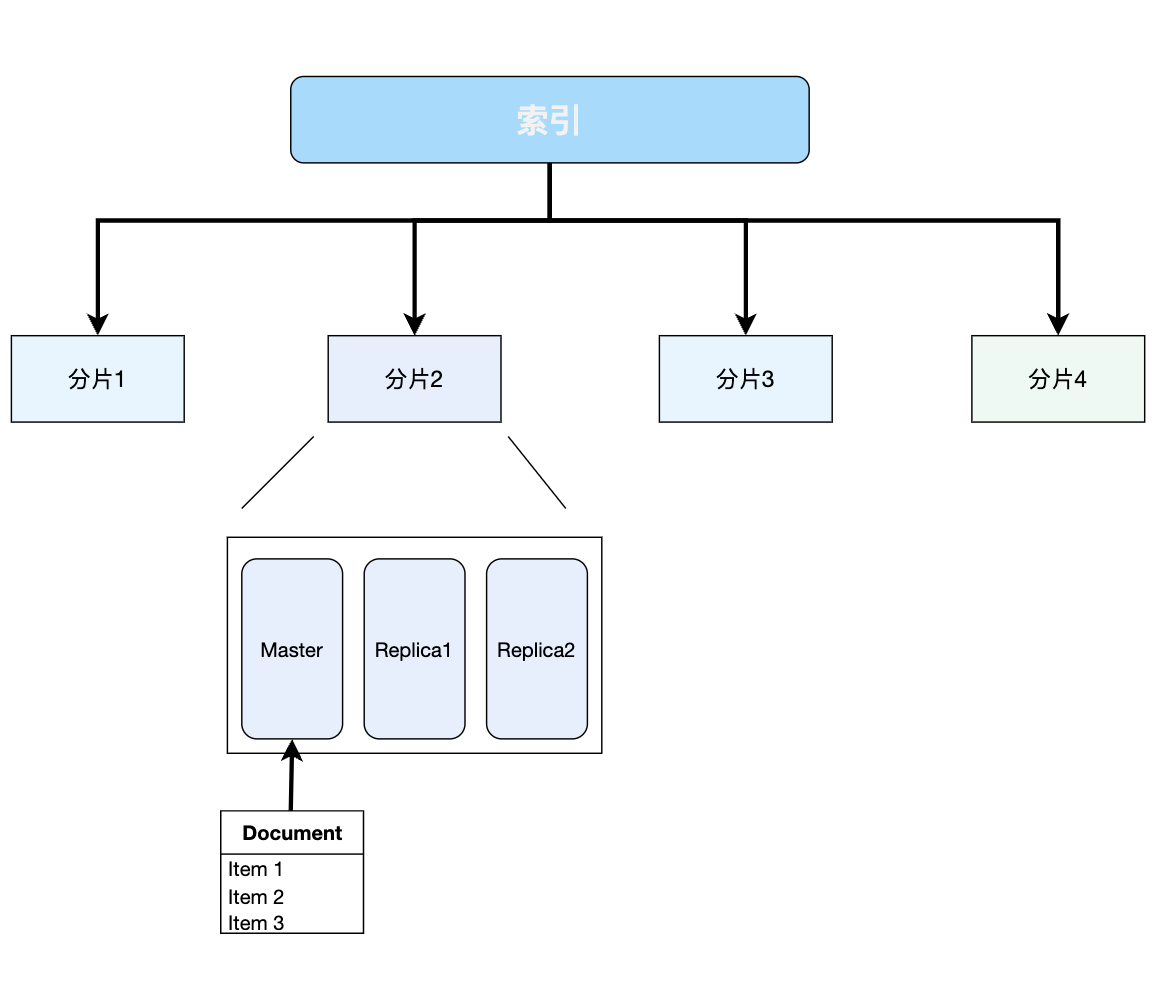
\includegraphics[width=0.95\textwidth]  {Elasticsearch.png}} 
	\caption{Elasticsearch结构}
	\label{es}
\end{figure}

如图\ref{es}所示,Elasticsearch 的集群由多个节点(Node)组成,每个节点可以承载一个或多个分片。集群中的数据以索引(Index)为单位进行组织,每个索引包含一组具有相似结构的文档(Document),并采用统一的映射(Mapping)进行管理。在多语言代码检索系统中,可以为不同的编程语言或项目类型分别建立索引,也可以将所有代码文件统一存储在一个索引中,便于统一检索和管理。需要注意的是,Elasticsearch 中的索引是逻辑上的数据集合,而分片则是物理上的数据分布单元。\par

为了实现分布式存储和提升系统的可用性与性能,Elasticsearch 引入了分片和副本的机制。每个索引可以被划分为多个主分片(Primary Shard),每个主分片又可以有一个或多个副本分片(Replica Shard)。主分片负责数据的写入和主控,副本分片则用于容错和负载均衡。当某个节点发生故障时,副本分片可以迅速接管,保证系统的高可用性和数据安全。在代码检索系统中,针对数百万个开源项目文件,可以通过合理配置分片和副本数量,优化系统的检索性能和容错能力。\par

文档(Document)是 Elasticsearch 中可被索引和检索的最小数据单元,采用 JSON 格式进行存储,类似于关系型数据库中的一行数据。在代码检索场景下,一个文档通常对应一个具体的代码文件,包含文件名、代码内容、开源协议、星数等丰富的元数据信息。通过灵活的映射配置,可以对不同类型的字段(如文本、数值、日期等)进行高效索引和检索。\par

此外,Elasticsearch 提供了功能强大的 RESTful API,便于与各类应用系统集成,并支持分布式部署、负载均衡、故障转移等企业级特性,保障系统的稳定性和可扩展性。Elasticsearch 内置了高效的全文检索、分词、聚合分析、排序和高亮显示等功能,支持多种复杂查询方式,包括关键词检索、布尔查询、短语匹配等。在代码检索系统中,可以结合代码结构化表达提取的特征进行索引,进一步提升检索的准确性和相关性。通过这些机制,Elasticsearch 能够高效地管理和组织大规模的代码数据,全面支持分布式、高并发的代码检索需求。\par
\subsection{Transformer驱动的大规模预训练语言模型}
\zihao{-4} 
大语言模型是实现本系统搜索功能的核心技术。近年来,随着代码数据规模的爆炸式增长,传统的基于关键词和规则的代码检索方法已难以满足开发者对语义理解和智能检索的需求。大语言模型凭借强大的语义建模和理解能力,能够对代码片段、函数、类等多粒度代码实体进行深层次的语义表示和推理,从而极大提升代码检索系统的智能化水平。当前,基于大语言模型的代码检索系统已成为智能开发辅助、代码推荐、自动补全等场景的关键基础设施。要深入理解当前的大语言模型,必须先了解其核心架构——Transformer。因此,本节将简要介绍Transformer及大语言模型的其他关键技术,并结合其在代码检索系统中的应用进行说明。

\subsubsection{Transformer}
Vaswani\cite{ref14}等人指出,循环神经网络模型(RNN)在每个时间步都需要依赖前一时间步的隐藏状态信息进行计算,这种固有的顺序依赖性使得RNN难以在多GPU上进行并行计算,从而限制了RNN在处理超大规模文本数据时的训练能力。为了解决这一问题,他们提出了Transformer架构,这是一种完全依赖注意力机制连接编码器和解码器的网络架构。Transformer显著提高了训练的并行度和速度。后续的一系列研究表明,基于Transformer架构的预训练模型(pre-trained models / pre-trained language models,PTM / PLM)在各种任务上都能实现最先进的性能表现,因此,Transformer已成为自然语言处理(NLP)领域的首选架构。除了在语言相关领域的应用之外,Transformer还被广泛应用于计算机视觉、音频处理以及自然科学学科,如化学、生物等领域。\par

\begin{figure}[H] 
	\center{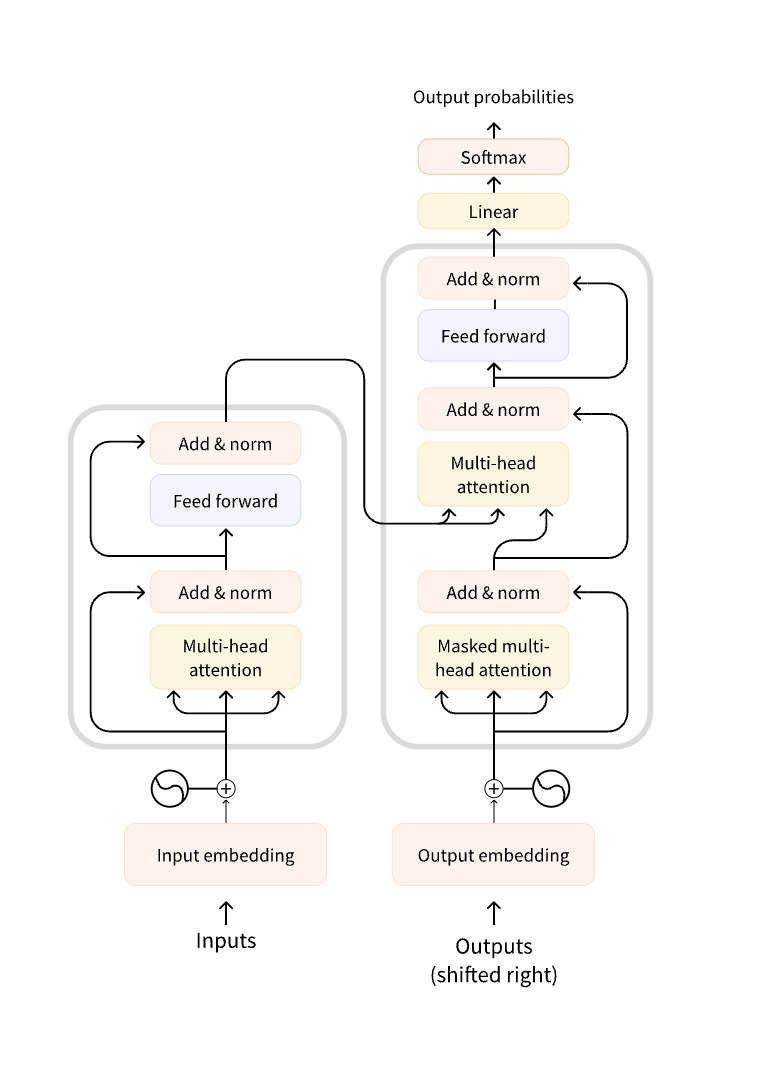
\includegraphics[width=0.95\textwidth]  {transformer.png}} 
	\caption{Transformer结构}
	\label{transformer}
\end{figure} %图表上下各空一行

Transformer架构如图\ref{transformer}所示,其整体由编码器(图\ref{transformer}左)和解码器(图\ref{transformer}右)组成。每个编码器块由多头注意力机制模块和位置前馈网络组成,模块间使用残差连接,并配有层归一化模块;解码器块在位置前馈网络和多头自注意力模块之间插入了交叉注意力模块,其中的自注意力模块用于组织某个位置信息对后续位置信息的影响。下面将简要介绍上述几种重要模块:\par
(1) 多头注意力机制:让序列中的每一个元素学习并计算与其他元素的互注意力分数权重,如公式\ref{func_1}所示:
\begin{eqnarray}
	\text{Attention(Q,K,V)} =  \text{softmax}(\frac{QK^T}{\sqrt[]{d_k}})V
	\label{func_1}
\end{eqnarray}
但Transformer并不只是简单应用了单个注意力函数,而是使用了多头注意力机制将 \(d_m\) 维度的原始 \(Q\)、\(K\)、\(V\) 分别线性投影到 \(d_k\)、\(d_k\)、\(d_v\) 维度,再根据公式\ref{func_1}进行注意力计算,整体公式如下:
\begin{eqnarray}
	\mathrm{MultiHead(Q,K,V)=~Concat(head_{1},...,head_{h})W^{O}} \\
	\mathrm{where~head_{i}~=~Attention(QW_{i}^{Q},KW_{i}^{K},VW_{i}^{V})}
	\label{func_2}
\end{eqnarray}
Transformer利用多头注意力机制能够同时关注到来自不同位置的且具有不同表示的子空间信息,增强了架构的表达能力。\par
(2) 位置前馈网络:全连接前馈网络模块,用于接收自注意力模块的输出:\par
\begin{eqnarray}
	\mathrm{FFN}(x) & =\max(0,x\mathrm{W}_1+\mathrm{b}_1)\mathrm{W}_2+\mathrm{b}_2 \\
	& =\mathrm{~ReLU(H'W}_1+\mathrm{b}_1)\mathrm{W}_2+\mathrm{b}_2
	\label{func_3}
\end{eqnarray}
(3) 残差连接与归一化:Transformer 在每个模块间使用残差连接,然后进行层归一化。其中编码器块表示为:\par
\begin{eqnarray}
	\mathrm{H^{\prime}=~LayerNorm(Self~Attention(X)+(X)} \\
	\mathrm{H=~LayerNorm(FFN(H^{\prime})+(H^{\prime})}
	\label{func_4}
\end{eqnarray}

\textbf{大语言模型与代码检索系统的关系:}  
基于Transformer的大规模预训练语言模型(如GPT、CodeBERT、Codex等)能够对自然语言查询和代码片段进行统一的语义建模,实现跨语言、跨风格的代码理解与检索。在代码检索系统中,大语言模型通常作为语义编码器,将用户的自然语言查询和代码库中的代码片段映射到同一语义空间,通过向量相似度检索相关代码。这种方法突破了传统基于关键词的检索方式,能够理解复杂的语义关系和上下文信息,显著提升了代码检索的准确率和智能化水平。此外,大语言模型还可用于代码摘要生成、代码补全、错误修复等多种智能开发场景,极大丰富了代码检索系统的功能边界。

\subsubsection{面向任务自适应的混合专家深度学习框架}
\begin{figure}[H]
	\center{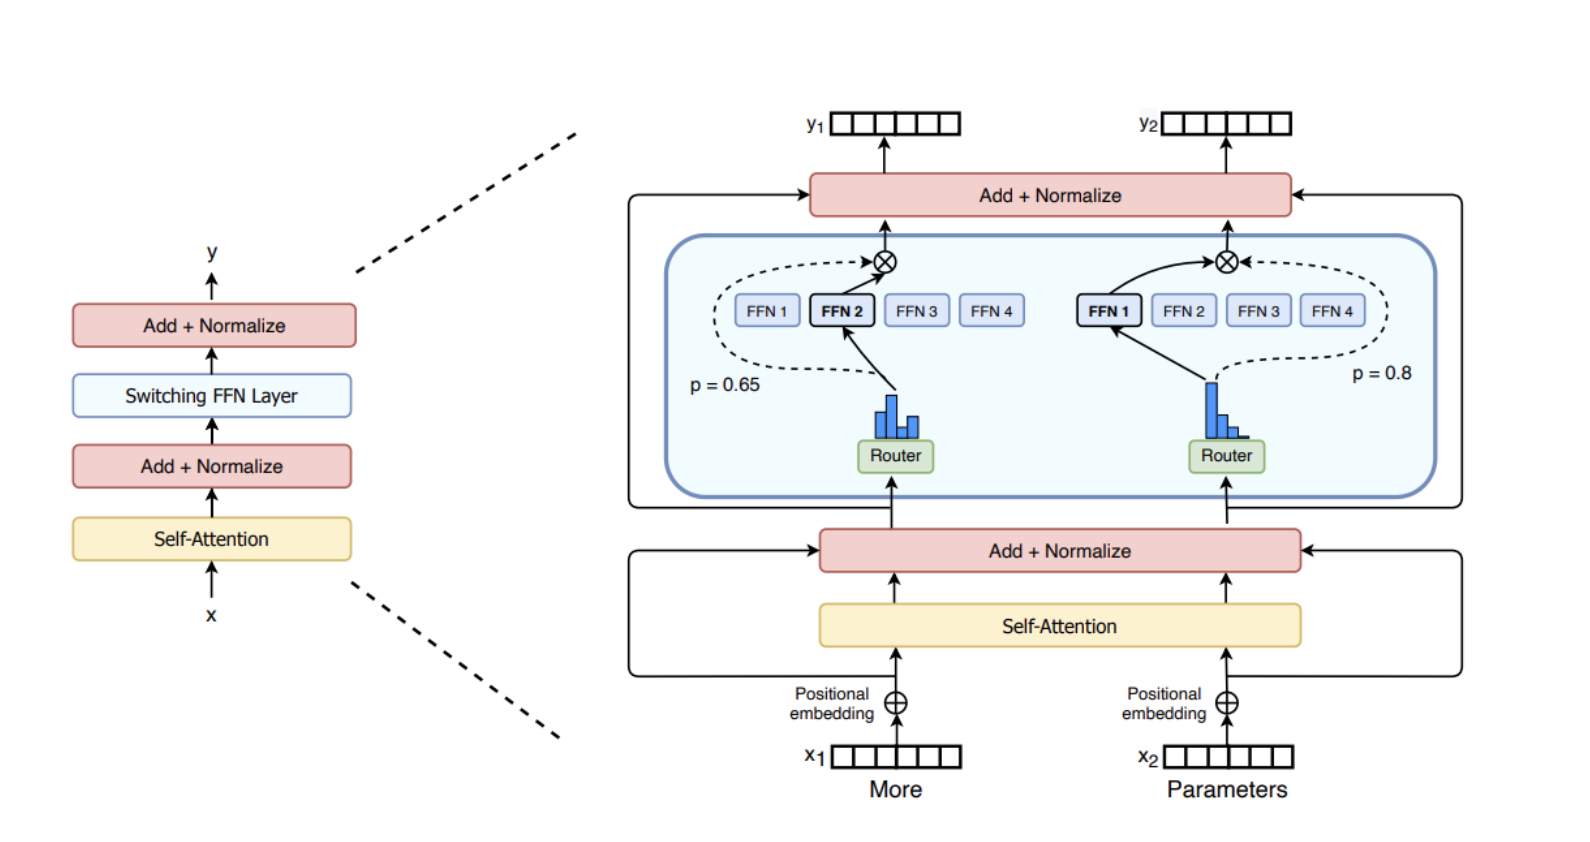
\includegraphics[width=0.95\textwidth]  {MoE.png}} 
	\caption{MoE结构}
	\label{MoE}
\end{figure}
Google Brain团队发现传统Transformer架构在扩展到超大规模时面临计算资源消耗激增的问题,尤其是前馈网络层(FFN)的全参数激活机制导致训练和推理效率急剧下降。为此,他们提出基于混合专家模型(Mixture of Experts, MoE)\cite{ref15}的稀疏架构改造方案,通过将Transformer中的FFN层替换为动态路由的专家网络集合,实现计算效率与模型容量的平衡。MoE架构如图\ref{MoE}所示,其核心创新在于引入稀疏门控机制(图\ref{MoE}蓝色部分),该机制由可学习的路由网络构成,针对每个输入词元生成专家选择概率分布,仅激活概率最高的前K个专家(通常K=2-4),其余专家保持非激活状态。具体而言,每个MoE层包含N个独立的前馈网络作为专家(例如N=8或32),其数学表达为:
\begin{eqnarray}
	\mathrm{MoE}(x)=\sum_{i=1}^KG(x)_i\cdot E_i(x)
	\label{func_5}
\end{eqnarray}
其中$G(x)$为门控网络输出的Top-K权重,$E_i(x)$为被选中的专家网络输出。这种设计使得模型总参数量可扩展至万亿级别,而实际计算量仅与激活专家数相关。实验表明,Switch Transformer在同等计算资源下,训练速度较传统稠密模型提升4倍,且推理时内存占用降低至1/4。进一步地,通过引入噪声注入(Noisy Top-K Gating)和负载均衡损失函数,MoE有效缓解了专家利用率不均衡问题,例如GLaM模型以1.2万亿参数仅激活97亿参数即达到GPT-3的97\%性能。当前,MoE架构已在GPT-4、DeepSeek、Mixtral 8x7B等主流大模型中广泛应用,成为突破单一模型规模瓶颈的核心技术路径。

\subsubsection{基于语义增强的大模型提示工程}
提示(Prompt)是一系列提供给大语言模型的指令,我们可以通过自定义提示来增强、改善大语言模型的能力。Schulhoff等人\cite{ref16}系统性地提出Prompt作为调控大型语言模型行为的核心接口,其本质是通过自然语言指令或结构化模板显式定义输入规范、处理规则及输出约束,从而动态重构大语言模型的上下文推理路径以适配特定任务需求。比如,可以指定大语言模型在生成文档时标记重点内容;可以指定大语言模型只输出符合要求的关键词语;可以指定大语言模型只生成指定代码风格的代码等。\par

提示工程(Prompt Engineering)作为一种独特的编程模式,主要围绕向大型语言模型精准输入提示展开操作。本质上,这一过程需要精心设计适配的提示模板,以此助力完成特定的下游任务。实践表明,优化提示内容能够显著提升模型在各类任务中的表现。\par

\begin{figure}[H]
	\center{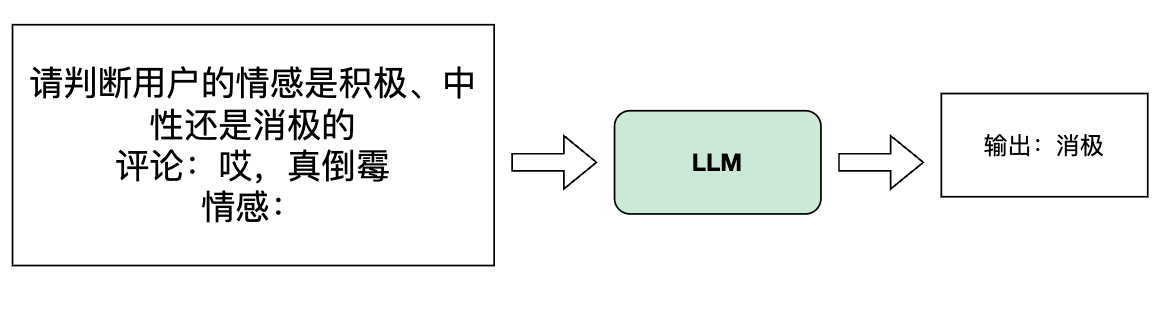
\includegraphics[width=0.95\textwidth]  {zero_shot.png}}
	\caption{零样本提示示例}
	\label{zero_shot}
\end{figure}
\begin{figure}[H]
	\center{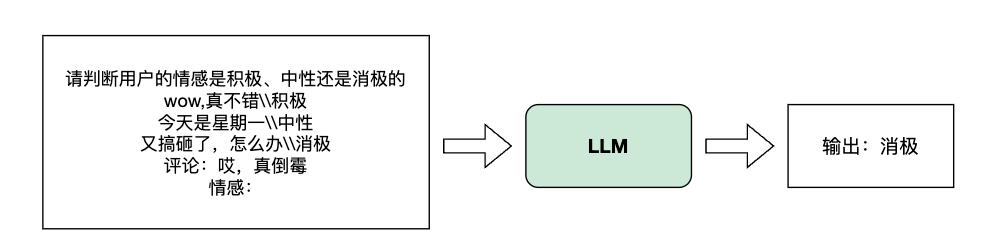
\includegraphics[width=0.95\textwidth]  {few_shot.png}}
	\caption{少样本提示示例}
	\label{few_shot}
\end{figure}
在提示工程的实际应用中,零样本提示(Zero-Shot Prompting)\cite{ref17}是一种基础方法,图\ref{zero_shot}展示了相关示例。该方法下,即便不向模型提供任何参考示例,模型也能够给出有价值的回应,完成既定任务。然而,当零样本提示无法满足需求时,少样本提示(Few-Shot Prompting)\cite{ref18}便派上用场,如图\ref{few_shot}。此时,需针对下游任务设计专门的提示模板,模板不仅要囊括一系列大语言模型处理规则,还要为后续待输入文本预留特定位置。在向大语言模型发起询问时,只需将待输入文本填充至提示模板预留空位,即可构建完整提示。除此之外,开启思维链、给大语言模型指定角色性格等提示技巧都能显著改变大语言模型输出效果和对任务的执行情况。\par
进一步看,巧妙构建提示能够催生全新的交互模式。借助提示指令,大语言模型可生成与软件工程概念相关的测验题目,模拟程序运行流程,甚至模拟命令行终端窗口的交互场景。不仅如此,提示还具备自适应特性,部分提示能够依据当前情况,推荐其他提示,以便收集更多信息,或生成相关成果物。提示的这些进阶功能,充分彰显了深入设计提示、挖掘其在简单文本与代码生成之外价值的重要意义。\par
在代码检索系统中,提示工程不仅可以用于优化自然语言查询的表达方式,还能引导大语言模型更好地理解用户意图,实现更为精准的代码匹配。通过设计针对代码风格、功能描述、编程语言等维度的提示,可以让大语言模型在检索和生成代码时更加贴合实际开发需求。此外,提示工程还可用于多轮对话、代码解释、错误定位等场景,提升代码检索系统的人机交互体验和智能化水平。
\subsection{基于微服务的高可用后台架构}
\zihao{-4}
微服务架构是本系统实现的核心技术之一,与微服务相对应的是传统的单体架构方案。单体架构(如图\ref{compare}左所示)将整个系统封装在一个程序中,集成了登录、鉴权、业务逻辑、数据处理等所有功能模块。这种“大而全”的架构对于小型系统而言,能够缩短开发周期,且开发和部署流程相对简单,符合开发者的直觉和习惯。然而,随着系统规模的扩大和业务复杂度的提升,单体架构逐渐暴露出模块耦合度高、扩展性差、维护成本高等问题,难以满足高并发、大数据量和多语言支持等现代应用场景的需求。\par
相比之下,微服务架构采用了“高内聚、低耦合”的设计理念,将系统的各个功能模块拆分为独立的服务,每个服务专注于完成某一特定功能,并以单独的进程或容器形式运行。整个系统由一组相互协作的微服务构成,服务之间通过网络进行通信(如图\ref{compare}右所示)。微服务架构的核心特点在于服务的颗粒度更细,职责更加单一,便于独立开发、测试、部署和扩展。通常情况下,每个微服务会运行在 Docker 容器中,而 Kubernetes 则负责对这些服务进行高效的管理和编排。通过这种方式,微服务架构不仅提升了系统的灵活性和可扩展性,还为大型复杂系统的开发和维护提供了更强的支持。\par

\begin{figure}[H]
	\center{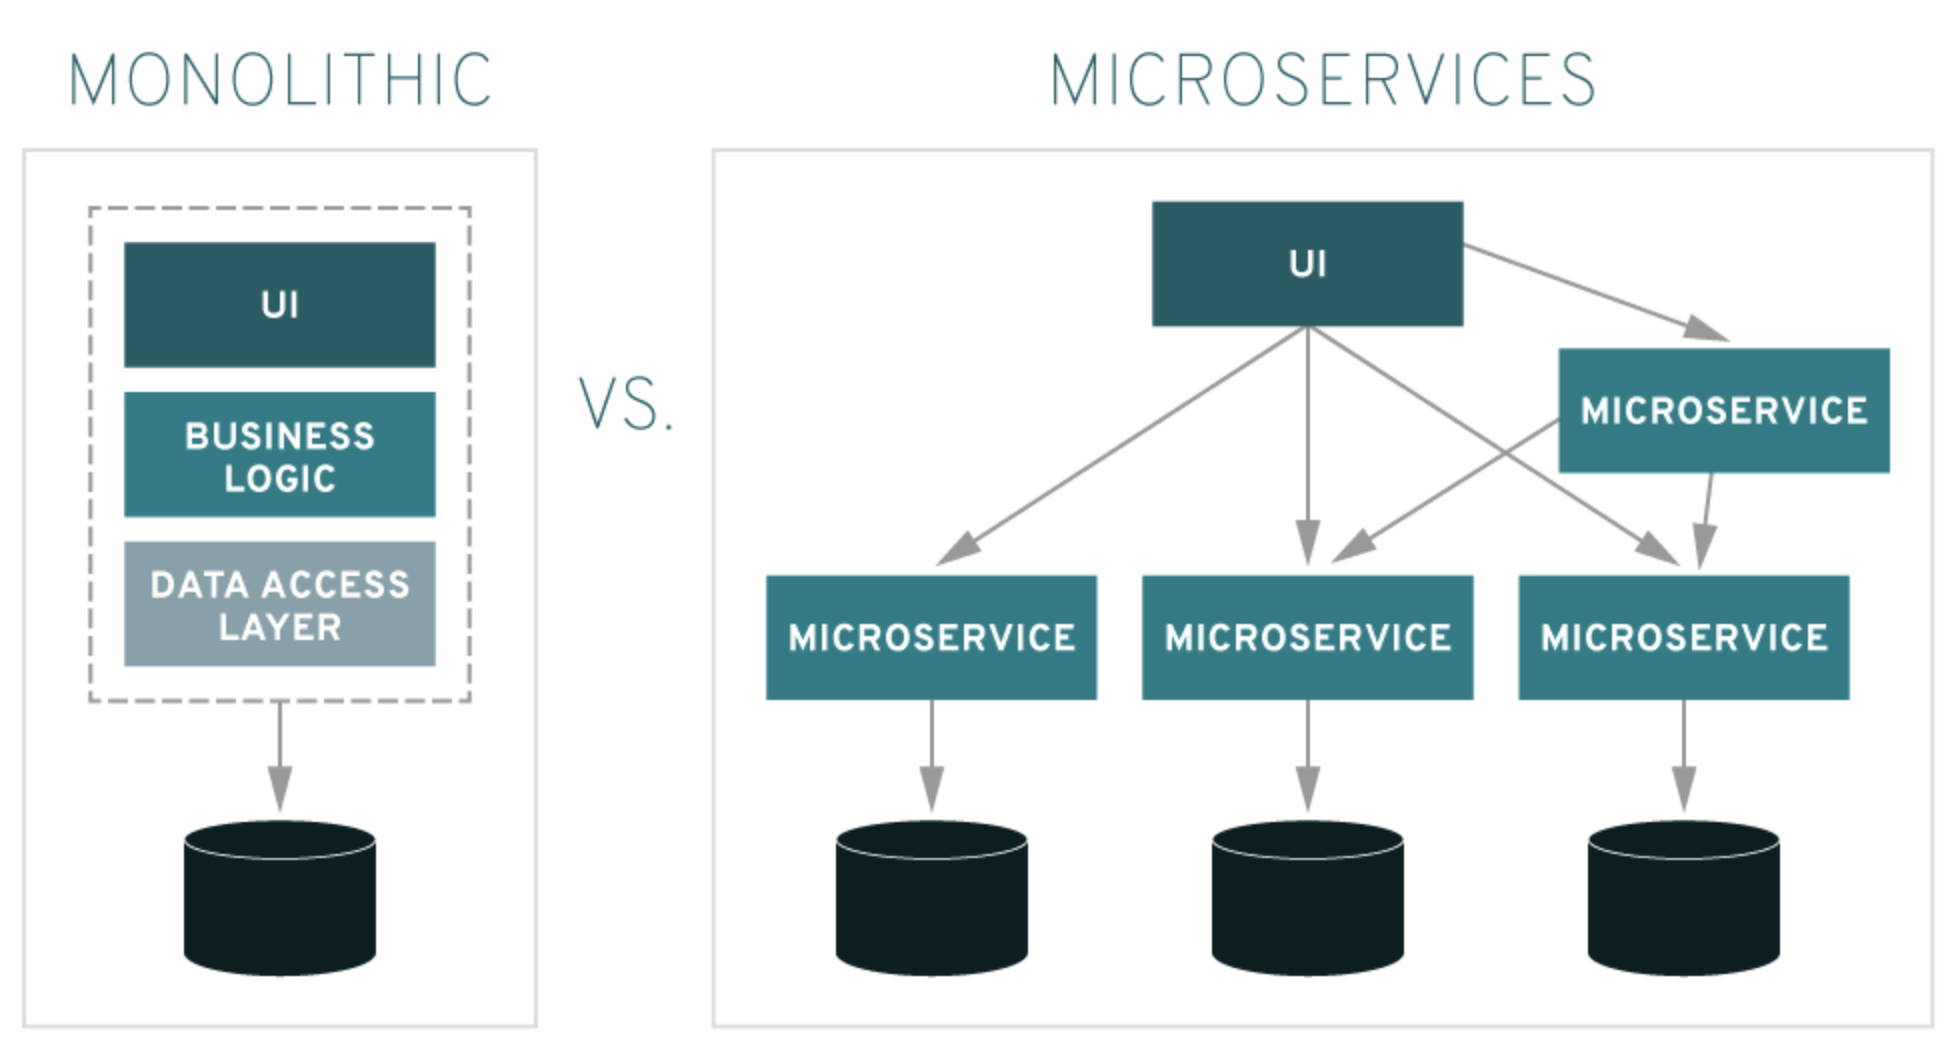
\includegraphics[width=0.95\textwidth]  {compare.png}} 
	\caption{单体架构和微服务架构对比}
	\label{compare}
\end{figure}
对于构建面向多编程语言的代码检索系统而言,系统通常需要处理多种编程语言的解析、索引、检索、语义分析等复杂任务,同时还需要依赖大模型实现检索词的检索增强功能。不同编程语言的处理逻辑、依赖环境和扩展需求各不相同,单体架构难以灵活应对多语言场景下的异构需求。但是对于微服务而言,每个微服务可以采用最适合其功能的编程语言和技术栈。例如可以使用Python服务部署大语言模型,实现系统中的检索增强功能,使用Go语言搭建的网关、鉴权、检索等服务可以应对高并发的请求处理,以及业务的安全校验。这样不仅提升了开发效率,也方便集成社区已有的多语言处理工具。同时针对不同模块的微服务而言,可以独立扩展相关微服务的实例数,实现资源的动态分配和弹性伸缩。比如对于网关这类的服务而言,往往是IO密集型而非CPU密集型,因此在部署的时候可以考虑使用轻量级的容器实例进行横向扩展,以应对高并发的网络请求压力;而对于大语言模型推理服务,则通常是计算密集型任务,可以部署在具备GPU加速能力的节点上,并根据实际负载动态调整模型服务的副本数,从而实现资源的高效利用和系统整体的弹性伸缩。此外,微服务架构还支持服务的独立升级与灰度发布。当需要对某一编程语言的解析模块进行功能优化或安全加固时,只需对对应的微服务进行迭代和部署,无需影响其他服务的正常运行。这种解耦的架构极大降低了系统维护和演进的复杂度,提升了系统的可维护性和可用性。在多语言代码检索系统中,微服务架构还便于集成和管理多种第三方工具与智能组件。例如,可以为不同编程语言分别集成专用的语法分析器、静态检查工具或代码格式化服务,也可以灵活接入多种大语言模型用于语义增强、代码补全或自然语言查询理解。各服务之间通过gRPC等高效协议进行通信,保证了系统的高性能和低延迟。\par
因此,微服务架构为面向多编程语言的代码检索系统提供了高可用、高扩展性和高灵活性的基础设施保障,是支撑大规模、智能化代码检索服务的关键技术路径。\par

\subsubsection{跨语言的远程调用框架}
gRPC是一种高性能、开源的跨语言远程过程调用(RPC)框架,广泛应用于微服务架构下的服务间通信。gRPC\cite{ref19}允许客户端应用程序直接调用服务器端应用的方法,就像它们是本地对象一样,这使得分布式应用程序开发变得更加容易。gRPC使用HTTP/2作为传输协议,支持双向流、头部压缩等特性,从而提供了更高效的网络通信。此外,gRPC通过Protocol Buffers定义接口和服务,这是一种轻量级、跨平台的消息格式,有助于提高数据交换效率并减少带宽使用。在微服务架构中,gRPC因其高效性而被广泛用于服务间通信。\par
在gRPC中,服务定义和数据交换格式通常使用Protocol Buffers。Protocol Buffers是由Google设计的一种轻量级、跨平台的消息格式,用于序列化结构化数据。通过.proto文件,开发者可以定义自己的数据结构和服务接口。这些定义被编译成不同编程语言的代码,以便生成易于使用的类来构建强类型的请求和响应消息。与其他序列化协议(如JSON、XML、BSON等)相比,protobuf采用二进制编码,消息体积小,传输高效,适合高并发和大数据量场景。除此之外,protobuf支持多种编程语言,gRPC自带的编译工具可快速生成多语言桩代码,适合多语言协作的微服务架构。并且protobuf通过为字段分配唯一标识符,支持消息格式的平滑演进,保障了系统的长期可维护性。

\subsubsection{容器化部署与环境隔离基础设施}
Docker\cite{ref20}是一个开源的应用容器引擎,使开发者可以将应用程序及其依赖打包到一个可移植的容器中,然后发布到任何流行的Linux或Windows机器上,也可以实现虚拟化。容器采用沙箱机制,彼此隔离,安全性高。Docker容器的轻量化和快速部署能力使其成为微服务架构中的理想选择。每一个微服务都可以被打包成一个独立的Docker容器,确保了环境一致性,简化了开发、测试和部署流程。同时,由于Docker容器的资源消耗低,多个容器可以在同一台物理机上高效共存,提高了资源利用率。Docker采用联合文件系统(Union File System)技术,将不同的文件系统层叠加在一起,形成统一视图。每个Docker镜像由一系列只读层组成,创建容器时会在最顶层添加一个可写层。层次化设计不仅加快了镜像构建和分发过程,还提升了数据隔离性和安全性(如图\ref{docker})。\par
\begin{figure}[H]
	\center{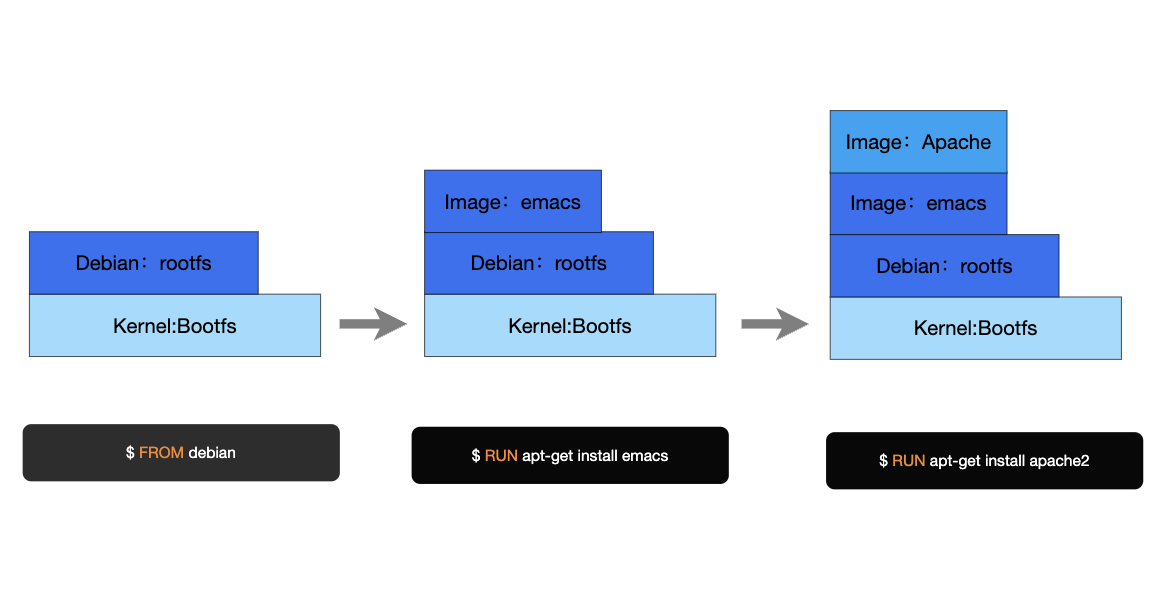
\includegraphics[width=0.95\textwidth]  {docker.png}} 
	\caption{docker层次化构建示例}
	\label{docker}
\end{figure}
\subsection{本章小结}
\zihao{-4} 
本章介绍了实现面向多编程语言的代码检索系统的核心理论和技术。首先介绍了代码检索问题的基本内涵及其在现代软件工程中的重要意义,分析了代码结构化表达对于实现跨语言、深层次代码理解与检索的基础作用。随后,详细阐述了分布式高性能搜索引擎在大规模代码数据管理与高并发检索中的应用优势,为系统的可扩展性和高可用性提供了有力支撑。在智能检索层面,重点解析了以Transformer为代表的大规模预训练语言模型的原理及其在代码语义建模、跨语言检索等场景中的应用价值。进一步介绍了混合专家模型等前沿深度学习架构在提升模型容量与推理效率方面的创新,以及基于提示工程的语义增强方法对大语言模型能力的优化和扩展。通过这些技术,系统能够实现对自然语言查询和多语言代码的统一语义理解,显著提升检索的准确性和智能化水平。在系统架构方面,论述了微服务架构在多语言代码检索系统中的关键作用。微服务通过服务解耦、异构技术栈支持、弹性伸缩和高可用性,极大提升了系统的灵活性和可维护性。结合gRPC、Docker等云原生技术,实现了高效的服务通信、环境一致性,满足了大规模、复杂业务场景下的高并发和持续演进需求。综上,本章为后续系统设计与实现奠定了坚实的理论基础和技术支撑,明确了多语言代码检索领域的研究趋势与技术挑战,为构建高效、智能、可扩展的代码检索平台提供了全面的指导和参考。
\newpage
\fancyhead[LH]{\zihao{-5}{\songti 重庆大学本科学生毕业论文(设计)}}
\fancyhead[RH]{\zihao{-5}{\songti 3\quad 系统需求分析与设计实现}}
\section{面向多编程语言的代码检索系统需求与设计}
\subsection{用户需求}
在本系统的设计与开发过程中,用户需求分析始终是需求工程的核心和基础。面向多编程语言的代码检索系统,其目标用户群体主要涵盖了软件开发者、编程学习者等多类人群。通过对不同用户实际使用场景的梳理,可以发现他们对代码检索系统的需求具有一定的共性,也存在各自的侧重点。以软件开发者为例,在日常开发过程中,尤其是在实现标准业务模块或者需要完成某些特定功能时,经常会遇到需要参考行业最佳实践或标准实现方式的情况。例如,开发者在接入某个数据库时,可能需要查找该数据库在不同编程语言下的SDK接入示例;或者在实现分布式系统时,想要了解某种语言下CAS锁的标准写法;又或者在实现轮询器、消息队列等通用组件时,希望能够借鉴社区中成熟的代码片段。这些场景下,开发者往往希望能够快速检索到高质量、可复用的代码实现,减少重复造轮子的时间和精力。而对于编程学习者来说,代码检索系统的主要用途则体现在学习和练习过程中,比如在刷算法题、完成课程作业或自学新技术时,遇到难以独立实现的功能,便希望通过检索系统查找相关的代码片段进行参考和学习,从而加深对知识点的理解和掌握。\par
具体到功能层面,用户普遍希望能够通过自然语言描述或者简洁的关键词输入,快速定位到与自身需求高度相关的代码片段或完整项目实现。由于实际开发和学习过程中涉及的编程语言种类繁多,用户往往需要跨语言、跨项目地查找解决方案,因此系统必须具备多编程语言的检索能力,并能够根据用户输入自动识别目标语言、相关API、开源协议等关键信息。检索结果的展示方式也非常重要,用户希望系统能够以直观、结构化的界面呈现检索结果,便于快速浏览和对比不同的实现方案。对于感兴趣的代码片段,用户还希望能够进一步查看其所属项目的详细信息,包括项目描述、开源协议、星标数量、文件结构等,以便综合评估代码的可用性、合规性和维护性。此外,部分用户尤其是开发者群体,还希望能够将检索到的代码片段直接集成到本地开发环境中,或者通过VS Code插件实现一键插入和复用,进一步提升开发效率和体验。\par
\begin{figure}[H]
	\center{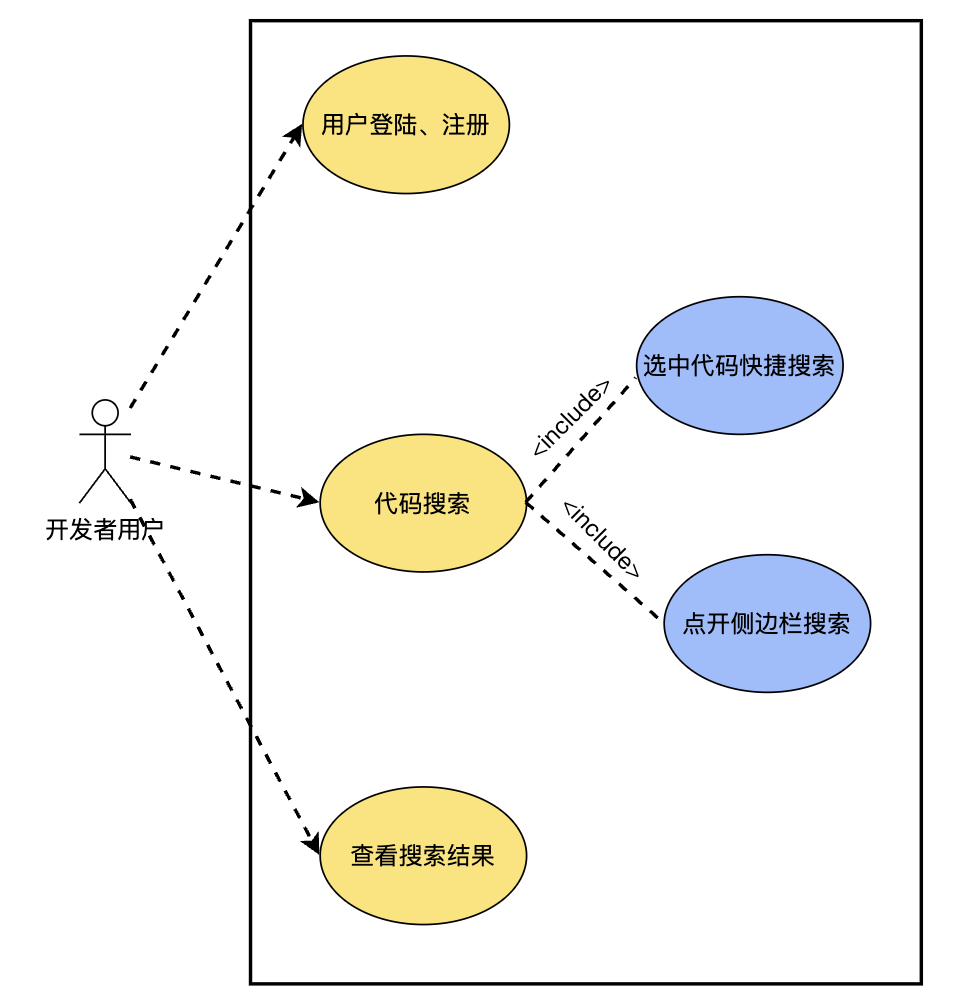
\includegraphics[width=0.85\textwidth]{user_use.png}}
	\caption{面向多编程语言的代码检索系统用户用例图}
	\label{usecase}
\end{figure}
在用户权限和数据安全方面,用户普遍关注个人信息和检索历史的安全性与隐私性,因此希望系统能够提供完善的注册、登录和身份认证机制,防止未授权访问和数据泄露。综合上述分析,本文通过用例图,如图\ref{usecase}所示,对主要用户需求进行了建模,涵盖了代码检索、项目详情查看、用户注册与登录、权限管理等核心用例。每个用例均对应具体的用户操作流程和系统响应,确保需求分析的完整性和可追溯性,为后续系统设计和实现提供了坚实的基础。\par
\subsection{功能需求}
基于对用户需求的深入分析,面向多编程语言的代码检索系统需要实现一系列核心功能,以支撑用户在多语言、多场景下的高效代码检索与复用。主要功能需求包括但不限于以下几个方面:\par
(1)系统应具备强大的代码检索功能。用户可以通过自然语言描述、关键词输入或代码片段示例,发起多编程语言的代码检索请求。系统需支持对主流编程语言(如Python、Java、Go、C++、JavaScript等)的代码片段、函数、类、模块等多粒度对象的检索,并能够根据用户输入自动识别目标语言、相关API、开源协议等信息。检索功能应支持模糊查询、精确匹配、语义扩展等多种检索模式,提升检索的灵活性和准确性。\par
(2)系统应支持项目详情查看功能。对于每个检索到的代码片段,用户可以进一步查看其所属项目的详细信息,包括项目名称、描述、开源协议、星标数量、文件结构、原始链接等。系统应支持对项目文件的层级浏览和快速定位,便于用户深入分析项目实现和依赖关系。此外,在用户管理与权限控制方面,系统应提供完善的用户注册、登录、身份认证和会话管理功能。支持用户信息的安全存储与加密传输,防止未授权访问和数据泄露。\par
(3)系统应支持VS Code插件集成。用户可以通过VS Code侧边栏或快捷键,直接在本地开发环境中发起代码检索、预览和插入操作,实现Web端与本地端的无缝协同,极大提升开发效率和用户体验。\par
\subsection{非功能需求}
除了上述核心功能需求外,面向多编程语言的代码检索系统还需满足一系列非功能性需求,以保障系统的高可用性、可扩展性和用户体验。主要非功能需求包括以下几个方面:\par
(1)系统应具备良好的性能表现。在高并发访问场景下,系统应能够在秒级内响应用户的检索请求,确保检索结果的实时性和交互的流畅性。为此,系统后端需采用高性能的分布式查询引擎,并结合缓存、异步处理等优化手段,提升整体吞吐量和并发处理能力。对于大规模代码数据集,系统应支持分布式存储与索引,确保数据的高效管理和快速检索。\par
(2)系统应具备良好的可扩展性。随着用户规模和数据量的不断增长,系统应能够通过横向扩展(如增加服务器节点、微服务实例等)实现弹性扩容,避免单点瓶颈和性能瓶颈。系统架构应采用微服务化设计,各服务单元可独立部署、升级和扩展,便于后续功能迭代和技术演进。\par
(3)系统应具备高可用性和容错能力。为保障系统在高并发、分布式部署和节点故障等复杂场景下的稳定运行,系统应引入服务注册与发现、负载均衡、健康检查、自动故障转移等机制,确保部分节点故障时系统整体仍能正常服务。对于核心数据和服务,系统应支持多副本备份和自动恢复,提升系统的鲁棒性和可靠性。\par
(4)系统应支持多端一致性和跨平台兼容性。无论用户通过Web端还是VS Code插件访问系统,均应获得一致的功能体验和界面风格。系统前端应适配主流浏览器和操作系统,后端应支持多种开发环境和部署平台,提升系统的适用范围和用户覆盖面。\par
\subsection{其他需求}
在功能和非功能需求之外,面向多编程语言的代码检索系统还需关注安全性、可维护性、易用性等其他关键需求,以提升系统的综合竞争力和用户满意度。系统的安全性需求至关重要。系统应采用HTTPS协议加密所有前后端通信,防止数据在传输过程中被窃取或篡改。用户密码等敏感信息应采用哈希加密存储,防止数据库泄露带来的安全风险。系统应实现完善的身份认证与权限校验机制,防止未授权访问和会话劫持等安全威胁。其次,系统的可维护性需求体现在架构设计、代码规范和文档完善等方面。系统应采用分层、模块化的架构设计,各功能模块职责清晰、接口标准,便于后续的功能扩展和技术升级。系统代码应遵循统一的编码规范和注释标准,提升代码的可读性和可维护性。另外,系统的易用性需求直接影响用户的使用体验,系统界面应简洁直观,操作流程清晰,对于新用户,系统应提供友好的注册、登录和引导流程,降低上手门槛。此外,系统还应遵循相关的开源协议和数据使用规范,尊重原作者的知识产权和数据隐私。\par
\subsection{系统总体架构设计}
面向多编程语言的代码检索系统整体将采用前后端分离的方式进行组织。可以分为前端交互层、后端逻辑层以及数据层三个维度,如图\ref{all_structure}所示。前端交互层使用Vue框架编写交互逻辑,使用ElementUI渲染前端图形化页面和可视化模块。后端使用Gin框架结合gRPC框架编写应用服务,规范API风格,接受前端请求,同时负责和数据层和大语言模型进行交互,实现主要的搜索逻辑。数据层使用Elasticsearch管理所有的项目数据。
\begin{figure}[H]
	\center{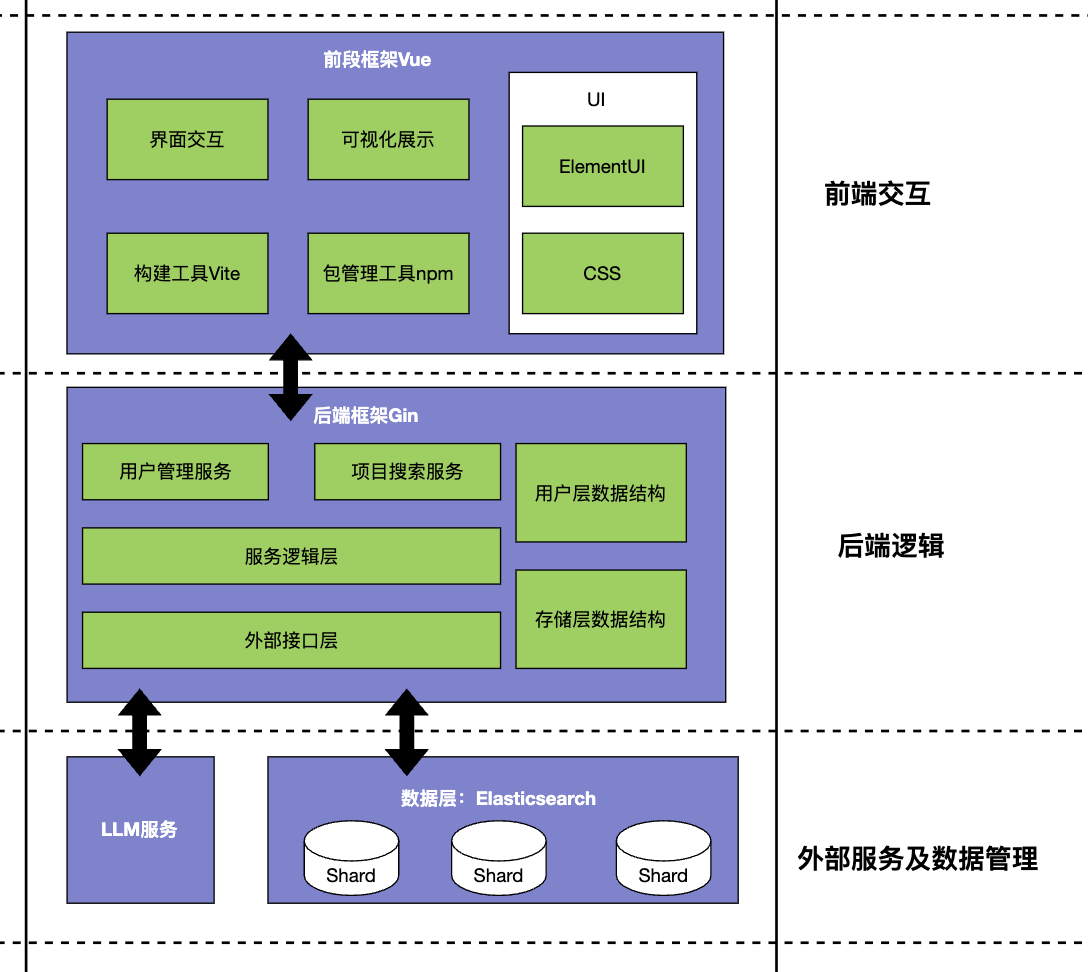
\includegraphics[width=0.95\textwidth]  {structure.png}} 
	\caption{系统总体架构图}
	\label{all_structure}
\end{figure}
\subsection{基于AST的代码结构化预处理设计}
代码结构化表达方式是指将源代码从原始的文本形式转化为能够反映其语法结构和语义信息的形式化表示。与普通文本不同,源代码具有严格的语法规则和层次化的结构,单纯依赖表层的字符串匹配难以捕捉代码的深层含义。因此,如何对代码进行结构化建模,是实现高效、准确代码检索和理解的基础。在软件工程的实践中,我们通常会用到AST这样的静态分析手段来对代码进行结构化的表达。\par
AST是代码结构化表示中最常用的方法之一。AST以树状结构描述源代码的语法结构,将代码分解为语法单元,并以节点的形式组织起来。通过AST,可以有效捕捉代码的层次关系和语法特征,便于后续的代码分析、转换和检索。通常抽象语法树以代码中的条件判断分支作为树的节点,之所以说AST是抽象的因为树上的每一个节点不代表任何一种具体语言的具体条件控制语句,仅代表节点本身所映射的条件控制逻辑,例如“如果”,“循环”等。\par
\begin{figure}[H]
	\center{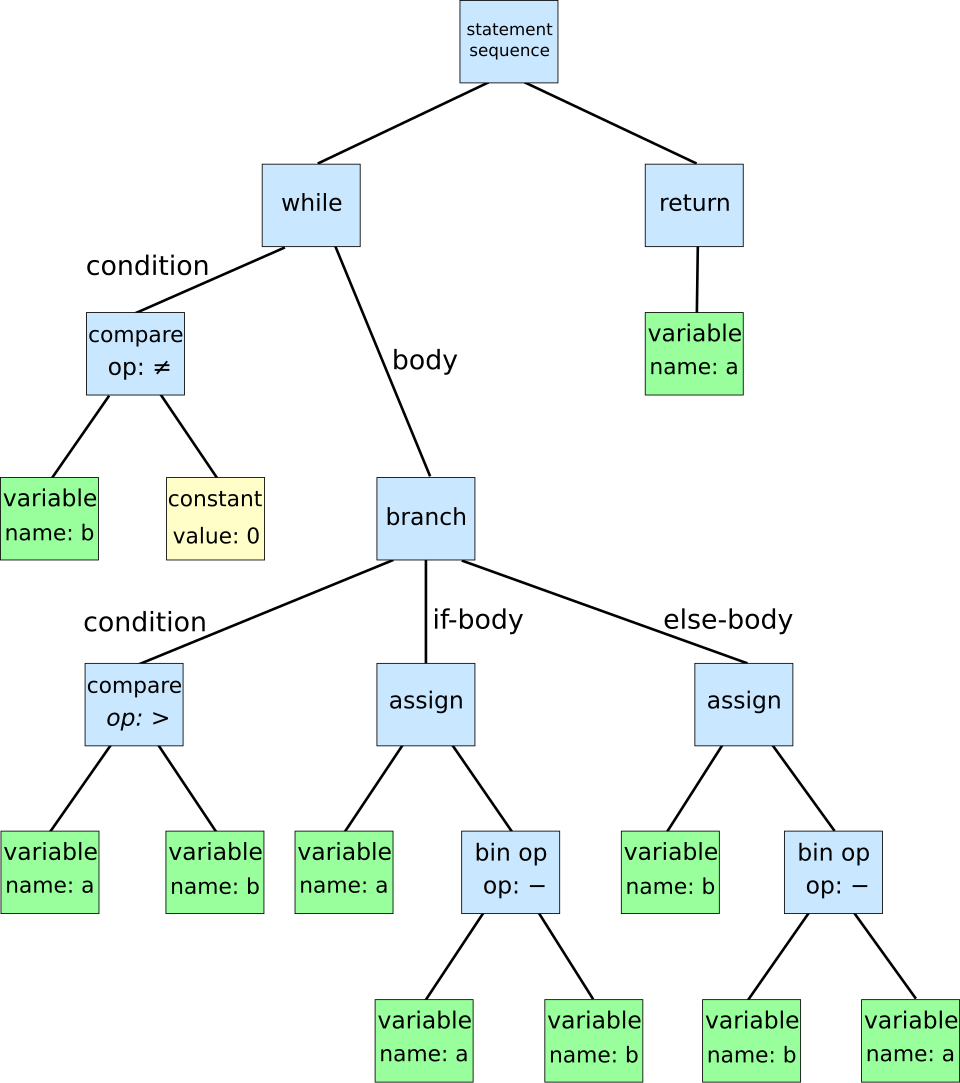
\includegraphics[width=0.95\textwidth]  {ast.svg.png}} 
	\caption{抽象语法树示例}
	\label{ast}
\end{figure}
一个常见的语法树如图\ref{ast}所示,图中的“while”,“compare”都表示实际代码中的具体控制逻辑,但是该抽象语法树并未映射任何语言。通过抽象语法树,能够高效的分析出代码的具体的控制结构。由于AST本质上是一种抽象的语法表示,不依赖于具体编程语言的语法细节。通过对不同语言的AST进行归一化处理,可以实现跨语言的结构对齐和统一建模,为多语言代码检索和迁移提供基础。由于大部分的代码结构都较为规范,因此使用AST能够很好的适配较多数的代码。并且由于AST采用树状图的结构对代码进行分析,能够便于对代码的层次关系和控制结构进行分析。基于AST可以实现对完整项目的具体拆解,使得代码搜索的颗粒度得到细化,能够有助于代码检索系统实现跨语言搜索的特性。为此,本文拟采用主流的开源AST解析工具,对不同编程语言的项目源代码进行统一的结构化预处理。通过AST分析,可以有效揭示代码的层次结构与语义关系,为后续的特征提取和检索任务提供坚实的数据基础。\par
本项目中,代码预处理拟分为三个阶段:\par
(1)在代码收集阶段,系统通过自动化工具从开源代码托管平台批量抓取多种编程语言的代码仓库。为了保证数据的多样性和代表性,收集范围涵盖了主流编程语言如Java、Python、Go、JavaScript等,同时优先选择活跃度高、星标数量多的项目,以确保代码质量和实用价值。自动化脚本定期执行,能够持续更新和扩充代码库,满足系统对大规模、多语言代码数据的需求。收集过程中,系统还对仓库的元信息进行抓取,包括项目描述、开源协议、贡献者信息等,为后续的检索和筛选提供辅助数据支持。\par
(2)在结构化处理阶段,系统针对不同编程语言调用对应的开源AST解析工具,对收集到的源代码进行语法分析,自动生成抽象语法树。该过程是为了实现了代码的统一结构化表达,以便于跨语言的语义对齐和特征抽取。系统对生成的AST进行遍历和筛选,剔除无关的冗余信息,如注释、单元测试代码及无实际业务逻辑的辅助函数,仅保留核心功能实现相关的代码片段。为了提升数据的一致性和可比性,系统将对AST节点进行规范化处理,包括统一节点类型命名、变量和函数标识符等。通过这一阶段的处理,原始代码被转化为结构清晰、语义明确的中间表示,以便为后续的语义理解和检索提供坚实的基础。\par
(3)在分析与存储阶段,系统将对结构化处理后的代码数据进行质量评估和统计分析,以判断代码收集和预处理是否符合预期要求。通过自动化脚本对代码的覆盖率、功能模块分布、语言比例等关键指标进行监控,及时发现可能存在的数据偏差或异常情况,确保数据集的完整性和代表性。符合质量标准的结构化代码及其对应的项目元信息将被统一存储于Elasticsearch数据库中,以支持高效的索引和检索。该数据库不仅保存代码的文本内容,还包含丰富的结构化信息,如函数签名、调用关系和代码注释等,有助于提升检索的准确性和响应效率。\par
\begin{figure}[H]
	\center{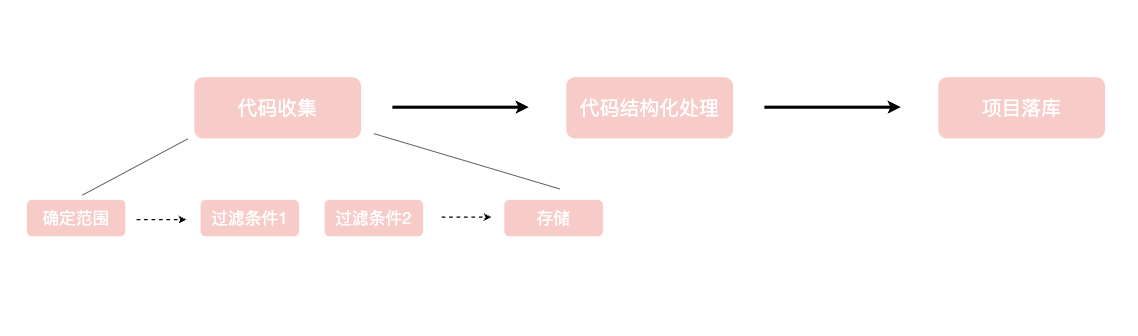
\includegraphics[width=0.95\textwidth]{pre_pro.png}}
	\caption{基于AST的代码结构化预处理设计}
	\label{pre_pro}
\end{figure}
总体而言,代码的结构化预处理过程如图\ref{pre_pro}所示,基于AST的代码结构化预处理流程旨在实现从代码采集、结构化转换到数据存储的闭环管理,为多编程语言代码检索系统提供高质量、结构化的基础数据支持。\par
\subsection{基于微服务的高可用后台分布式设计}
随着软件系统规模的不断扩大和业务复杂度的持续提升,传统的单体式后端架构已难以满足现代多编程语言代码检索系统在高可用性、可扩展性和灵活性方面的需求。微服务架构作为当前主流的分布式系统设计范式,通过将复杂系统拆分为一组松耦合、自治的服务单元,实现了服务的独立部署、弹性扩容和高效协作,成为支撑大规模智能代码检索平台的关键技术基础。所谓微服务架构,是指将系统按照业务功能划分为多个独立的服务,每个服务围绕特定业务能力构建,拥有独立的数据存储和运行环境,并通过轻量级通信机制(本文使用gRPC协议)进行协作。与传统单体架构相比,微服务架构不仅提升了系统的可维护性和可演化性,还极大增强了系统在高并发、分布式部署和多语言支持等场景下的适应能力。在面向多编程语言的代码检索系统中,微服务架构能够有效支撑多语言解析、智能检索、权限管理等异构服务的协同运行,为系统的高可用性和弹性扩展提供坚实保障。\par
本节围绕高可用后台分布式技术的微服务架构展开,提出了一套系统化的后端设计方案。该方案以服务自治、弹性伸缩和容错机制为核心,结合分布式服务注册与发现、负载均衡、服务治理等关键技术,实现了多编程语言代码检索系统的高可用、可扩展和易维护的后端支撑平台。整体方案包括以下两个阶段:\par
(1)第一阶段为服务拆分与分布式部署。系统根据业务功能将后端划分为网关服务、鉴权服务、搜索服务、大语言模型服务等多个微服务单元。每个服务均可独立开发、测试、部署和扩容,极大提升了系统的灵活性和可维护性。通过容器化技术和分布式编排平台,各服务能够在多节点环境下弹性部署,实现资源的动态调度和高可用保障。服务间通过gRPC等高效通信协议进行数据交互,确保低延迟和高吞吐量。\par
(2)第二阶段为高可用性与服务治理机制设计。系统引入分布式服务注册与发现机制,所有微服务在启动时自动向服务注册中心,注册自身信息,其他服务可通过注册中心动态发现并调用目标服务,提升系统的灵活性和容错能力。为应对高并发和突发流量,系统在网关层集成负载均衡策略,自动分发请求至后端多实例服务,避免单点瓶颈。各服务内部实现健康检查与自动故障转移机制,确保部分节点故障时系统整体仍能稳定运行。此外,系统还支持灰度发布、自动扩缩容、日志追踪与链路监控等服务治理能力,为后续功能迭代和运维管理提供有力支撑。\par
\begin{figure}[H]
	\center{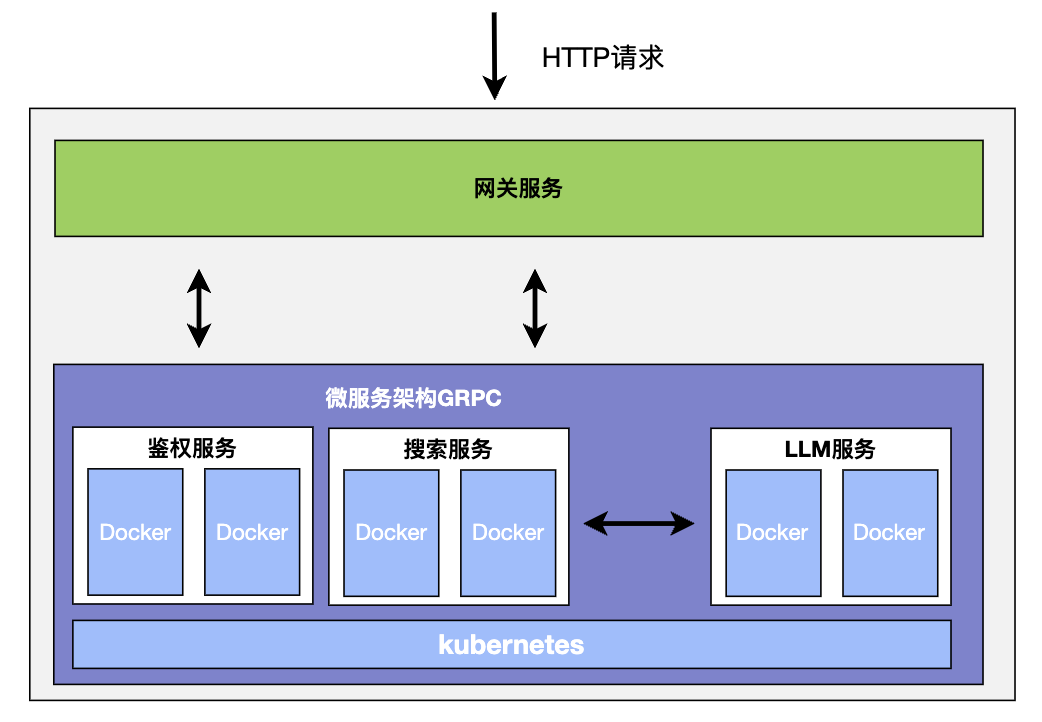
\includegraphics[width=0.95\textwidth]{back_model.png}}
	\caption{微服务架构下的高可用分布式后台结构}
	\label{microservice_arch}
\end{figure}
如图\ref{microservice_arch}所示,为面向多编程语言的代码检索系统的整体后台架构。网关统一对外提供API入口,负责请求路由、鉴权与负载均衡。鉴权服务独立负责用户注册、登录与Token校验,保障系统安全。搜索服务与大语言模型服务协同,实现多语言代码的查询上下文增强以及智能检索。所有服务均支持多实例部署,结合容器编排平台实现弹性扩容和自动恢复,显著地提升系统的高可用性和并发处理能力。\par
\subsection{基于提示词工程的查询上下文增强技术}
随着大语言模型在自然语言处理和代码智能领域的广泛应用,提示词工程逐渐成为提升模型性能和用户体验的关键技术之一。所谓提示词工程,是指针对特定任务或应用场景,系统性地设计、优化和管理输入给大语言模型的提示,以引导模型生成更符合预期的输出结果。与传统的模型训练和微调方法不同,提示词工程无需对模型参数进行修改,而是通过调整输入内容和结构,充分挖掘和利用预训练模型的知识和推理能力。在基于大语言模型的多编程语言代码检索系统中,提示词的设计与优化对检索效果具有决定性影响。尤其是在处理跨语言、跨领域的复杂检索需求时,提示词不仅承担着任务指令的基本职责,更需要有效整合用户意图、上下文信息以及目标语言特性,从而提升模型对查询语义的理解能力和检索结果的相关性。本节围绕查询上下文增强的提示词工程展开,提出了一套系统化的提示词设计流程。该流程的核心在于以结构化上下文信息为中介桥梁,实现用户自然语言查询与多语言代码语料之间的高效对接。整体流程包括两个阶段:\par
第一阶段为查询意图解析与上下文信息提取。系统首先对用户输入的原始检索词进行语义分析,识别其中的功能需求、目标编程语言、相关API或库等关键信息。同时,结合用户历史检索记录、当前项目上下文等外部信息,自动补全或纠正不完整、模糊的查询表达。该阶段输出结构化的查询意图数据,为后续提示词生成提供事实性基础。\par
第二阶段为提示词模板生成与大模型推理。系统将解析得到的结构化查询意图与用户原始检索词一并输入,通过精心设计的提示词模板,引导大语言模型进行代码检索。该阶段的目标是融合用户需求、上下文信息与目标语言特性,提升模型对检索意图的理解深度和检索结果的准确性。\par
基于该分层式的提示词工程,设计查询语句的上下文增强技术,有望实现用户查询意图的精准解析与高效表达,充分发挥大语言模型的语义理解优势,为多编程语言代码检索系统提供强有力的模型支持,提升检索的准确性和用户体验。\par
\subsection{智能代码检索系统前端架构}
本系统前端交互界面采用基于Vue框架的MVVM(Model-View-ViewModel)架构模式,将整体结构划分为视图层(View)、视图模型层(ViewModel)和模型层(Model)三个部分。整体前端系统架构如图\ref{front_model}所示。
\begin{figure}[H]
	\center{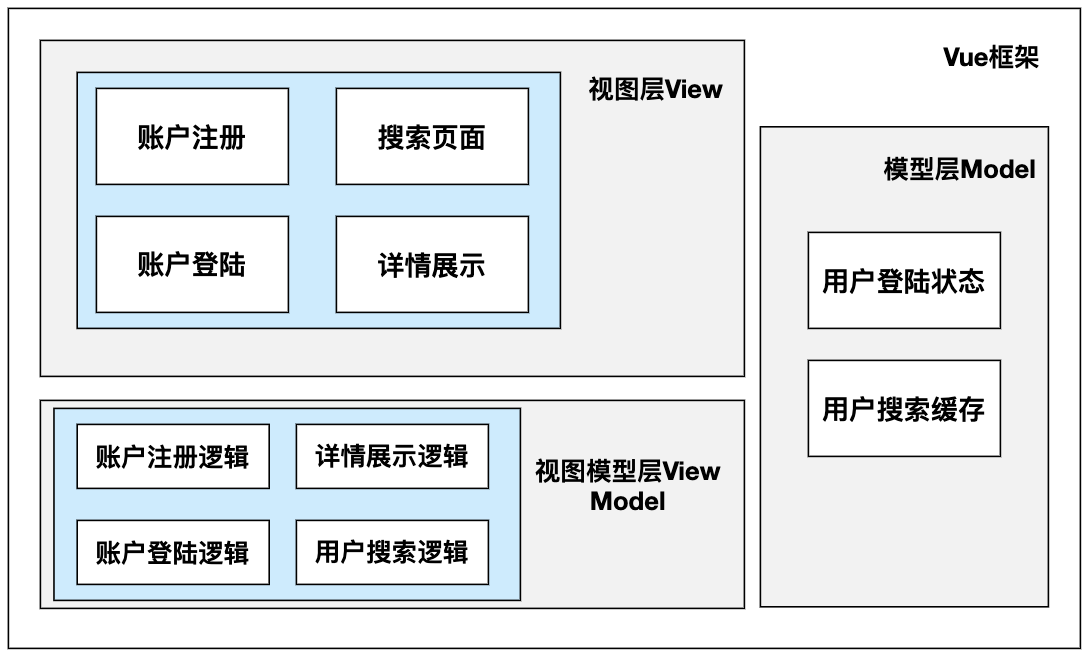
\includegraphics[width=0.95\textwidth]{front_model.png}}
	\caption{前端系统架构图}
	\label{front_model}
\end{figure}
视图层负责呈现用户界面,承载所有用户交互操作。主要包括开发者的注册与登录界面、代码检索页面、检索结果展示页面、用户个人中心及项目管理等功能模块。视图层通过Vue的组件化机制实现界面元素的复用与动态渲染,支持响应式设计以适配不同终端设备,提升用户体验的流畅性和一致性。\par
视图模型层作为视图层与模型层之间的桥梁,负责处理前端业务逻辑。该层实现了账户注册与登录的表单验证与状态管理、代码搜索请求的构造与发送、检索结果的分页与筛选、项目详情的动态展示等核心功能。视图模型层通过Vue的响应式数据绑定机制,实时监听用户操作并更新视图状态,确保界面与数据的同步。该层还负责调用后端API接口,处理异步请求与错误反馈,保障前后端交互的稳定性和高效性。\par
模型层主要用于前端数据的临时存储和状态管理。系统采用Vuex作为集中式状态管理工具,统一管理用户信息、检索历史、搜索结果及项目数据等关键状态。模型层通过对数据变化的监听与响应,实现跨组件的数据共享和状态同步,避免数据冗余和不一致问题。此外,模型层还支持本地缓存机制(如localStorage或IndexedDB),提升用户操作的连续性和离线体验。\par
为了提升系统的可维护性和扩展性,前端架构还引入了模块化开发和路由管理。通过Vue Router实现页面间的动态切换和权限控制,确保不同用户角色访问对应功能模块。组件之间通过事件机制和状态管理进行解耦,方便后续功能迭代和团队协作开发。
综上,本系统前端架构基于Vue MVVM模式,结合组件化、响应式数据绑定和集中式状态管理,构建了一个结构清晰、响应迅速且易于维护的智能代码检索用户界面,为用户提供流畅、高效的交互体验。
\subsection{本章小结}
本章系统性地阐述了面向多编程语言的代码检索系统的需求分析与方案设计,涵盖了从用户需求到技术实现的全方位内容。通过详尽的用户需求调研,明确了系统需支持多编程语言、多场景下的高效代码检索,满足开发者和学习者对代码片段、项目详情及跨语言查询的多样化需求,同时强调了安全性和权限管理的重要性。基于此,提出了系统的功能需求和非功能需求,涵盖强大的检索能力、项目详情展示、VS Code插件集成、高性能响应、可扩展性及高可用性等关键指标。在方案设计层面,系统采用前后端分离架构,前端基于Vue MVVM模式构建响应式、模块化的交互界面,支持多端一致体验和状态管理;后端则基于微服务架构实现高可用分布式部署,结合服务注册发现、负载均衡和容错机制,保障系统的稳定性和弹性扩展。数据层通过基于AST的代码结构化预处理,实现多语言代码的统一表示和高质量索引,提升语义理解和检索精度。综上,本章构建了一个架构合理、功能完备的多编程语言智能代码检索系统方案,为后续的系统实现与优化奠定了坚实基础,确保系统能够高效满足用户多样化需求,提升代码检索水平和用户体验。\par
\section{面向多编程语言的代码检索系统方案实现}
\subsection{基于AST的编程语言预处理实现}
在本系统的预处理阶段,针对不同编程语言,设计并实现了基于抽象语法树(AST)的代码结构化处理模块。该模块主要依托于多种开源AST解析器,如Go语言的\texttt{go/ast}包、Python的\texttt{ast}模块以及Java的\texttt{JavaParser}等,能够自动对多语言项目的源代码进行语法分析,生成对应的抽象语法树。系统通过统一的接口封装不同语言的解析工具,实现了对多语言代码的统一处理流程,保证了预处理过程的可扩展性和灵活性。\par
\begin{figure}[H]
	\center{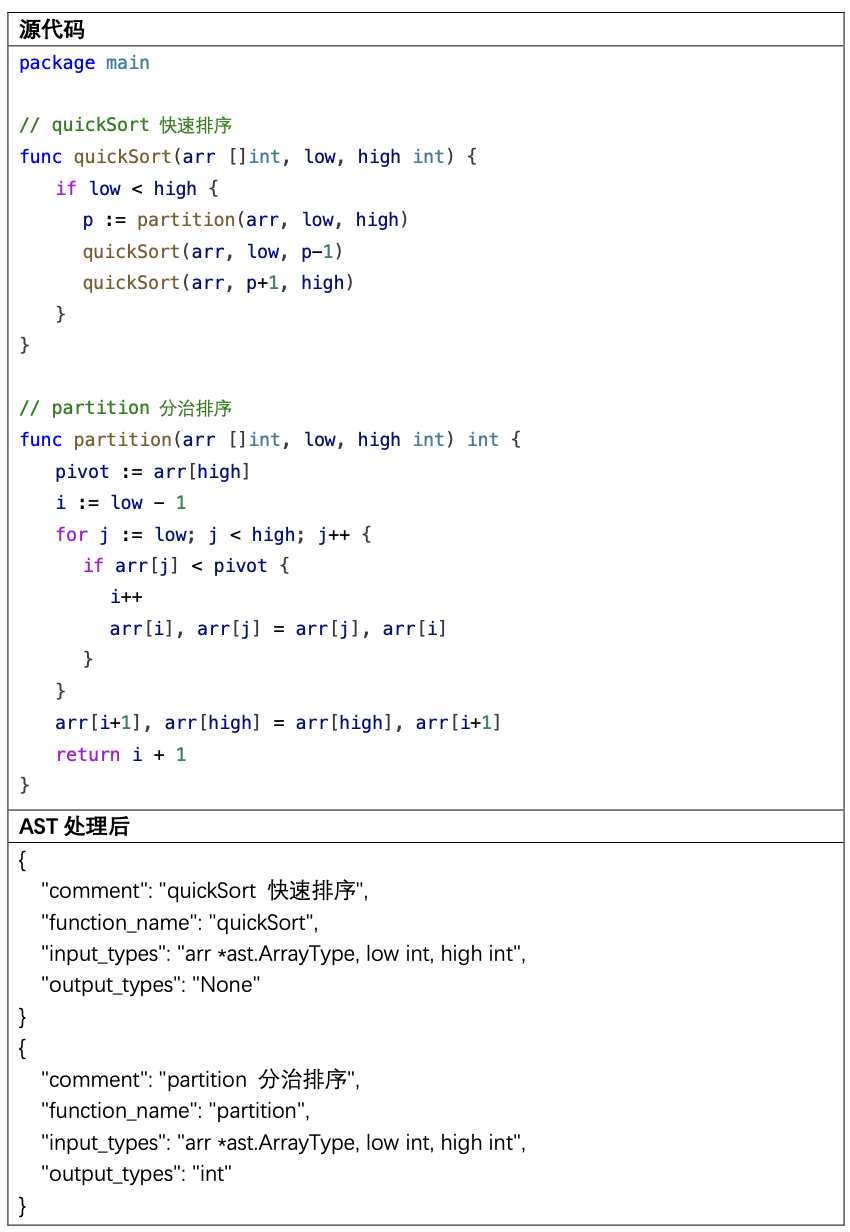
\includegraphics[width=0.95\textwidth]  {ast_example.png}} 
	\caption{AST处理示例图}
	\label{ast_example}
\end{figure}
系统首先对收集到的代码仓库进行遍历,针对每个文件调用对应语言的AST解析器,自动生成完整的语法树结构。随后,系统对生成的AST进行深度遍历,筛选出与核心业务逻辑相关的代码节点,自动剔除注释、单元测试代码以及无实际功能的辅助代码片段。此步骤有效提升了数据集的纯净度,避免了无关信息对后续检索模型的干扰。为了进一步增强数据的一致性和跨语言对齐能力,系统对保留的功能函数进行了结构化处理,包括统一节点类型的命名规范,以及对变量名和函数标识符的标准化处理,减少了不同语言间的命名差异对检索效果的影响。\par
如图\ref{ast_example}所示,系统以一段Go语言实现的快速排序代码为例,经过AST处理后,去除了具体的递归实现细节,仅保留了函数名、注释信息以及方法的输入输出类型等关键信息,极大地规范了代码的存储格式。该处理不仅保证了代码结构的完整性,也为后续的语义分析和跨语言检索提供了高质量的输入数据。通过该预处理模块,系统能够有效地将多语言源代码转化为统一且结构化的中间表示,显著提升了代码检索的准确性和效率。整体来看,基于AST的预处理实现为多编程语言代码检索系统奠定了坚实的基础,确保了后续检索服务能够在多语言环境下高效运行。\par
\subsection{基于微服务的高可用后台分布式技术实现}
\subsubsection{微服务系统中的统一接入与安全网关服务}
在基于微服务的分布式系统中,服务网关是保证整体服务安全、可扩展性与高可用性的核心基础设施之一。所谓服务网关,是指在分布式微服务系统中,作为所有外部请求的统一入口,负责流量调度、统一鉴权、安全防护、协议转换等多重关键任务。与传统单体系统的直接访问模式不同,服务网关通过集中管理和智能路由,有效屏蔽了后端服务的复杂性,提升了系统的安全性、灵活性和运维效率。在面向多编程语言的代码检索系统中,网关机制不仅承担着请求分发和安全防护的基本职责,更需要适应多语言、多协议和高并发的复杂业务场景,从而保障系统整体的稳定运行和高效服务能力。\par
\begin{figure}[H]
	\center{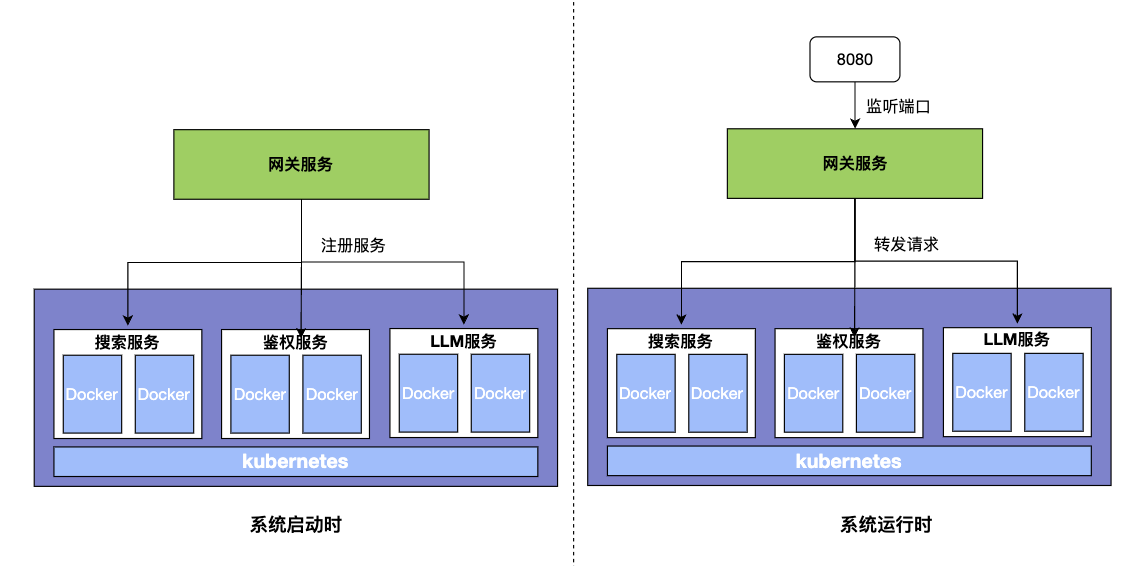
\includegraphics[width=0.95\textwidth]  {gateway.png}} 
	\caption{网关工作原理图}
	\label{gateway}
\end{figure}
在面向多编程语言的代码检索系统中,网关服务基于Gin框架,基本实现了服务的统一注册,均衡路由以及服务鉴权等功能。图\ref{gateway}为本服务的网关服务的简单工作原理图示例。网关的工作过程分为服务启动时和服务运行时两个阶段。在在服务启动时,网关会向鉴权服务、搜索服务和大语言模型服务发送探活请求,确保系统内所有服务都能够正常连接。在服务运行时,网关服务监听服务器的特定端口。在本系统中,网关监听8080端口,所有的请求经过网关集成的多种负载均衡策略(如轮询、最少连接等)之一,根据实时流量和服务健康状态,智能分发至后端对应的微服务实例。同时,对于所有的请求,都将经过鉴权服务鉴权,确保请求访问的权限在安全控制范围呢。\par
\subsubsection{微服务系统中的统一身份认证与安全鉴权服务}
在现代微服务系统中,统一身份认证与安全鉴权机制是保障系统安全性、数据完整性与用户隐私的核心基础设施。所谓鉴权服务,是指在多服务协同的分布式系统中,专门负责用户身份验证、权限校验及会话管理的独立服务模块。与传统单体系统中嵌入式的认证方式不同,分布式鉴权系统通过集中式管理和标准化接口,有效提升了系统的安全性、可扩展性和运维效率,并且往往依赖分布式数据库解决统一路由问题。在面向多编程语言的代码检索系统中,鉴权服务不仅承担着用户注册、登录与会话管理的基本职责,更需适应高并发环境下的复杂业务场景,从而为系统的安全运行和用户体验提供坚实保障。
\begin{figure}[H]
	\center{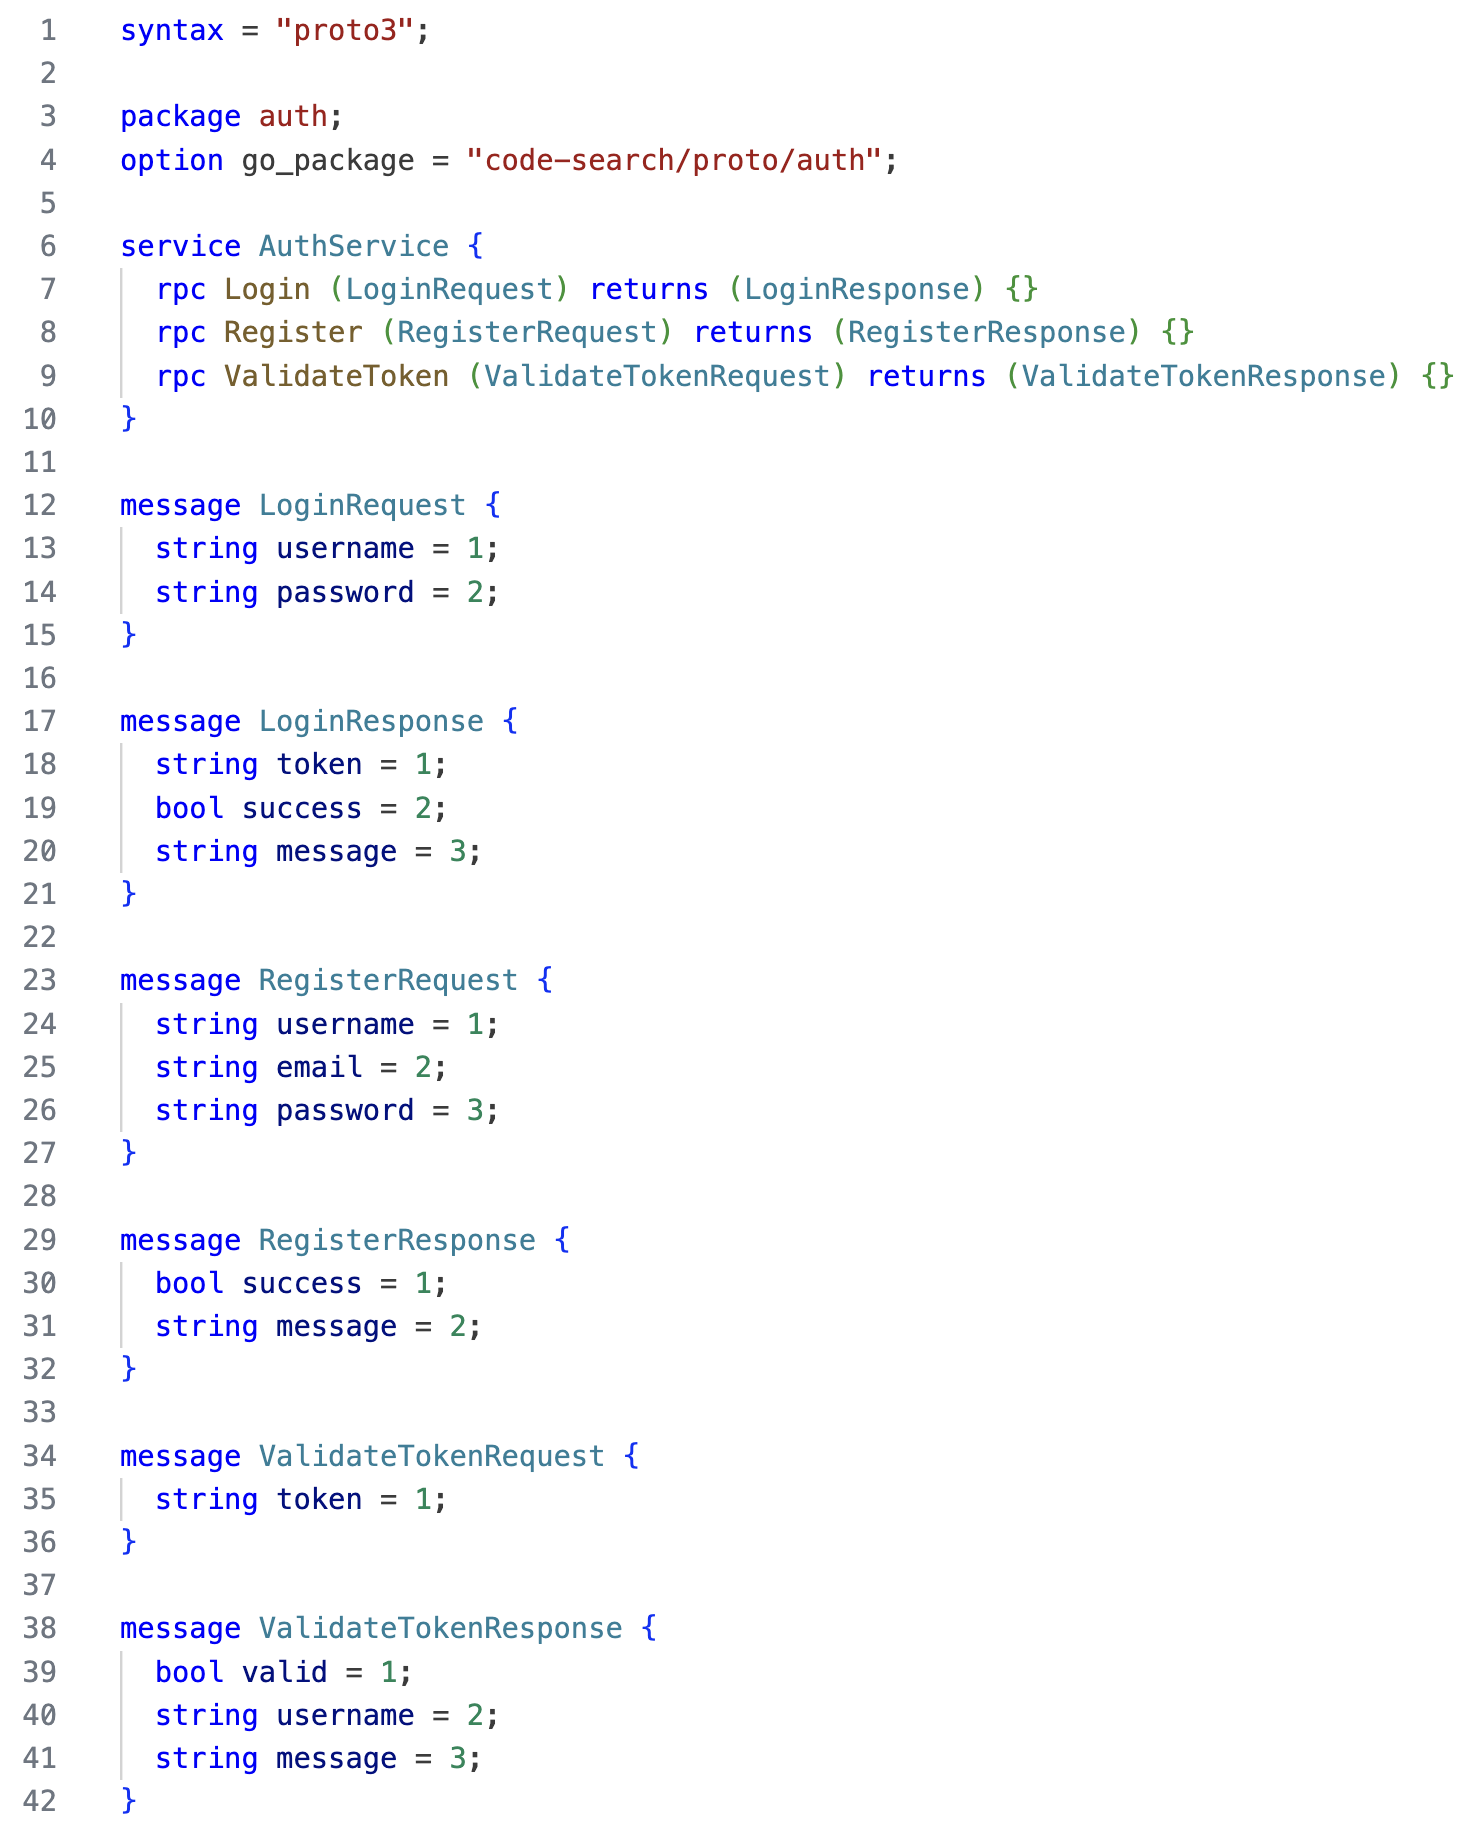
\includegraphics[width=0.95\textwidth]  {proto.png}} 
	\caption{鉴权服务协议}
	\label{auth}
\end{figure}
本系统的统一身份认证与安全鉴权机制基于gRPC高性能通信框架实现,采用标准化的proto协议(如图\ref{auth}所示)定义服务接口,确保各微服务间的高效互操作与安全通信。整体流程涵盖用户注册、登录认证与会话状态校验等核心环节,如图\ref{auth_flow}所示,具体包括以下三个阶段:\par
\begin{figure}[H]
	\center{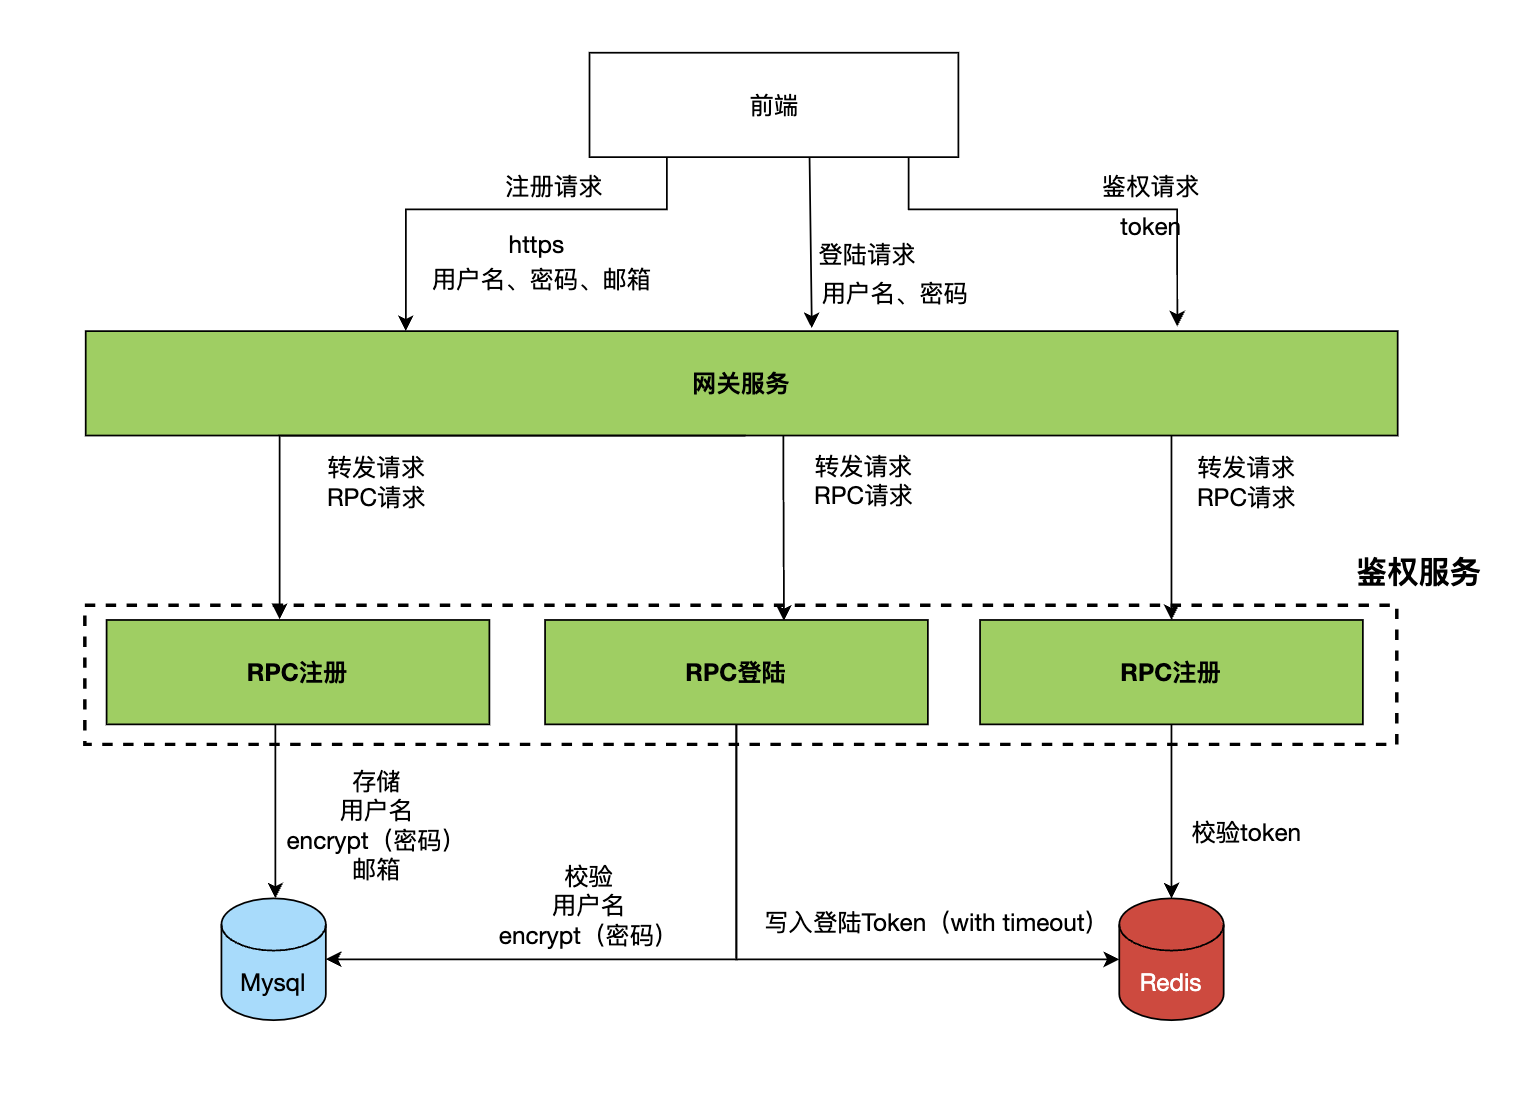
\includegraphics[width=0.95\textwidth]{auth.png}}
	\caption{统一身份认证与鉴权服务工作原理}
	\label{auth_flow}
\end{figure}
第一阶段为用户注册与身份信息安全存储。用户通过前端界面提交用户名、邮箱及密码等注册信息,所有注册请求均通过HTTPS协议加密传输至服务网关,从而防止敏感数据在传输过程中被窃取。服务网关对请求进行初步校验后,将其转发至鉴权服务的注册接口。为进一步保障用户密码安全,系统采用哈希加密算法对密码进行不可逆处理,最终将加密后的密码存储于数据库中。即使数据库遭受攻击,用户的原始密码信息也无法被直接获取,有效提升了系统的抗攻击能力。用户注册信息表如表\ref{usertable}所示,其中id字段作为用户的唯一标识符,由系统使用雪花算法自动生成。雪花算法是一种高效且广泛认可的ID生成方案,能够在本项目的用户基数和并发量下充分保证ID的唯一性。用户名(username)、电子邮件(email)及密码(password)字段则用于用户的注册和认证过程,且密码在存储前均经过哈希加密处理,从而在数据传输和存储环节进一步保障了用户信息的安全性。\par
\begin{table}[H]
	\centering
	\caption{用户信息表(code\_search\_user)}
	\small
	\begin{tabular}{c c c c}
		\toprule
		列名 & 数据类型 & 主键 & 注释\\
		\midrule
		id & bigint & 是 & 用户ID(通过雪花算法自动生成)\\
		username & varchar(255) & 否 & 用户名\\
		email & varchar(255) & 否 & 用户电子邮件地址\\
		password & varchar(255) & 否 & 用户密码(采用哈希加密存储)\\
		\bottomrule
	\end{tabular}
	\label{usertable}
\end{table}
第二阶段为用户登录与会话令牌(Token)分发。用户通过输入用户名和密码发起登录请求,系统在接收到请求后,对用户提交的凭证进行哈希校验。认证通过后,鉴权服务为用户生成唯一的会话Token,并将该Token安全存储于分布式Redis集群中。此后,用户在访问系统各项服务时,均需携带该Token以证明其身份合法性。Token机制不仅提升了系统的安全性,还便于实现分布式环境下的无状态会话管理。\par
第三阶段为会话状态检测与权限校验。每当用户发起请求时,需在请求头中携带有效的Token。服务网关在接收到请求后,首先将Token转发至鉴权服务进行有效性校验。鉴权服务通过验证Token的合法性及其在Redis集群中的存在性或是否超时淘汰判断用户会话是否有效。若校验通过,网关将放行请求并转发至目标微服务;若校验失败,则拒绝请求并返回相应的错误信息。该机制有效防止了未授权访问和会话劫持等安全风险,保障了系统的整体安全性和稳定性。
\subsubsection{基于高性能分布式查询引擎的代码查询服务}
在面向多编程语言的代码检索系统中,基于分布式的高性能查询引擎是实现高效、精准检索体验的核心功能模块。该服务基于前期AST的预处理,并且依赖LLM对用户查询意图的深度理解与重写,结合Elasticsearch高性能检索引擎最终完成了高效的代码查询与结果排序。本章节将介绍查询服务的整体任务流程,并重点介绍高性能分布式查询引擎Elasticsearch在本项目中的具体使用情况。\par
该服务基于gRPC高性能远程过程调用框架实现,采用protobuf协议定义标准化的服务接口,协议如图\ref{search_proto}所示。\par
\begin{figure}[H]
	\center{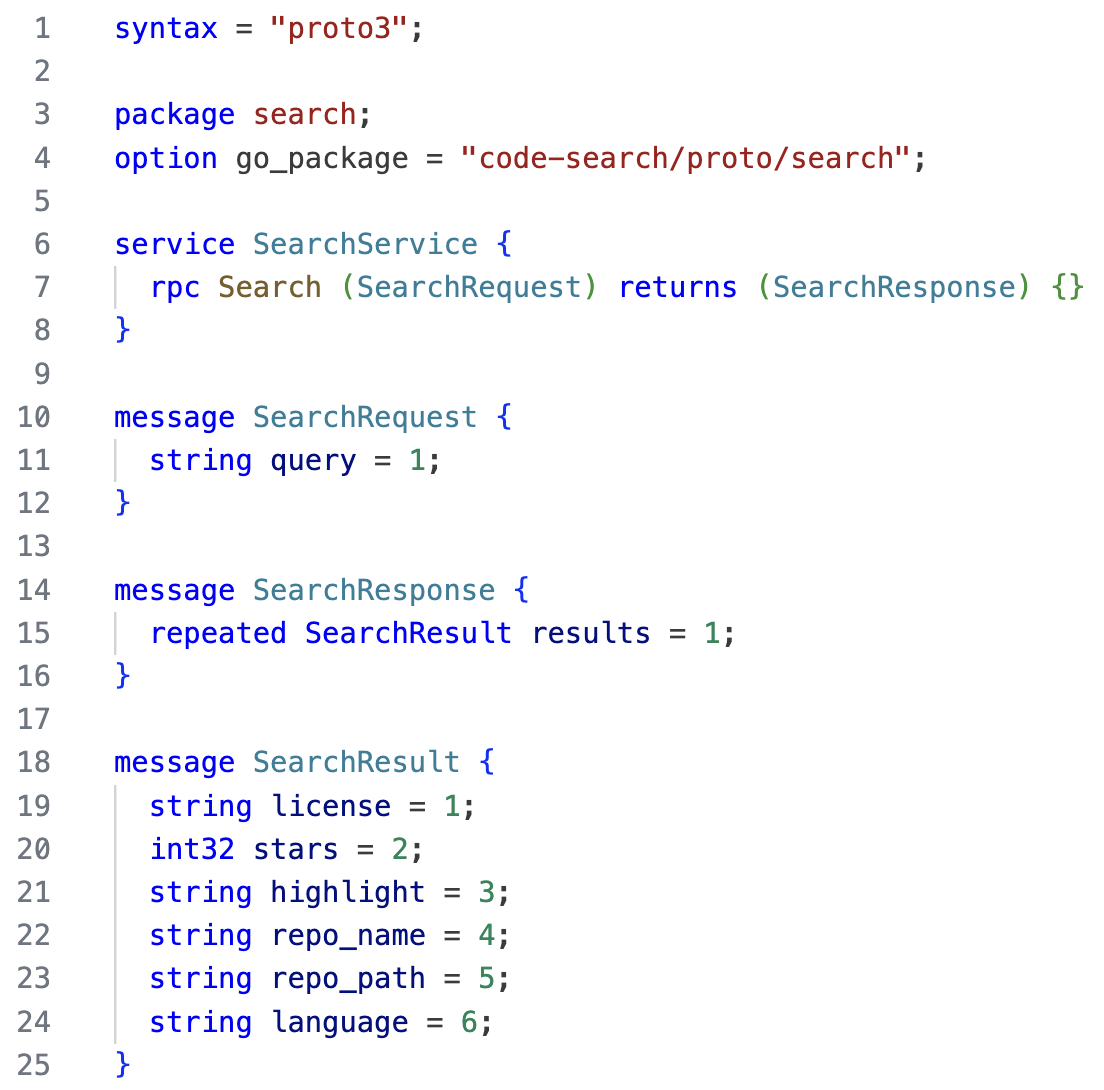
\includegraphics[width=0.95\textwidth]{search_proto.png}}
	\caption{智能搜索服务协议}
	\label{search_proto}
\end{figure}
用户的检索请求通过Search接口提交,SearchRequest与SearchResponse分别定义了请求与响应的数据结构。其中,SearchResponse结构体包含SearchResult列表,用于承载多样化的检索结果,支持多语言、多协议和多维度的代码查询需求。系统整体的用户搜索流程如图\ref{timeline}所示,用户经过鉴权后提交检索请求,系统将用户的原始查询语句发送至模型侧。模型对用户查询意图进行深度理解与专业化改写,并将优化后的检索词返回给查询系统。系统再将经过大模型处理的检索请求发送至底层数据库,数据库返回查询结果,最终由系统进行可视化展示。\par
\begin{figure}[H]
	\center{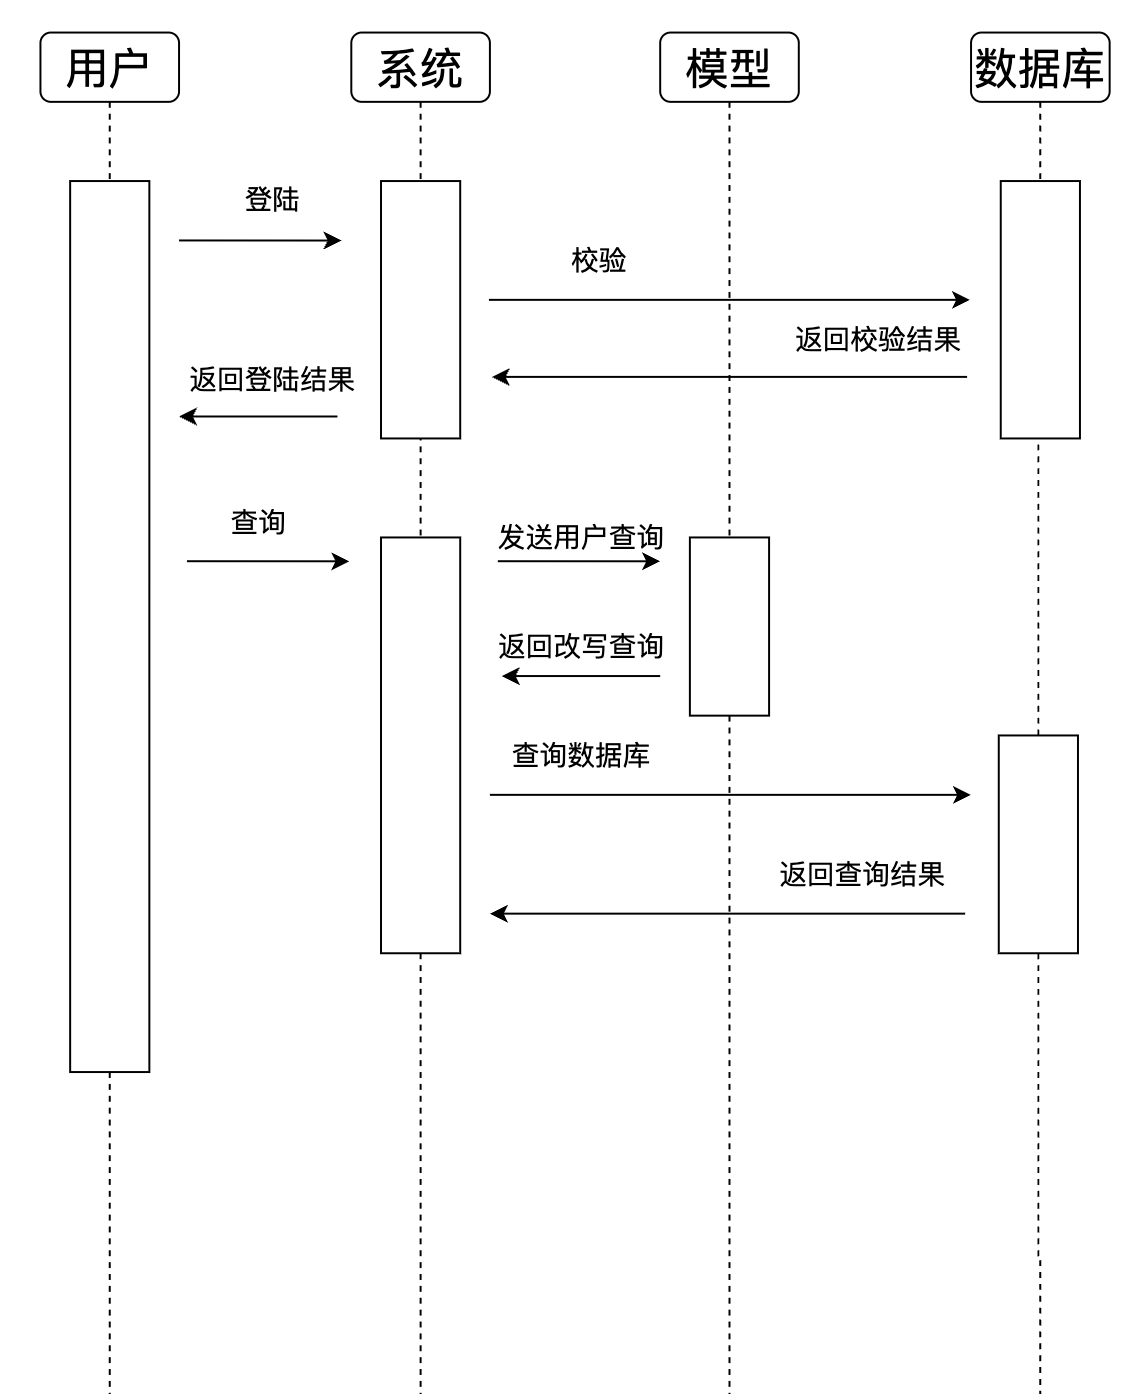
\includegraphics[width=0.95\textwidth]{timeline.png}}
	\caption{用户搜索时序图}
	\label{timeline}
\end{figure}
Elasticsearch作为底层分布式检索引擎,承担着代码数据的高效存储、索引与查询任务。为满足多语言、多协议、多维度的检索需求,系统在Elasticsearch中为代码数据设计了结构化的Mapping,如表\ref{esmapping}所示。
\begin{table}[H]
	\centering
	\caption{索引code的映射结构}
	\label{tab:code_mapping}
	\small
	\begin{tabular}{c c c}
		\toprule
		字段名 & 数据类型 & 描述 \\
		\midrule
		content & text & 代码内容(文本类型) \\
		file\_name & keyword & 文件名(关键字类型) \\
		repo\_name & keyword & 文件所属项目名(关键字类型)\\
		lang & keyword & 编程语言(关键字类型) \\
		lic & keyword & 许可证类型(关键字类型) \\
		stars & integer & 星标数量(整数类型) \\
		\bottomrule
	\end{tabular}
	\label{esmapping}
\end{table}
在该Mapping结构中,content字段采用text类型,支持分词和全文检索,能够对代码内容进行高效的语义匹配和相关性排序。file\_name和repo\_name字段采用keyword类型,便于对特定文件或项目进行精确过滤和聚合统计,同时也方便在搜索结果中展示文件和项目的详细信息。lang字段用于标识代码所使用的编程语言,lic字段记录代码的开源协议类型,这两个字段均为keyword类型,能够支持高效的条件过滤和多维度聚合分析。stars字段则记录项目的星标数量,采用integer类型,便于对检索结果进行数值排序和统计分析,例如优先展示高星项目或实现项目热度排行。基于上述Mapping结构,系统能够灵活支持多维度的检索需求。在实际查询流程中,服务端会根据LLM生成的结构化检索指令,将用户的查询意图映射到Elasticsearch的复合查询语句中,从而提升查询的联想能力以及准确性。
\subsection{基于提示词工程的查询上下文增强技术}
为实现查询语句的山下文增强功能,本文设计了一种多层次的提示词模板,其基本结构如图\ref{prompt1}所示。该结构以“任务-思维链-结构化输出”为核心,系统性地分解和重构用户的自然语言查询。具体而言,提示词首先引导大语言模型依次分析语言、协议、技术三个维度,既能够捕捉用户的显性需求,也能挖掘隐含的上下文信息和技术细节。模型需判断查询是否针对特定编程语言,并据此设定检索范围;其次,识别用户对开源协议的潜在要求,确保检索结果的合规性;最后,深入分析与查询相关的API、库、框架及典型技术关键词,提升检索的专业性和覆盖面。在输出格式上,提示词模板采用<Think>标签对模型的推理过程进行显式分层,要求模型分别阐述对每一维度的分析思路,增强推理的可解释性和透明度。最终,系统将分析结果以结构化的JSON格式输出,明确标注检索语言、协议要求及技术关键词,为后续的代码检索模块提供高质量、可直接执行的查询指令。\par
\begin{figure}[H]
	\center{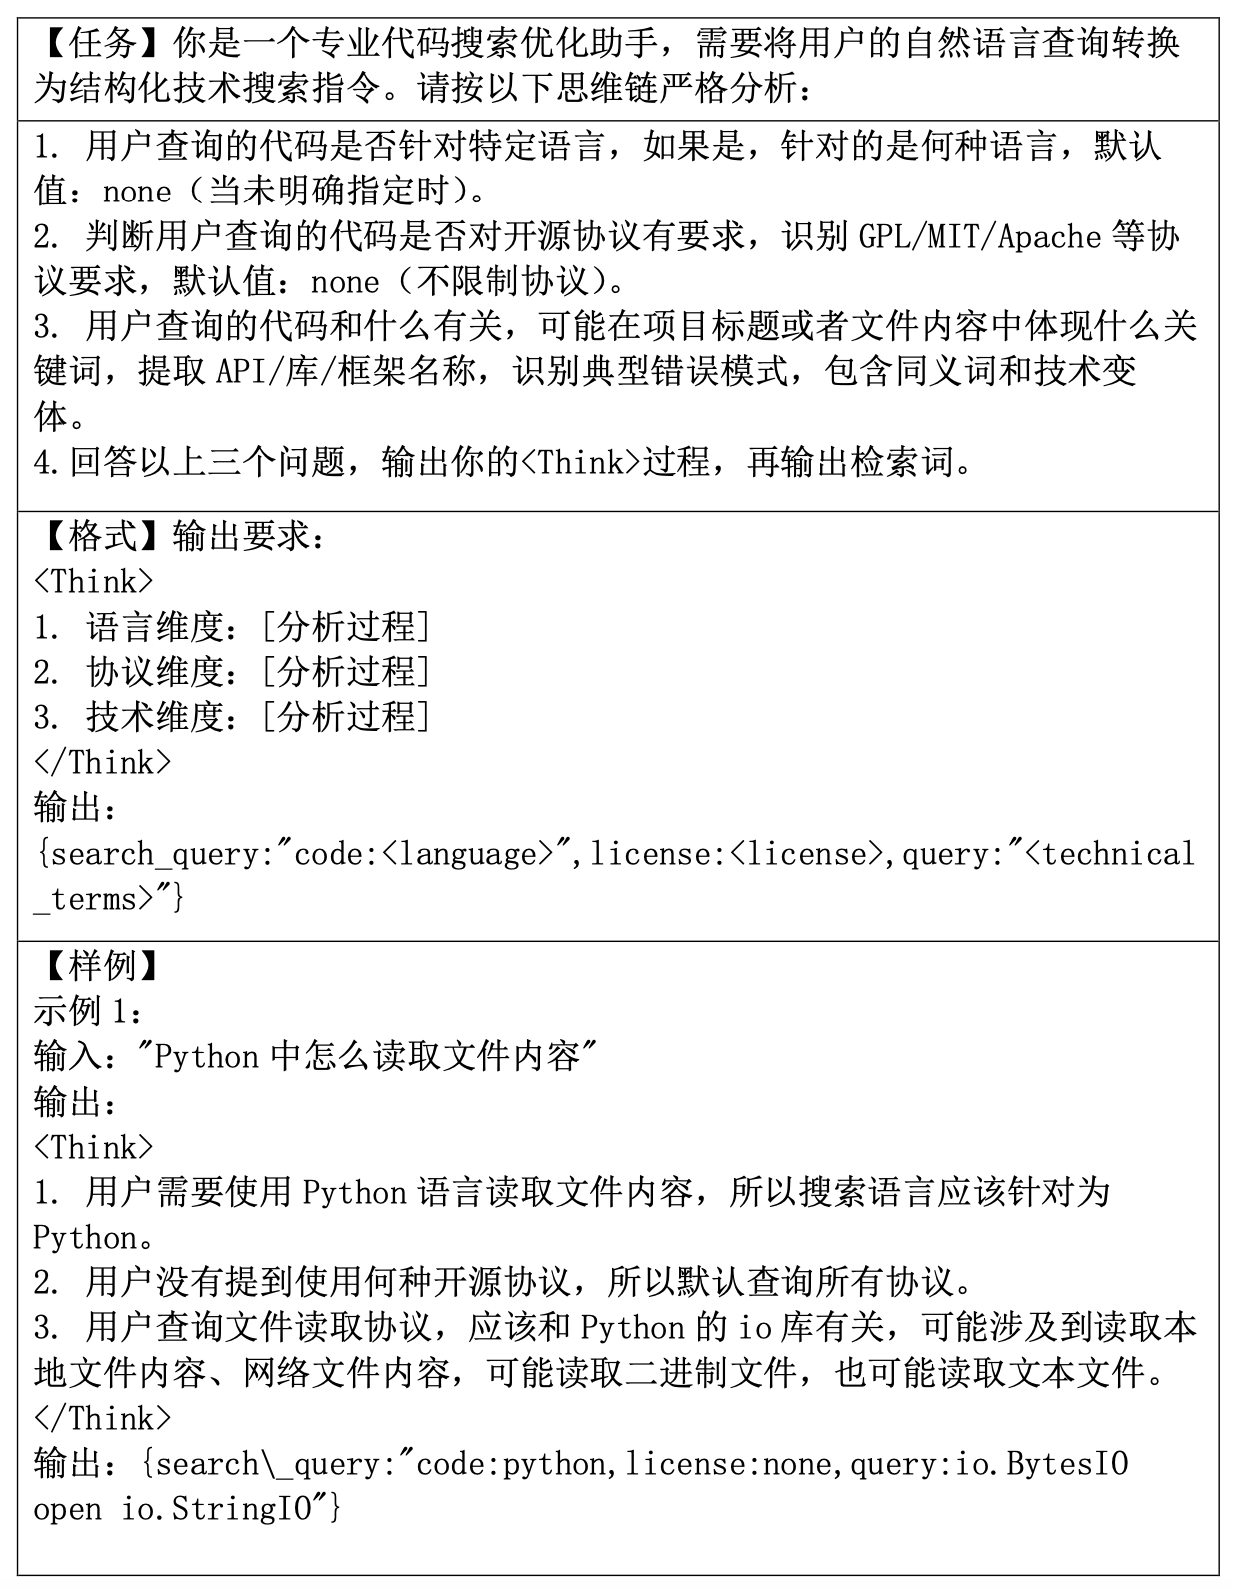
\includegraphics[width=0.95\textwidth]  {prompt1.png}} 
	\caption{提示词结构}
	\label{prompt1}
\end{figure}
\begin{figure}[H]
	\center{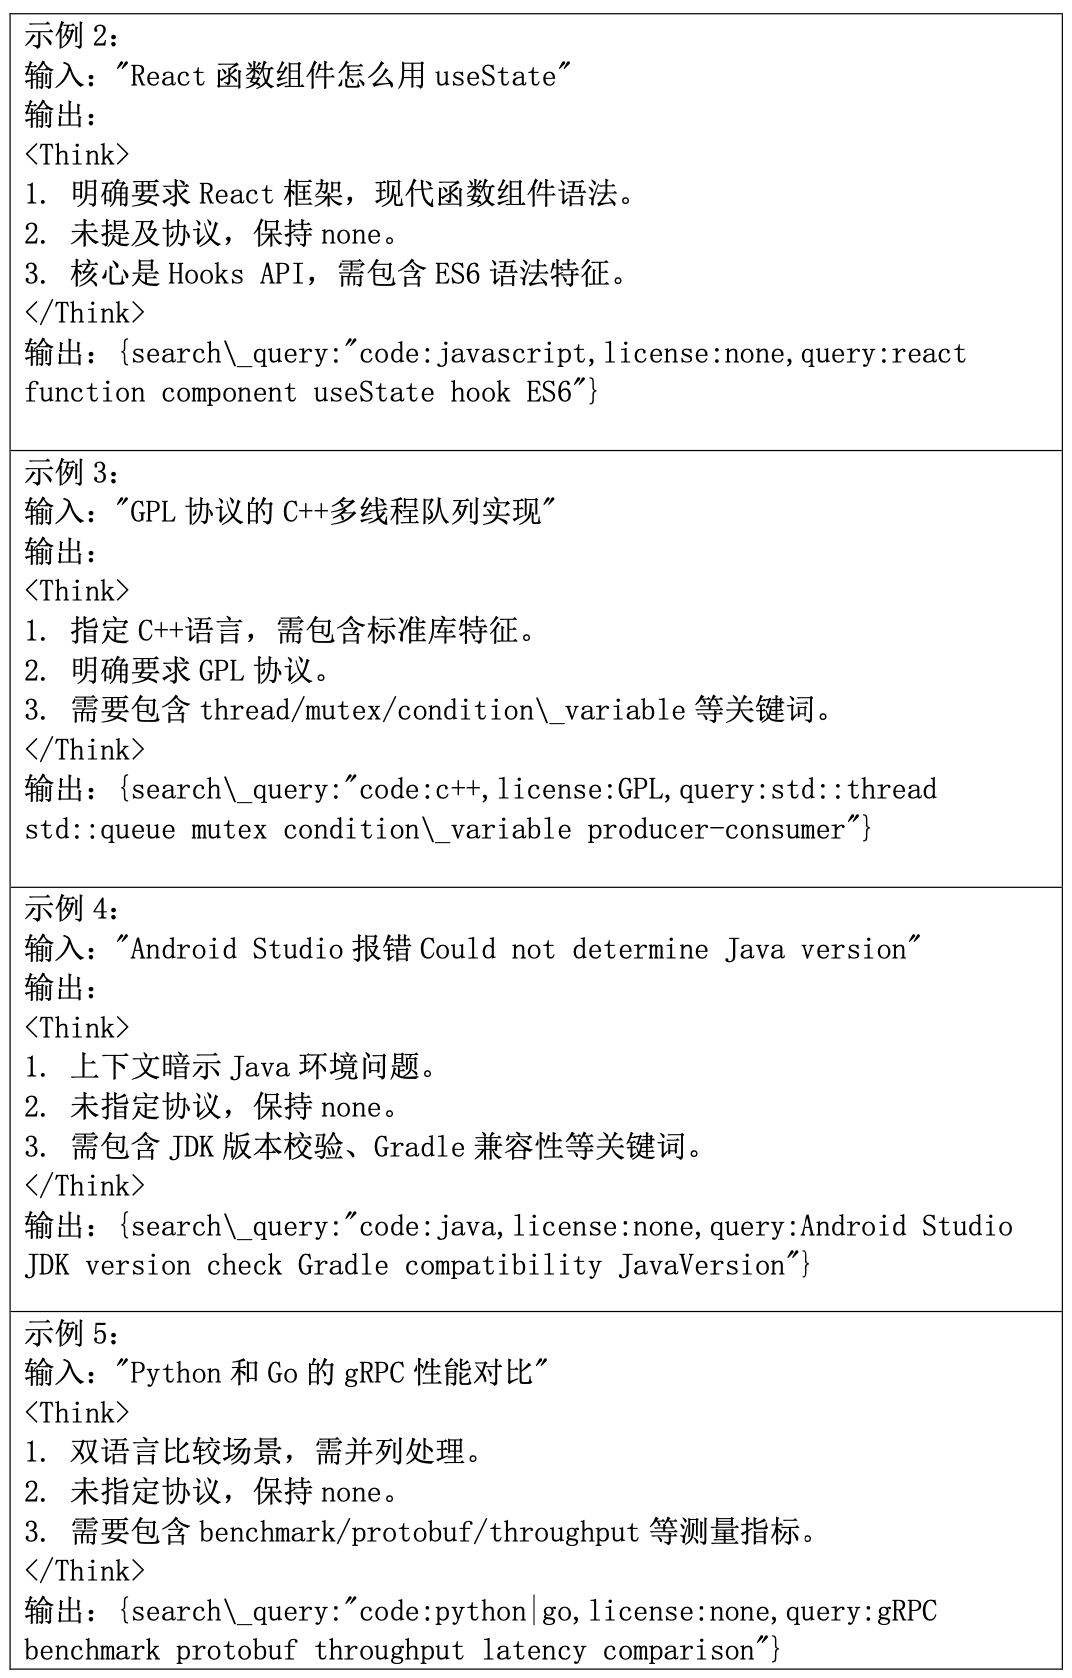
\includegraphics[width=0.95\textwidth]  {prompt2.png}} 
	\caption{提示词结构}
	\label{prompt2}
\end{figure}
进一步地,如图\ref{prompt2}所示,本文引入了few-shot示例驱动的提示词工程方法。通过在提示词模板中配备多样化的输入输出示例,涵盖单语言检索、框架API查询、协议限定、错误诊断及多语言对比等典型场景,模型能够更好地学习如何将复杂、模糊的自然语言需求转化为精确、结构化的检索表达。few-shot示例不仅为模型提供了明确的任务范式和推理参考,还显著提升了模型在多编程语言代码检索任务中的理解能力和检索准确率。通过这种“任务-思维链-结构化输出”的提示词工程方法,系统能够有效适应多样化的用户需求,提升整体检索性能和用户体验。
\subsection{智能代码检索系统前端界面设计实现}
系统支持通过VS Code插件进行代码检索,极大提升了用户的使用便捷性。插件依托VS Code提供的 \texttt{vscode.WebviewViewProvider} 接口开发,将前端Web页面无缝集成到VS Code左侧Tab栏。用户只需点击Tab栏按钮,即可进入代码搜索界面,体验与Web端一致的检索与结果展示功能。插件界面如图\ref{vscode}所示。插件内部采用与Web端相同的Vue组件和状态管理方案,确保功能和交互体验的一致性。同时,插件通过VS Code的消息传递机制实现与扩展后台的通信,支持异步请求和结果回传,保证检索过程的流畅与稳定。
\begin{figure}[H]
	\center{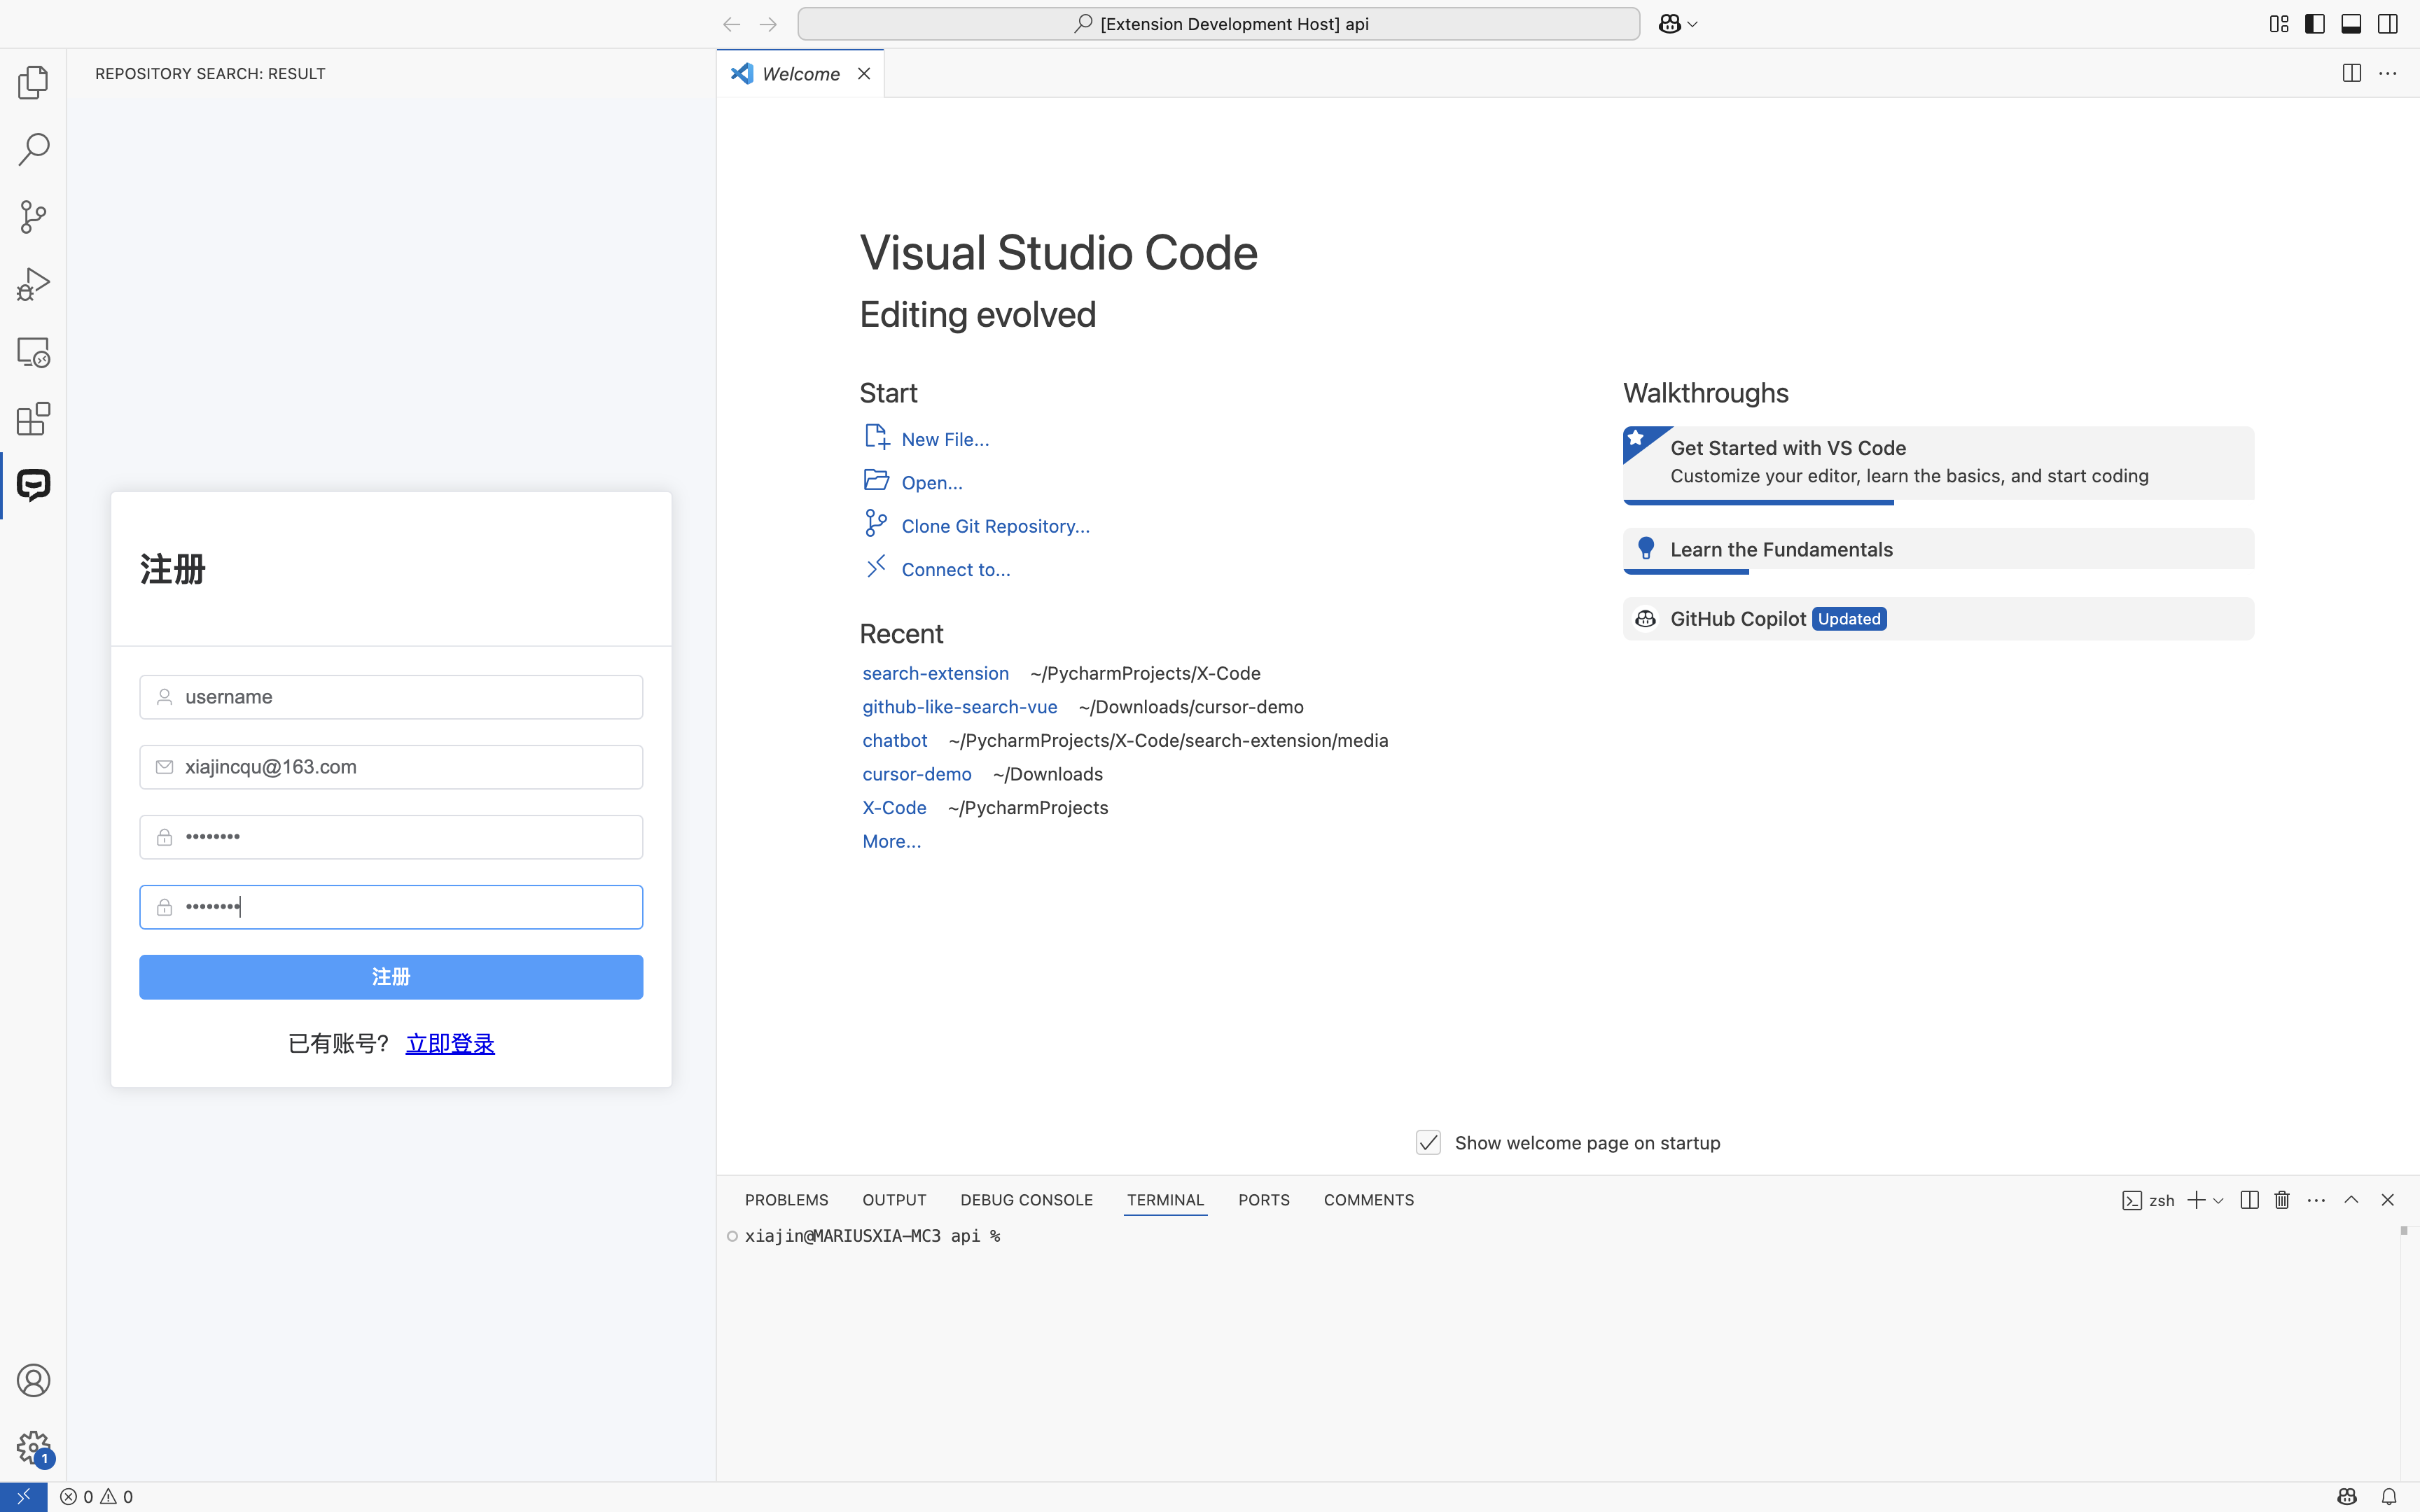
\includegraphics[width=0.95\textwidth]{register.png}}
	\caption{VS Code插件页面}
	\label{vscode}
\end{figure}
在登录界面,如图\ref{logincheck}和图\ref{loginpage}所示,系统实现了账号密码输入的前端校验,防止空表单提交,提升系统安全性和用户体验。输入框绑定了实时校验规则,用户输入时即时反馈格式错误或缺失信息。用户信息在前端通过加密算法进行加密处理后,安全传输至后端进行身份校验,保障数据传输安全。登录失败时,界面会给出明确的错误提示,帮助用户快速定位问题。
\begin{figure}[H]
	\center{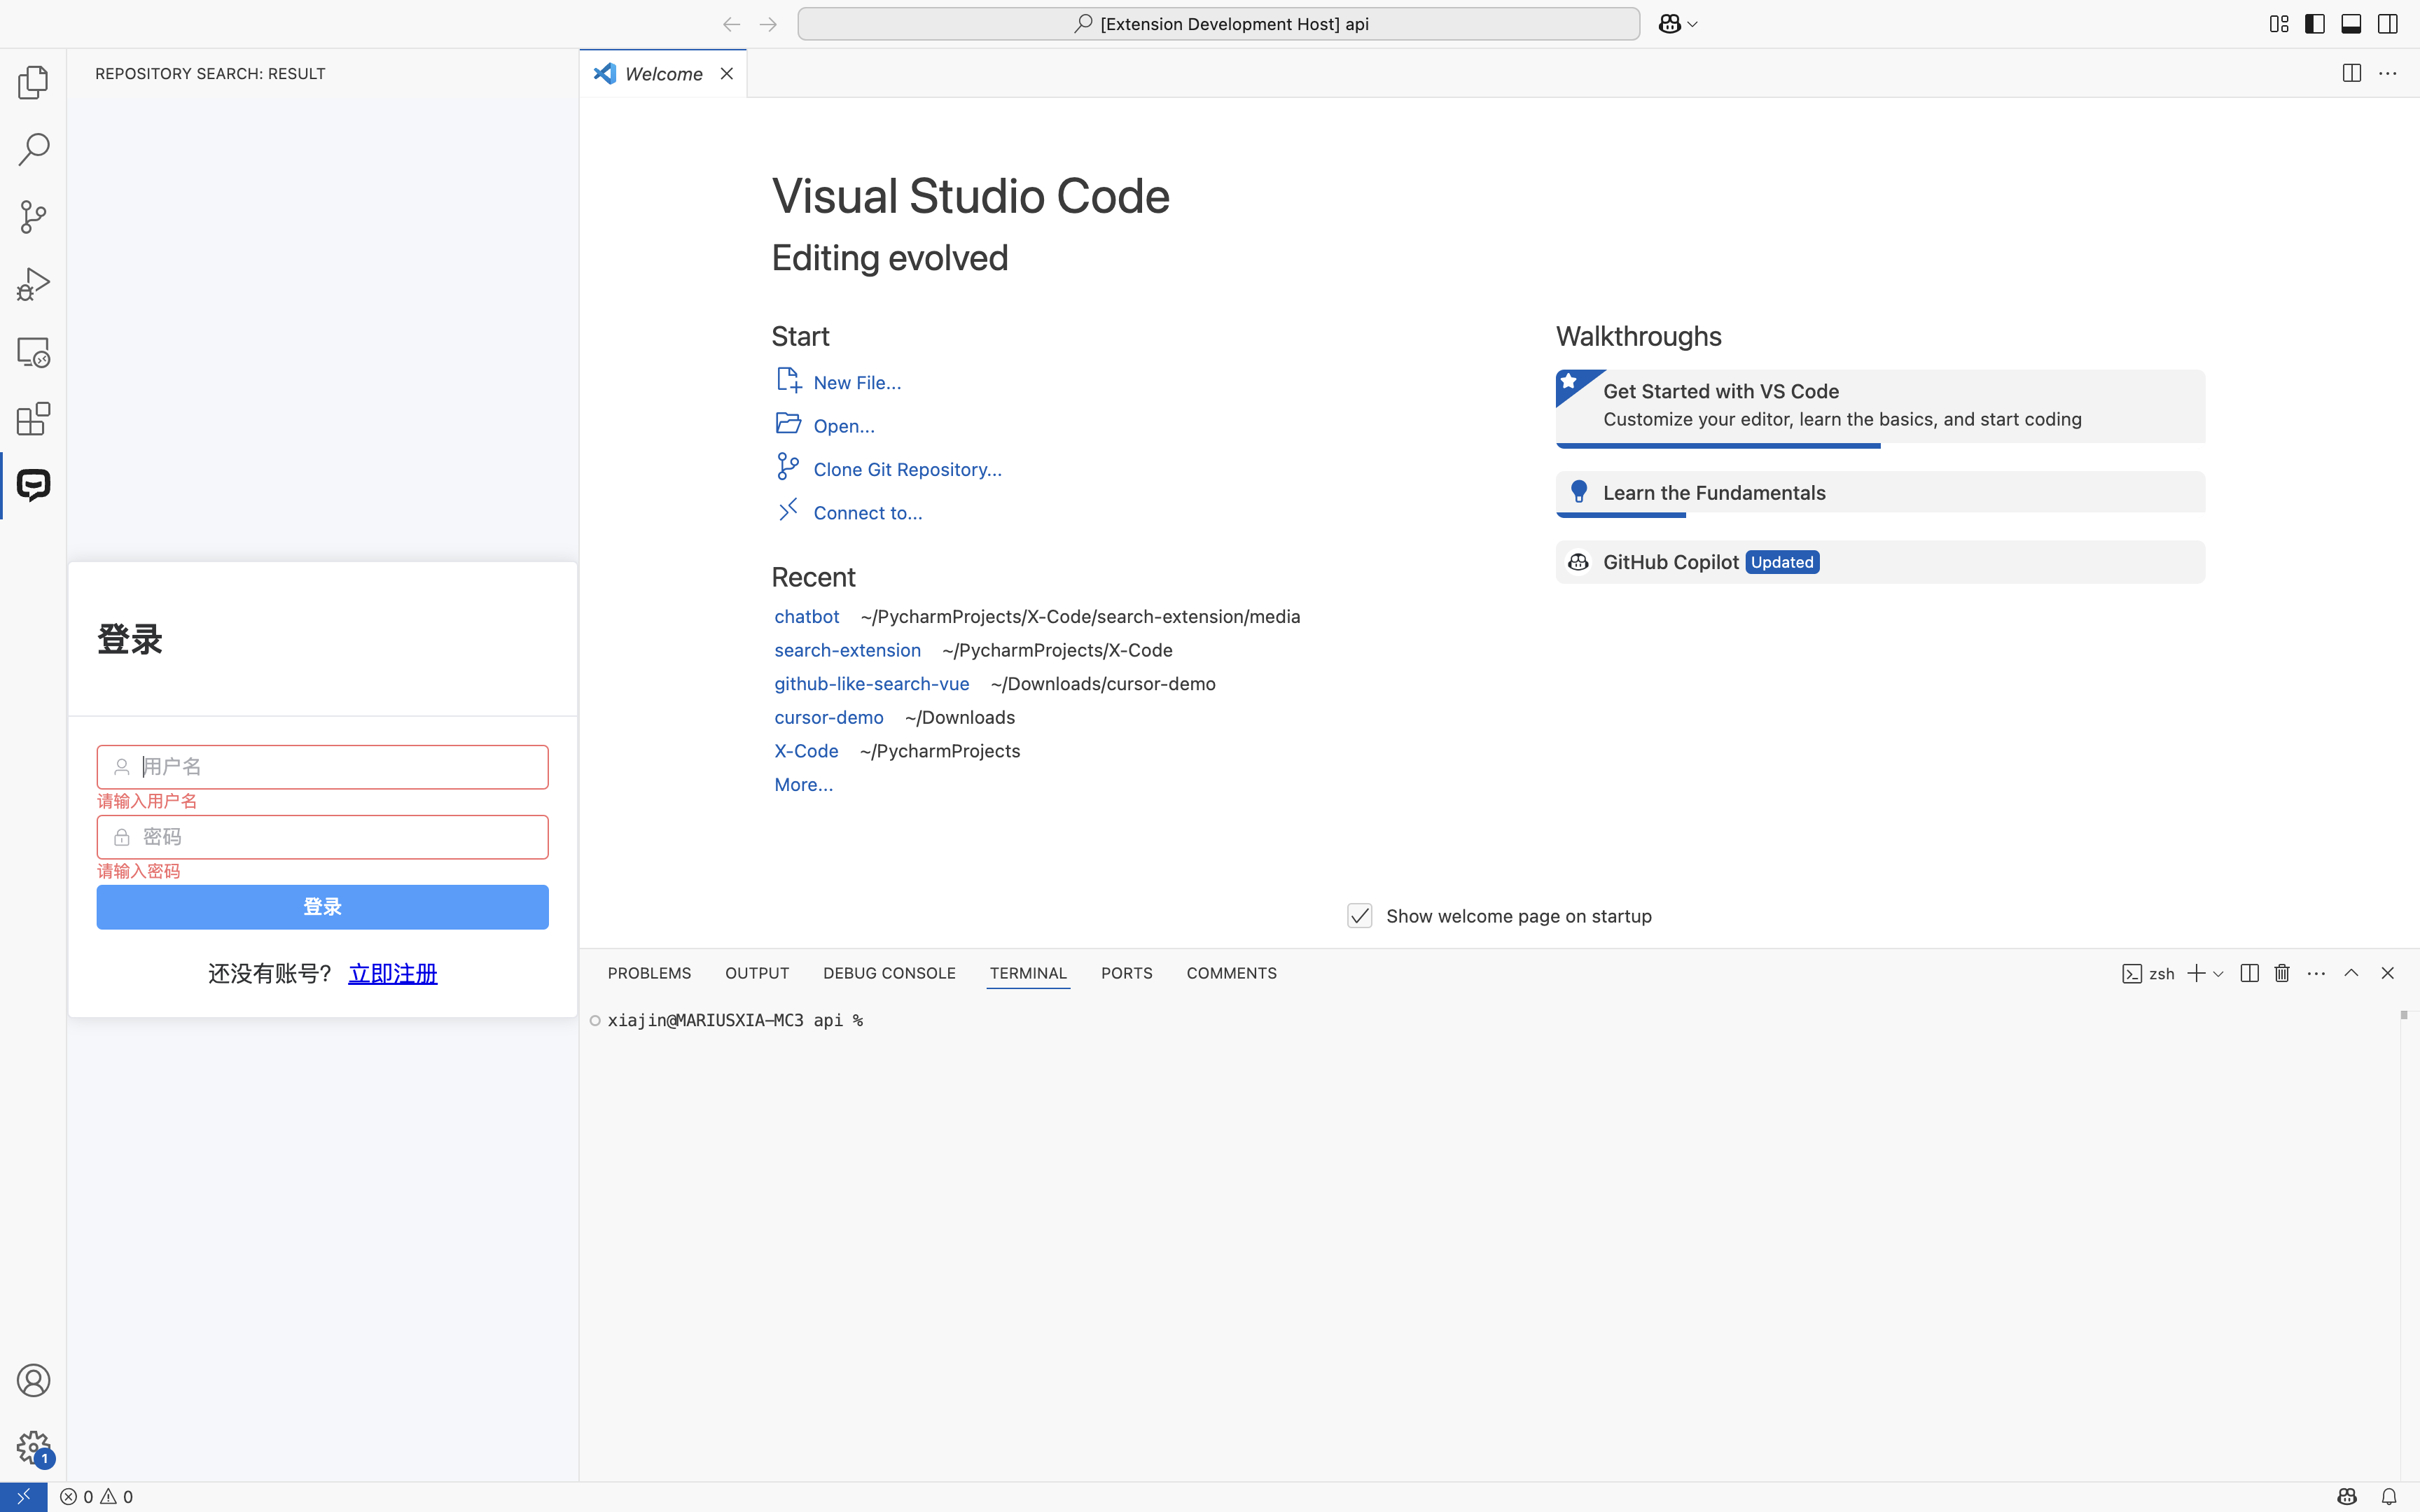
\includegraphics[width=0.95\textwidth]{login_check.png}}
	\caption{登录校验示例}
	\label{logincheck}
\end{figure}
\begin{figure}[H]
	\center{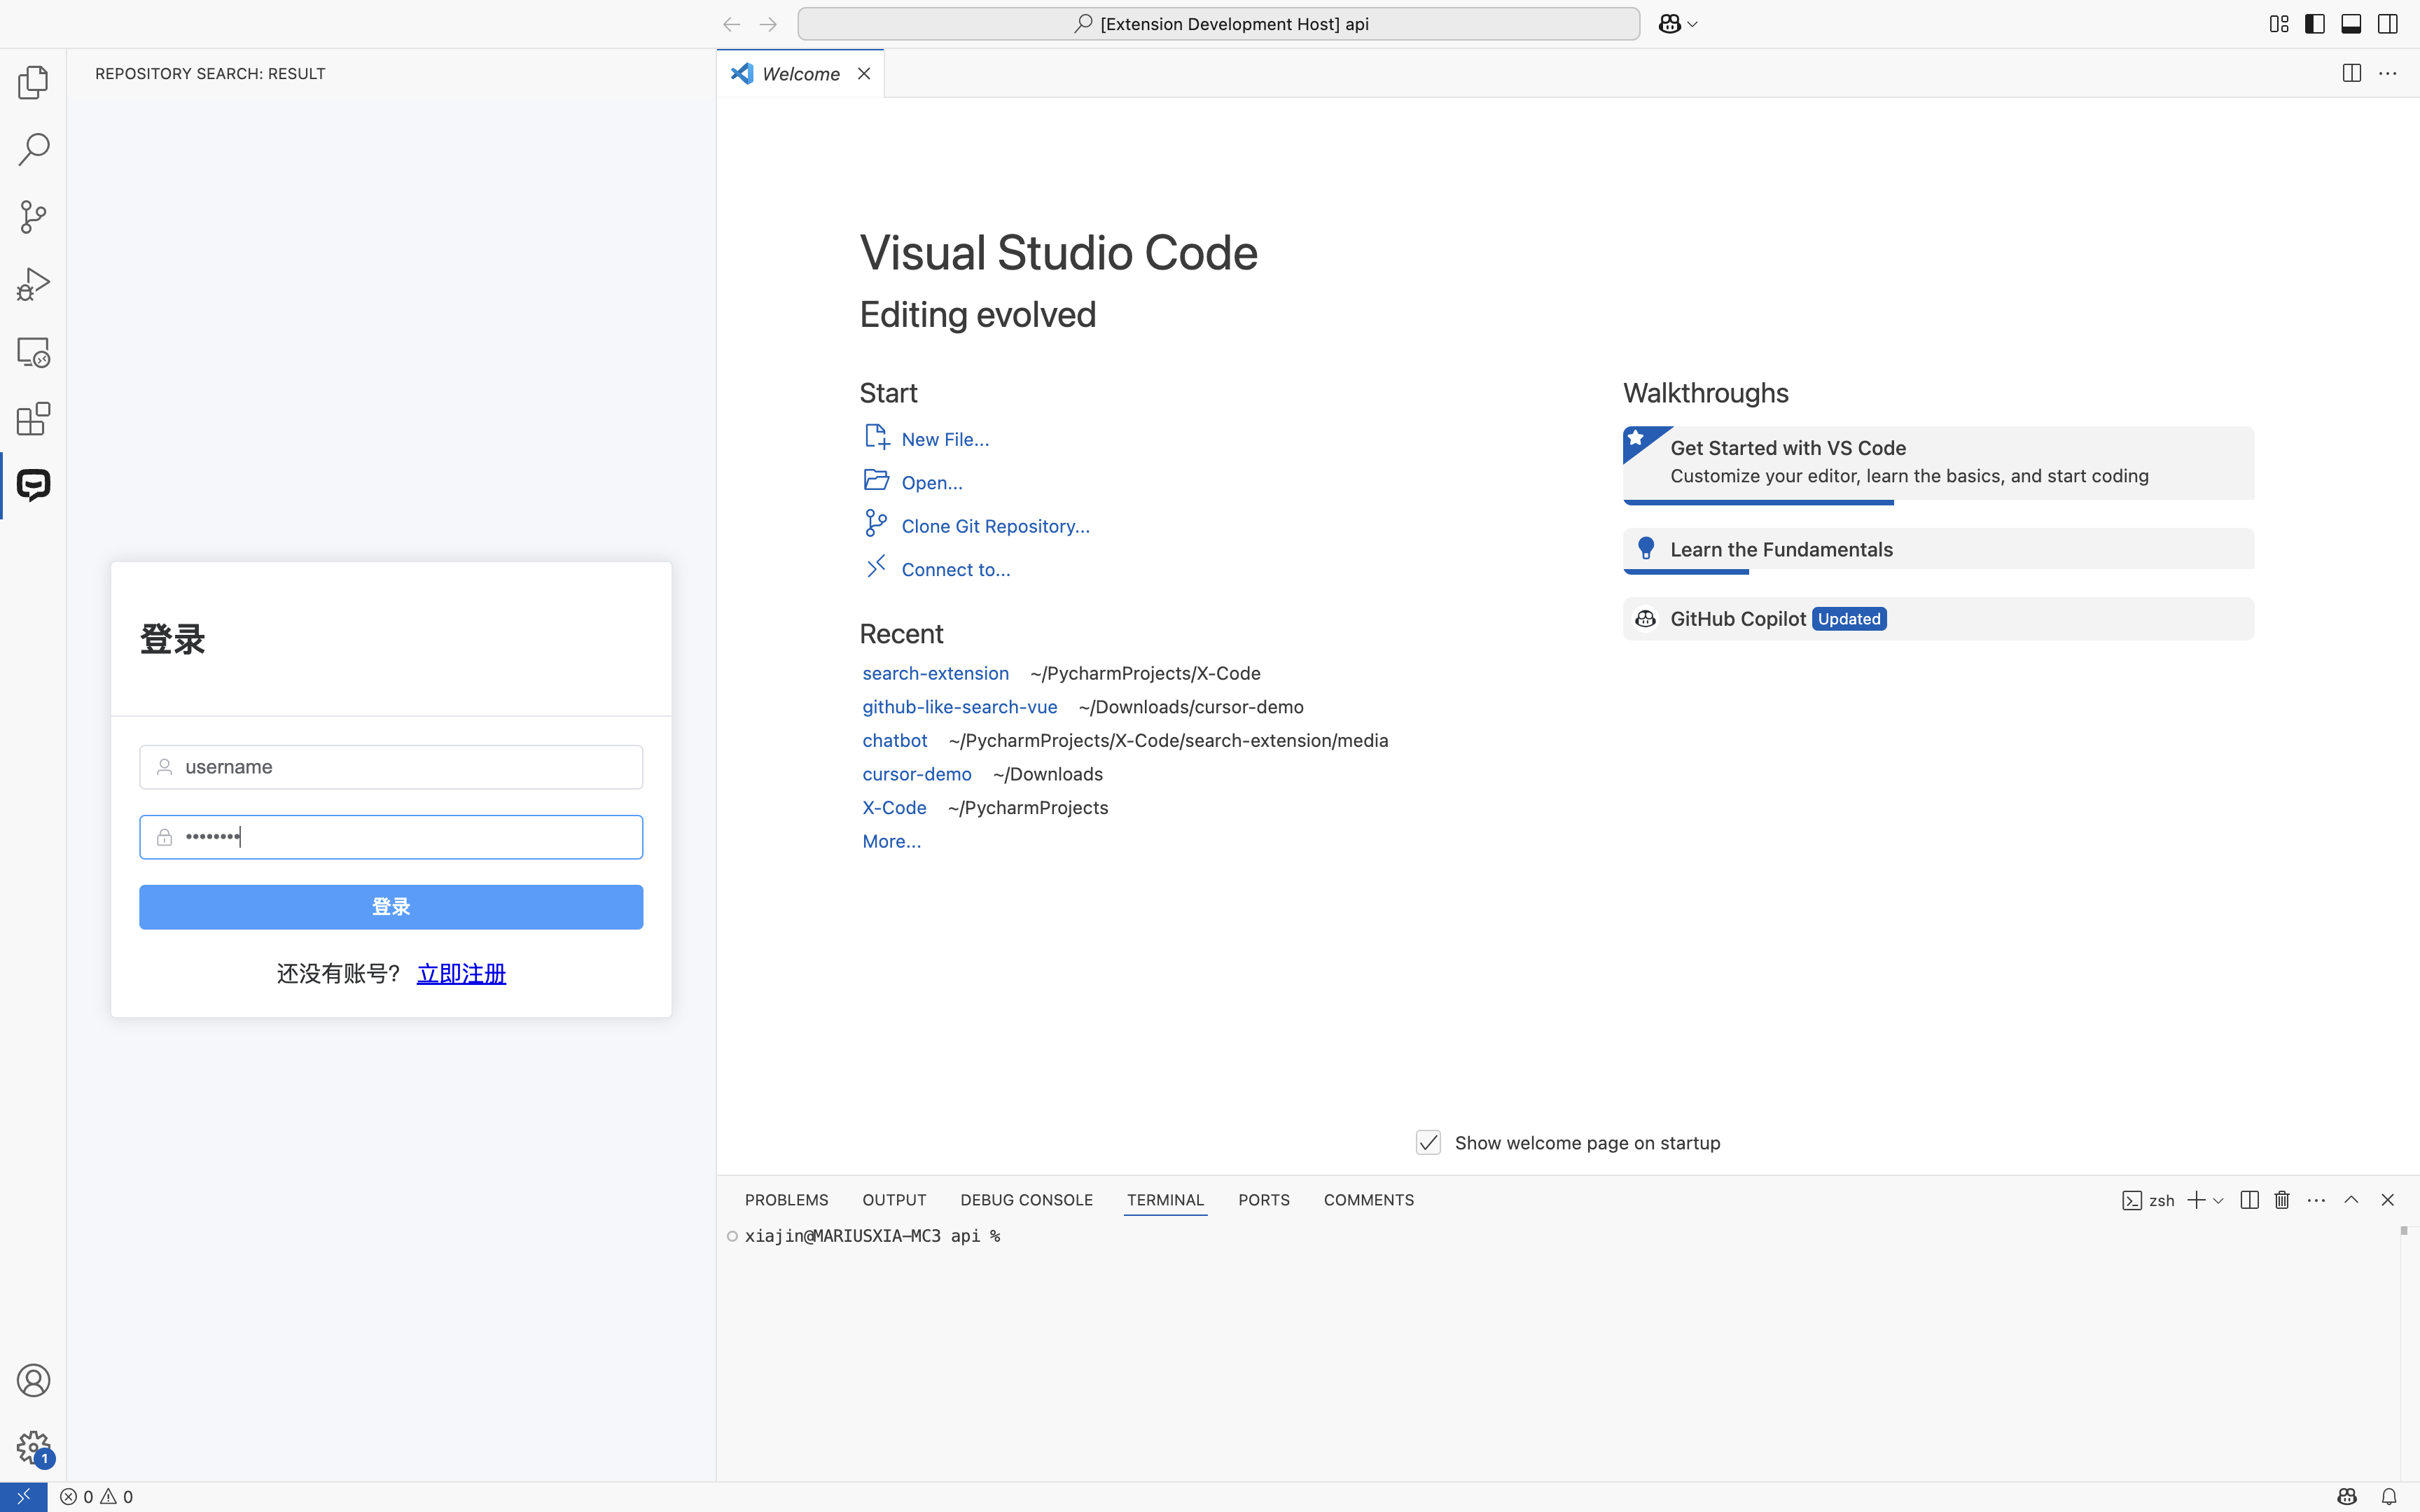
\includegraphics[width=0.95\textwidth]{login.png}}
	\caption{登录示例}
	\label{loginpage}
\end{figure}
注册页面同样具备完善的输入检测功能,支持密码一致性校验、邮箱格式验证及用户名合法性检查,防止无效或恶意数据提交。如图\ref{registerpage}和图\ref{registercheckpage}所示,系统通过双向数据绑定实现表单状态的实时更新,用户填写信息时即刻获得有效性反馈。注册成功后,系统自动跳转至登录页面,提升用户操作的连贯性。
\begin{figure}[H]
	\center{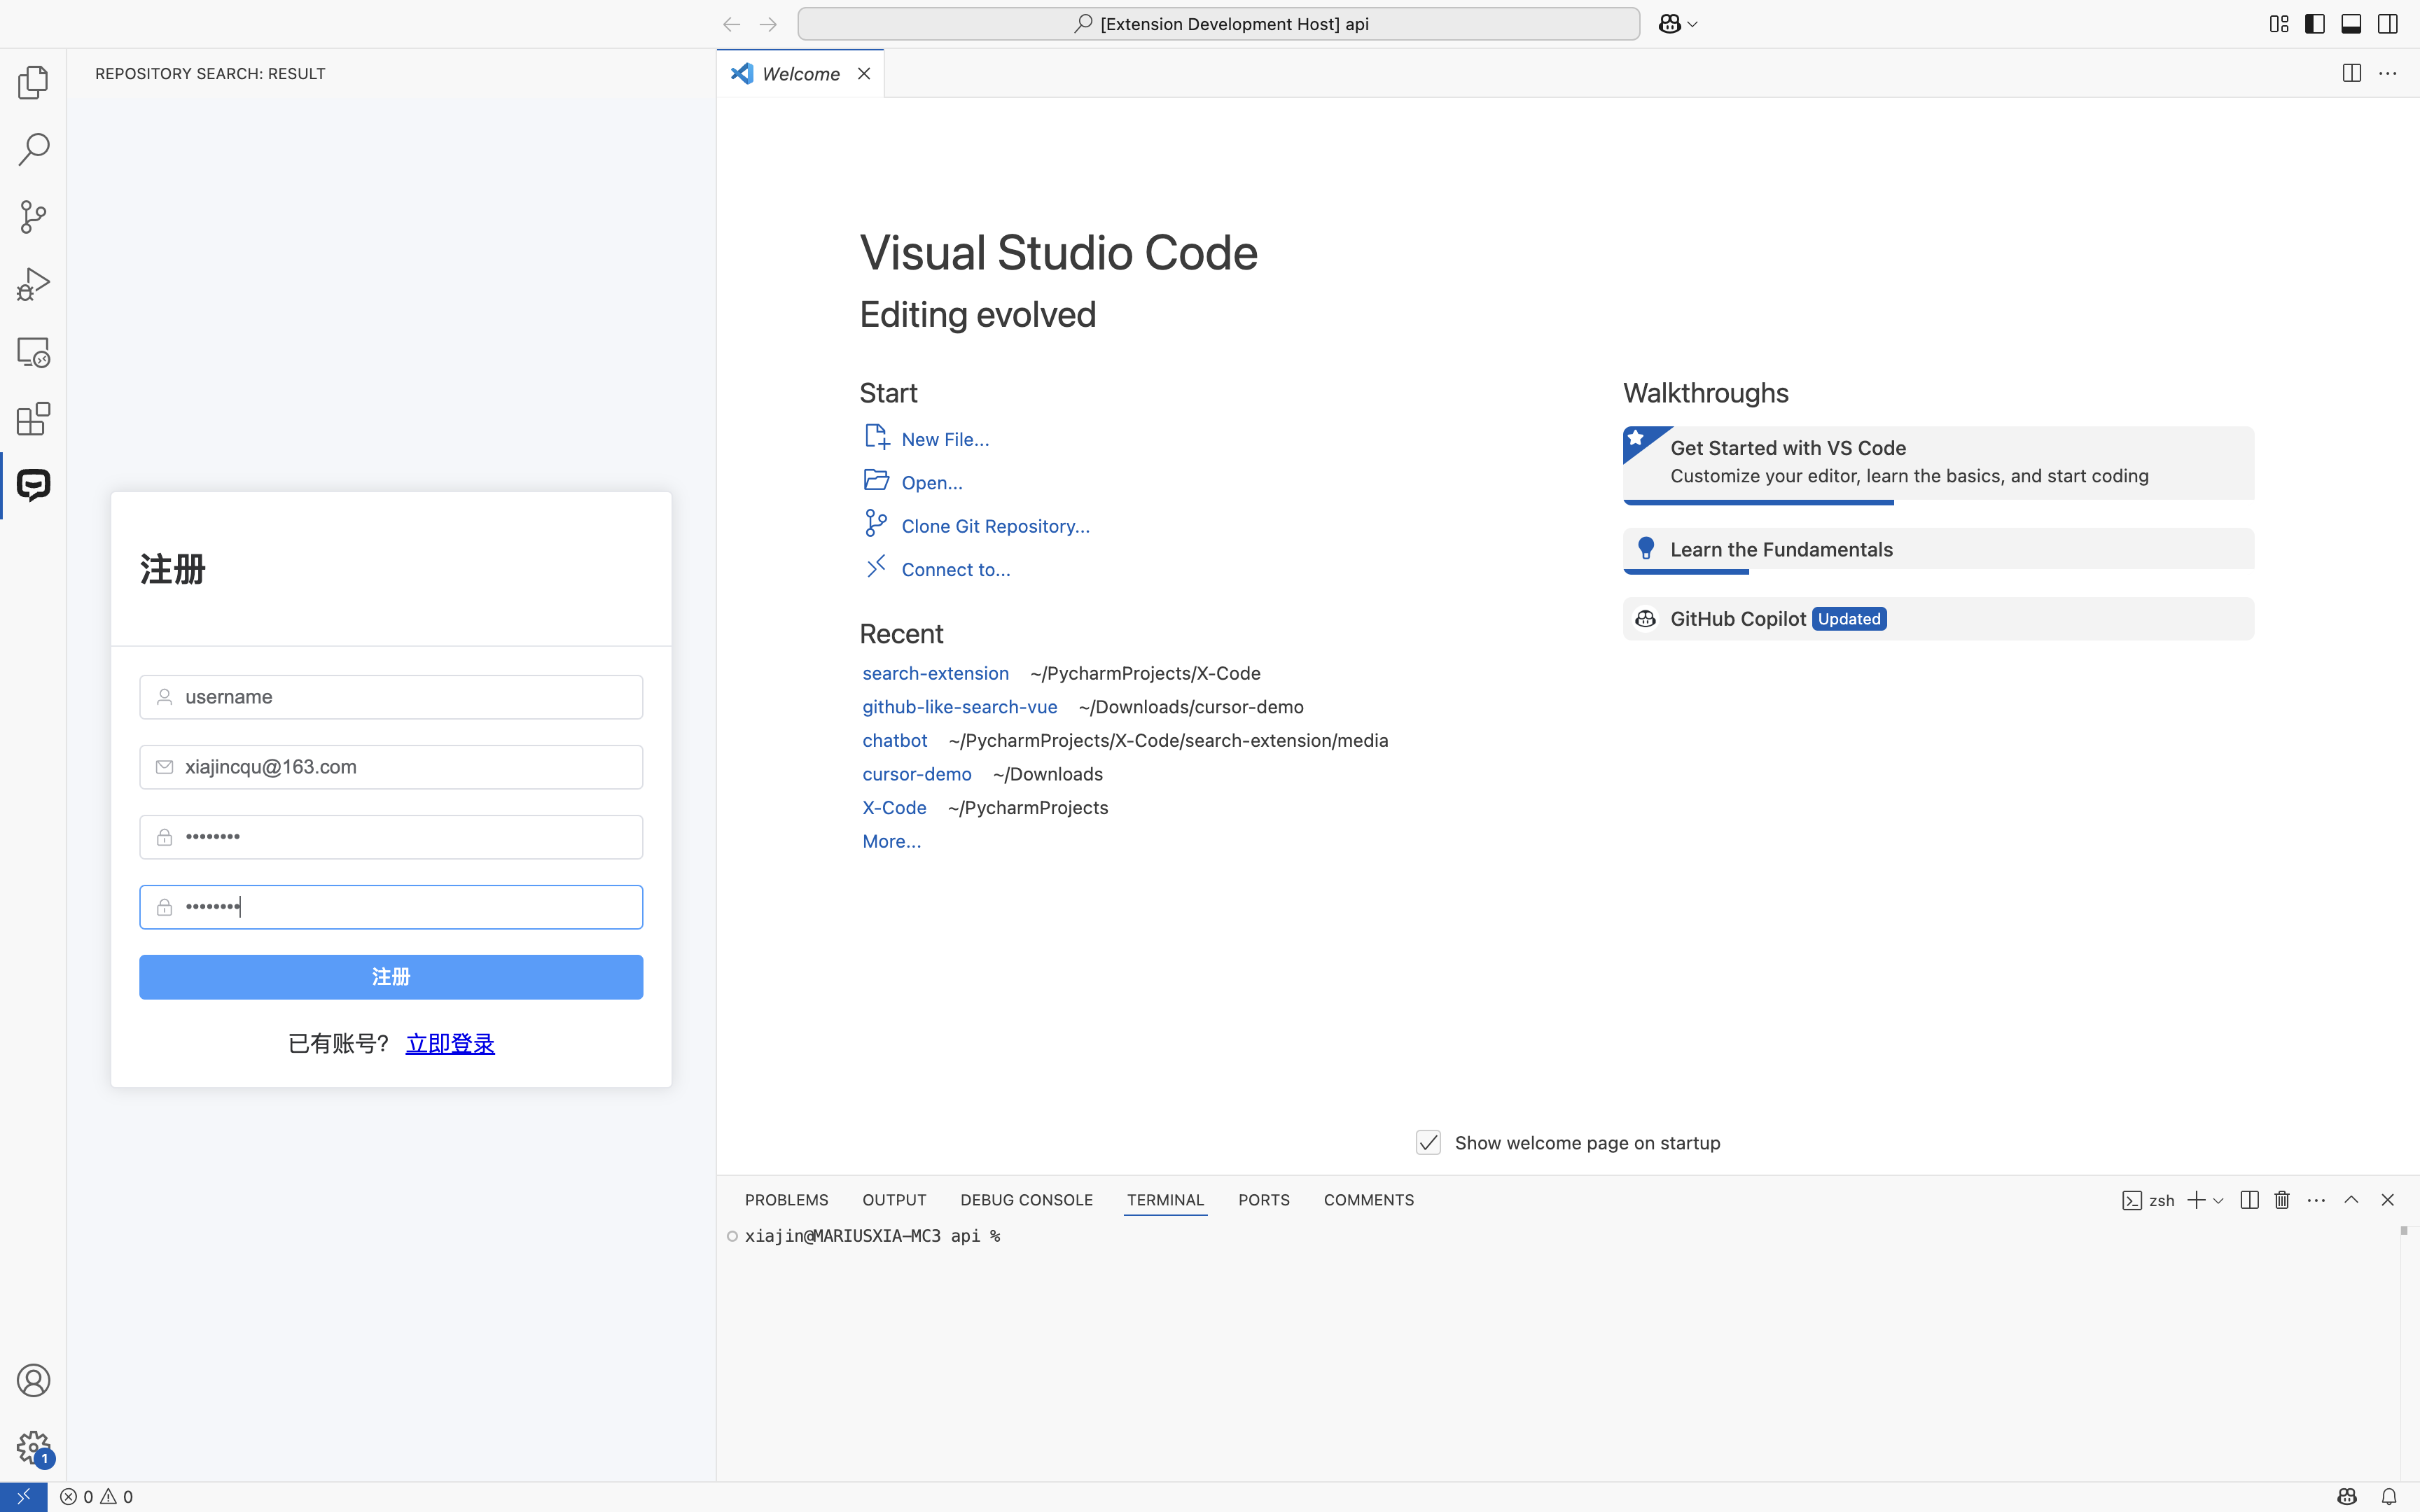
\includegraphics[width=0.95\textwidth]{register.png}}
	\caption{注册示例}
	\label{registerpage}
\end{figure}
\begin{figure}[H]
	\center{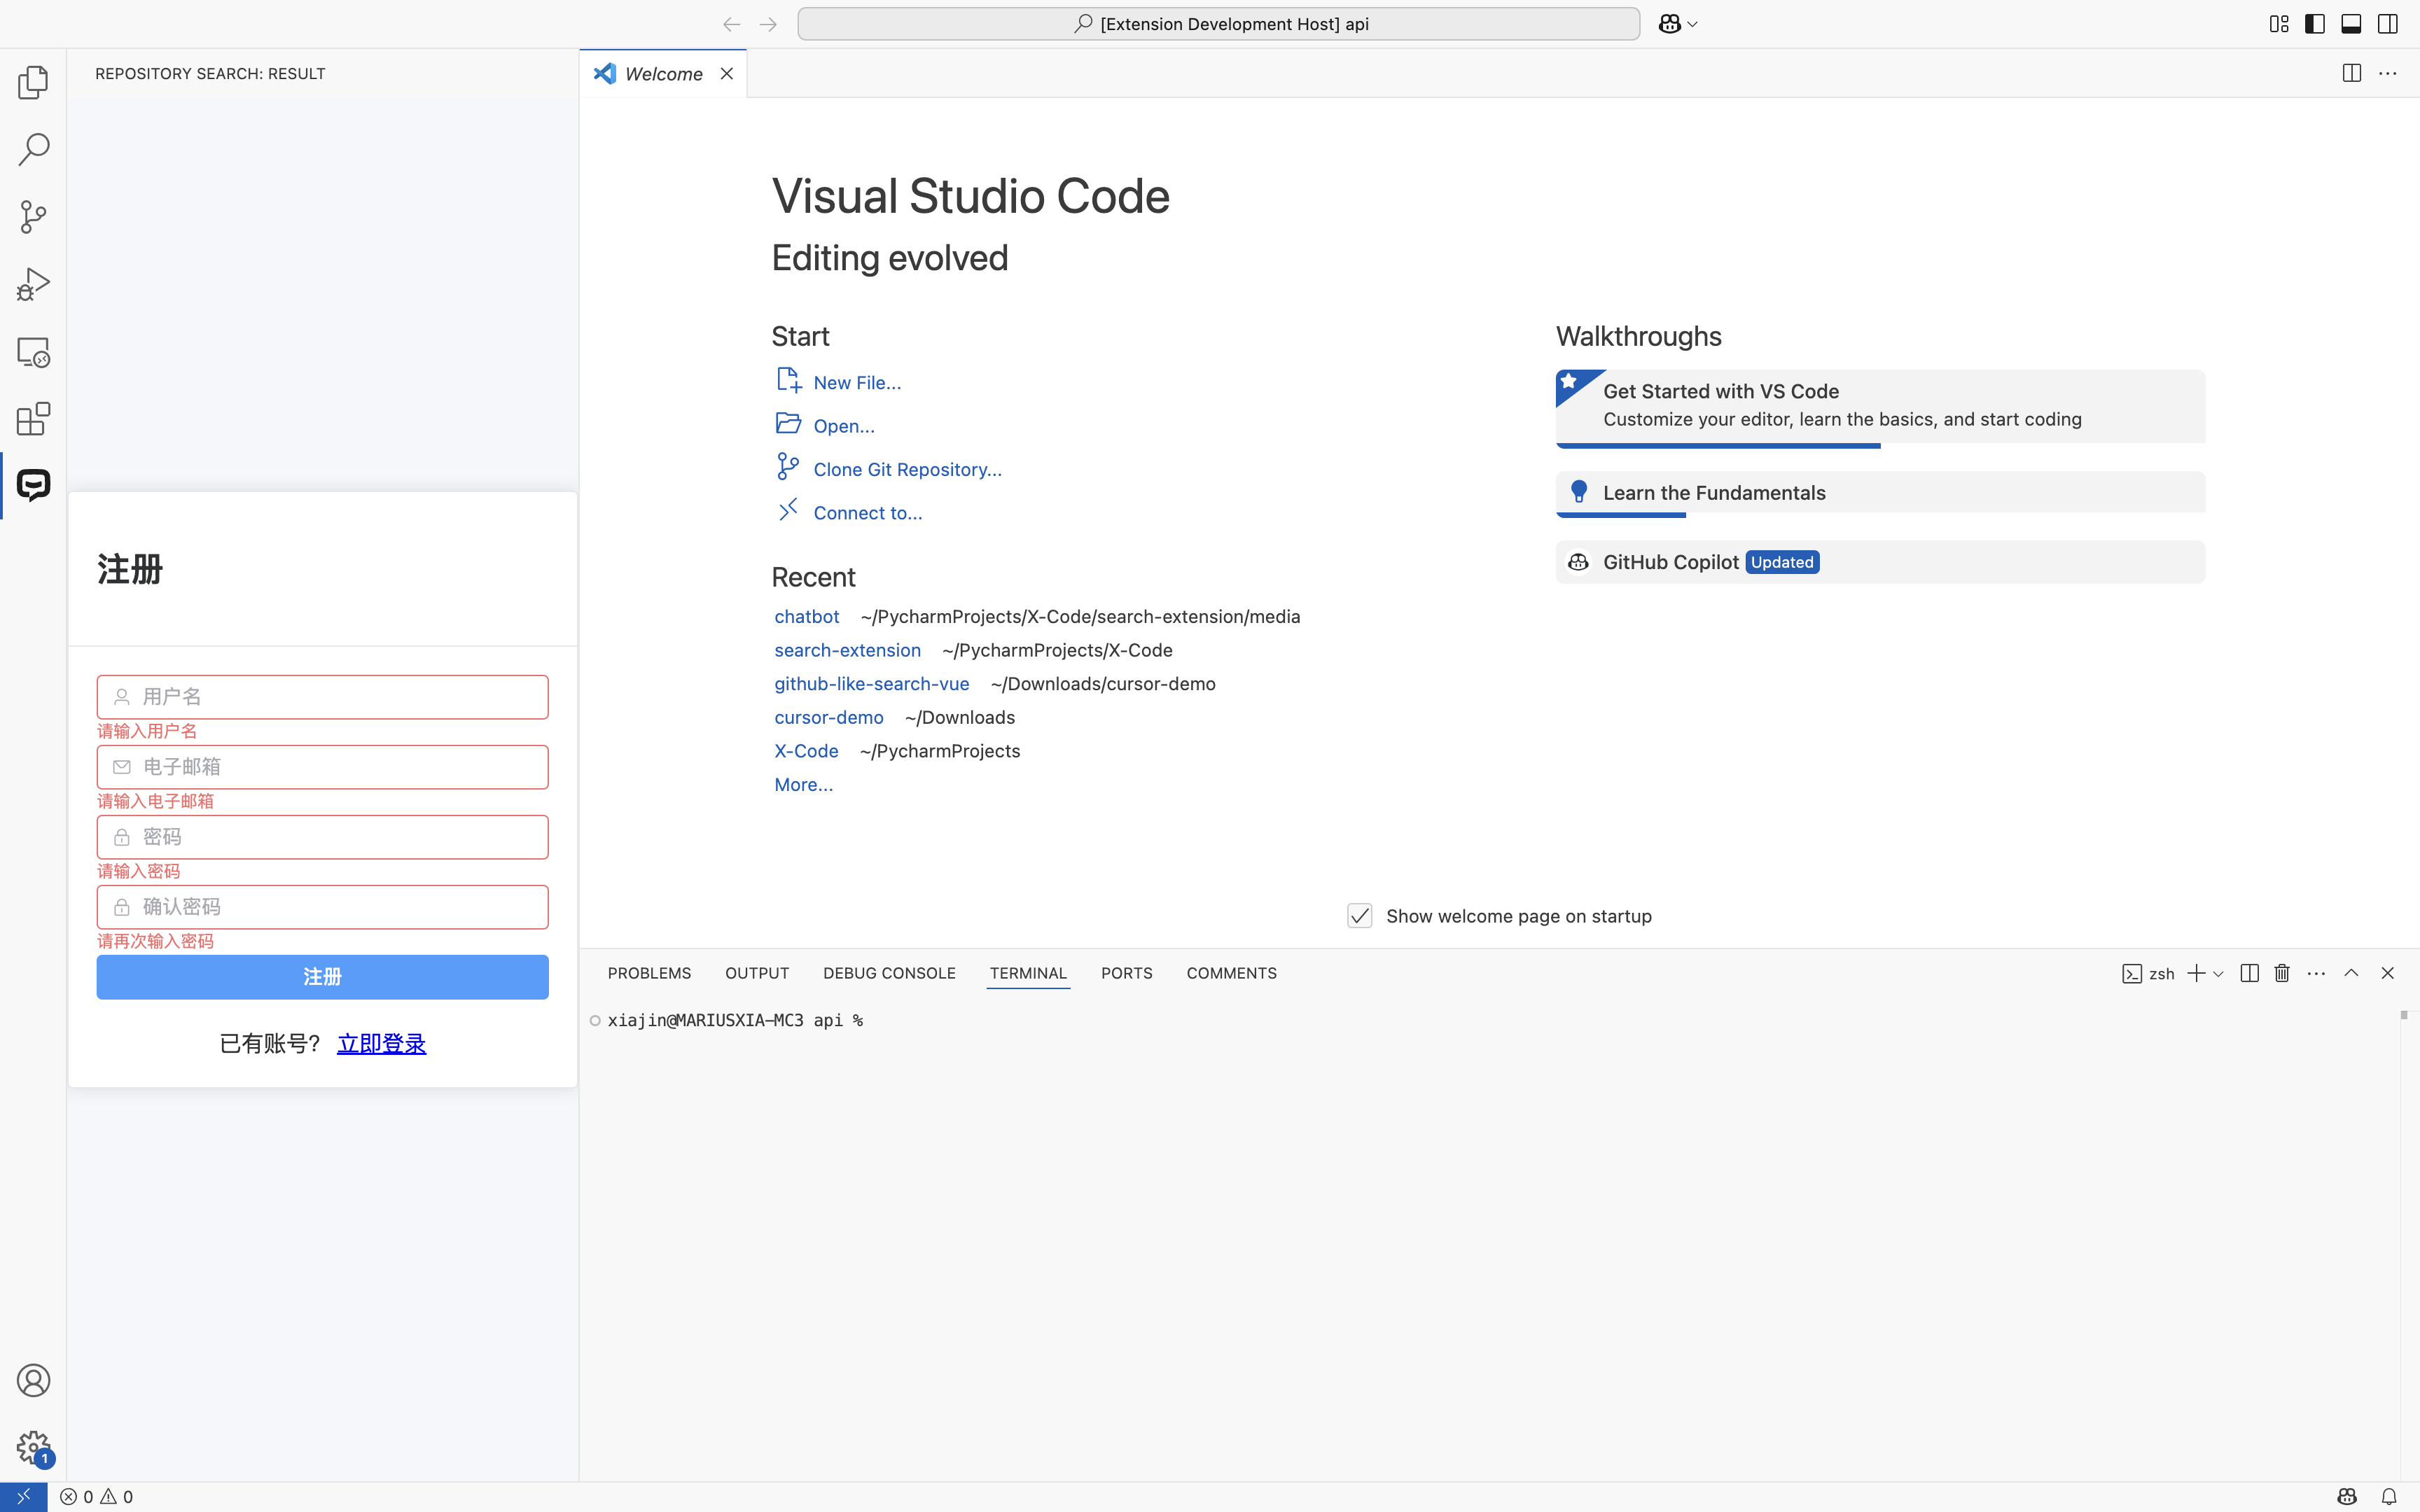
\includegraphics[width=0.95\textwidth]{register_check.png}}
	\caption{注册校验示例}
	\label{registercheckpage}
\end{figure}

系统的搜索页面设计简洁直观,用户可在输入框中输入关键词进行代码检索。与传统搜索引擎不同,系统在前端对用户输入的查询词进行智能改写和预处理(如同义词扩展、语义纠正等),并通过后端专业查询方法获取高质量结果。搜索结果以列表形式展示,支持项目选中高亮动画,提升交互体验和视觉反馈。如图\ref{searchpage}和图\ref{select}所示,用户可通过分页或滚动加载查看更多结果,列表项支持快速预览代码片段和相关元信息,方便用户快速定位目标内容。
\begin{figure}[H]
	\center{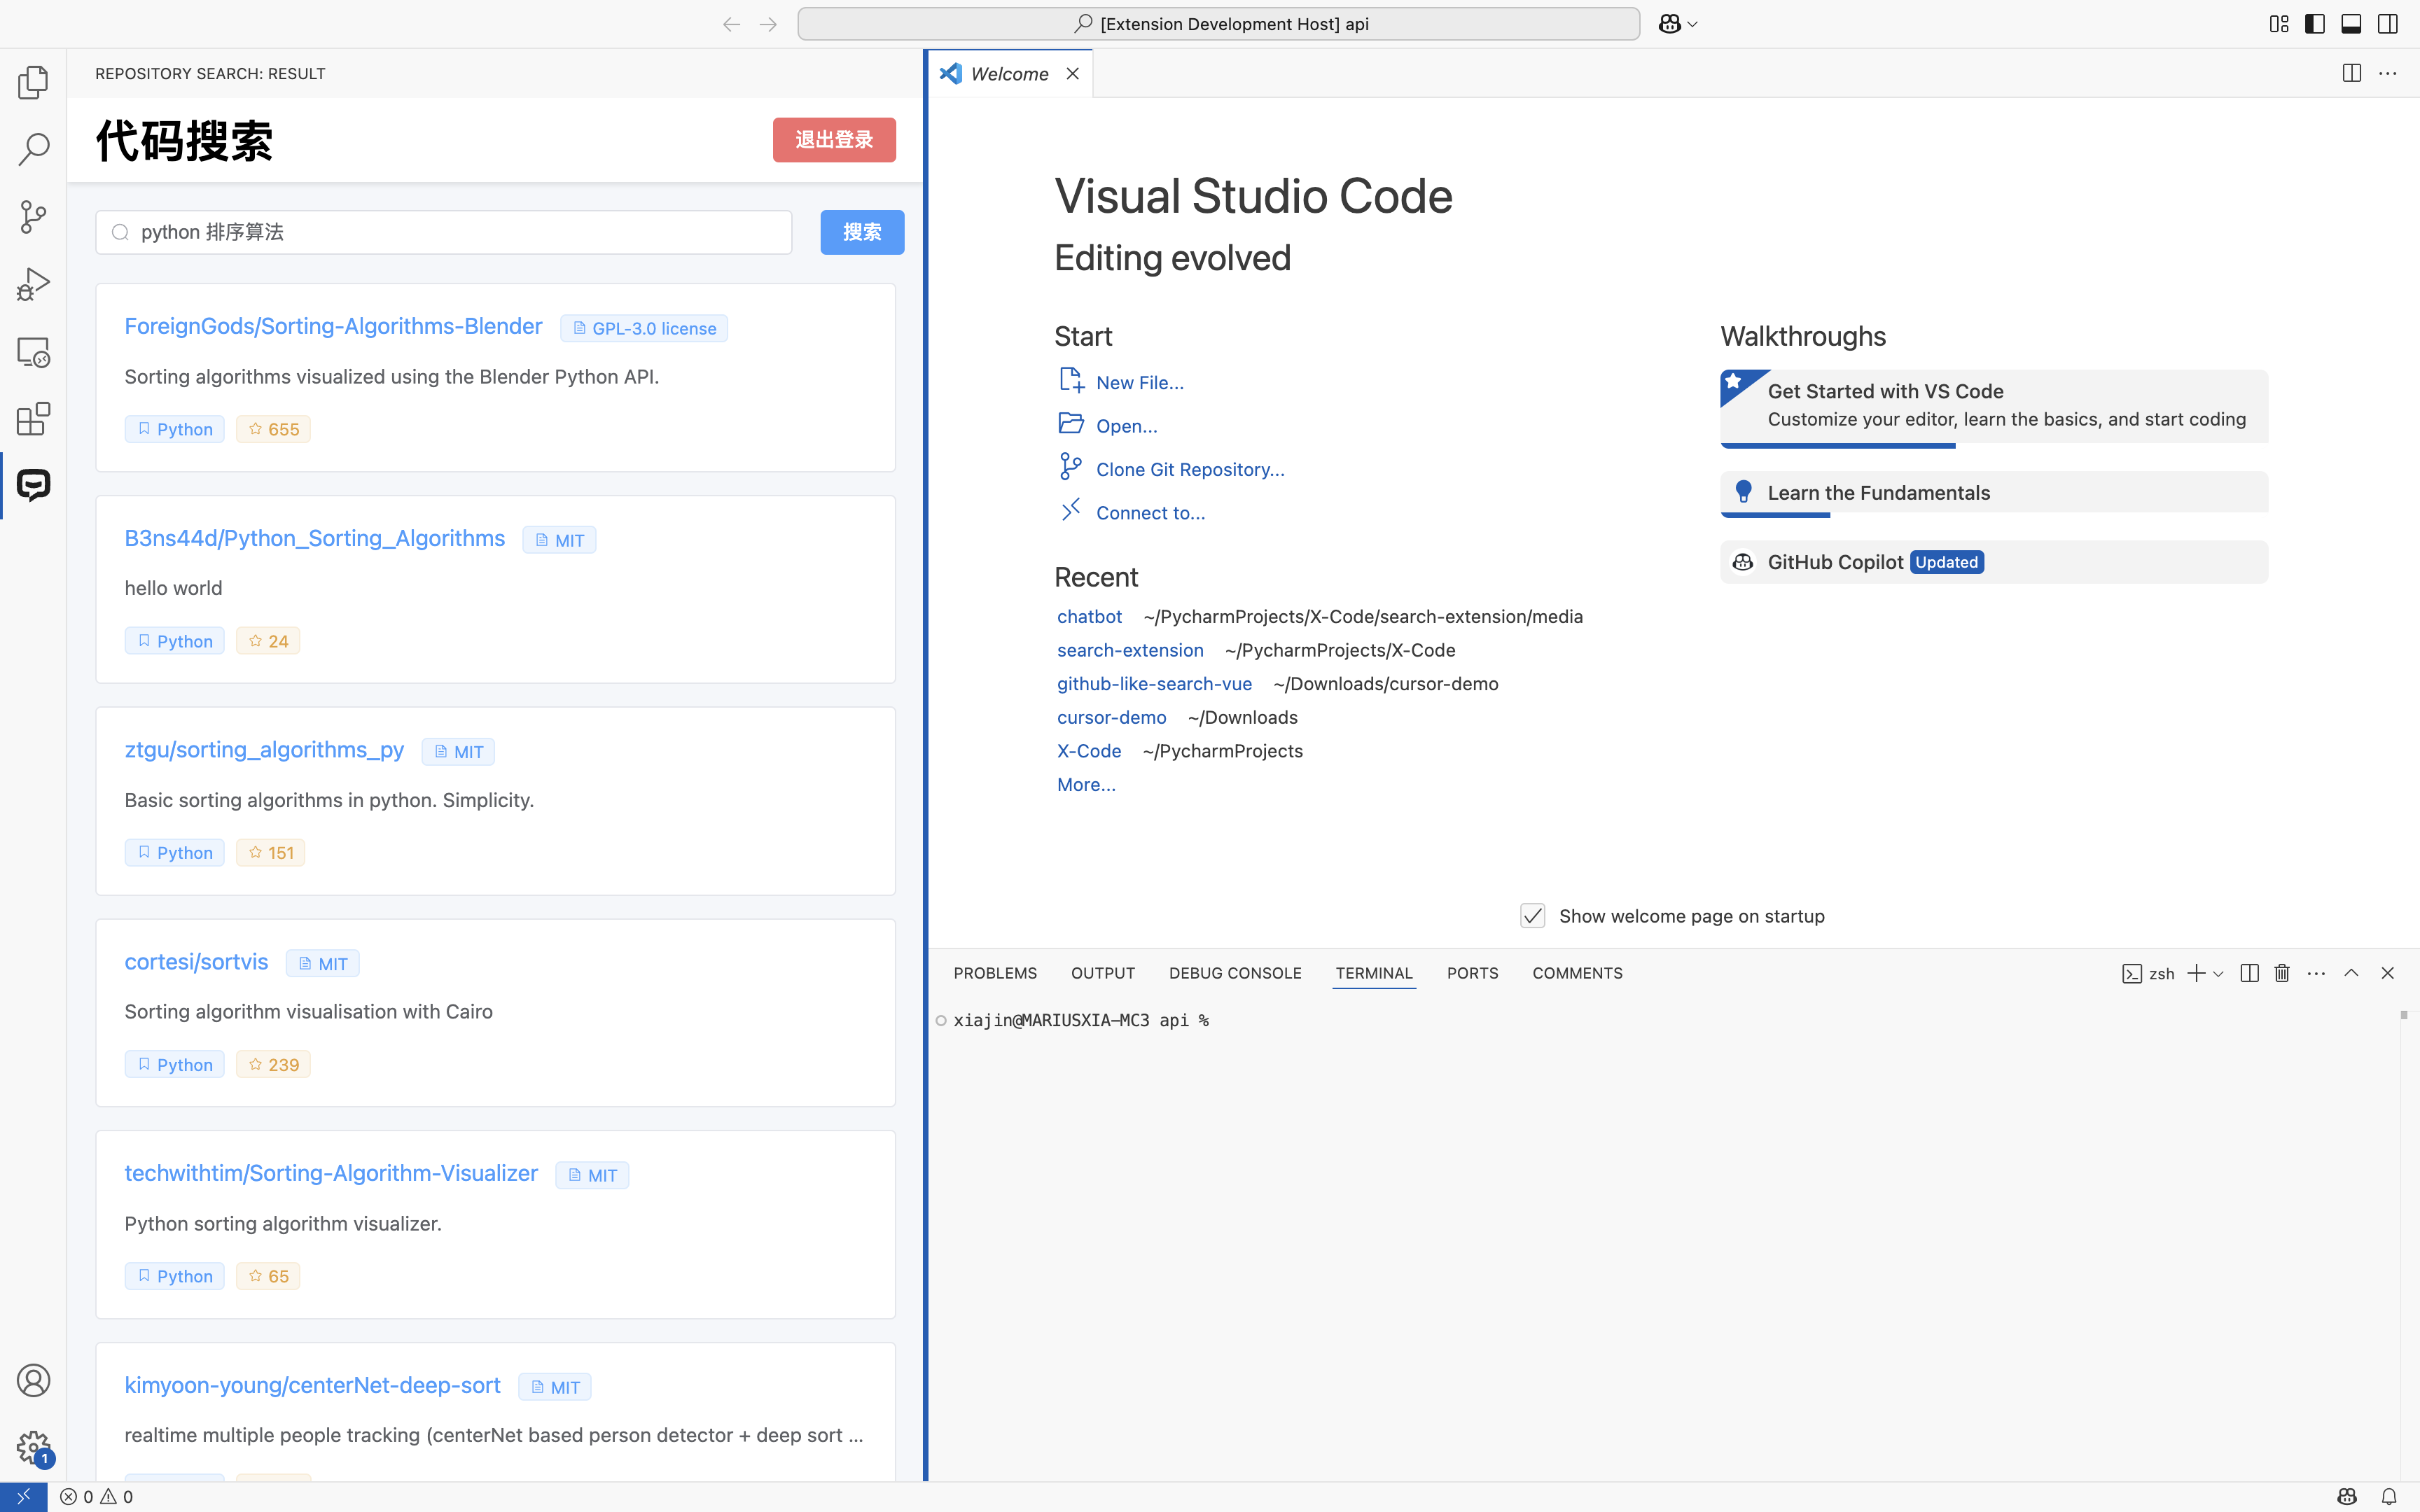
\includegraphics[width=0.95\textwidth]{search_page.png}}
	\caption{搜索页面示例}
	\label{searchpage}
\end{figure}
\begin{figure}[H]
	\center{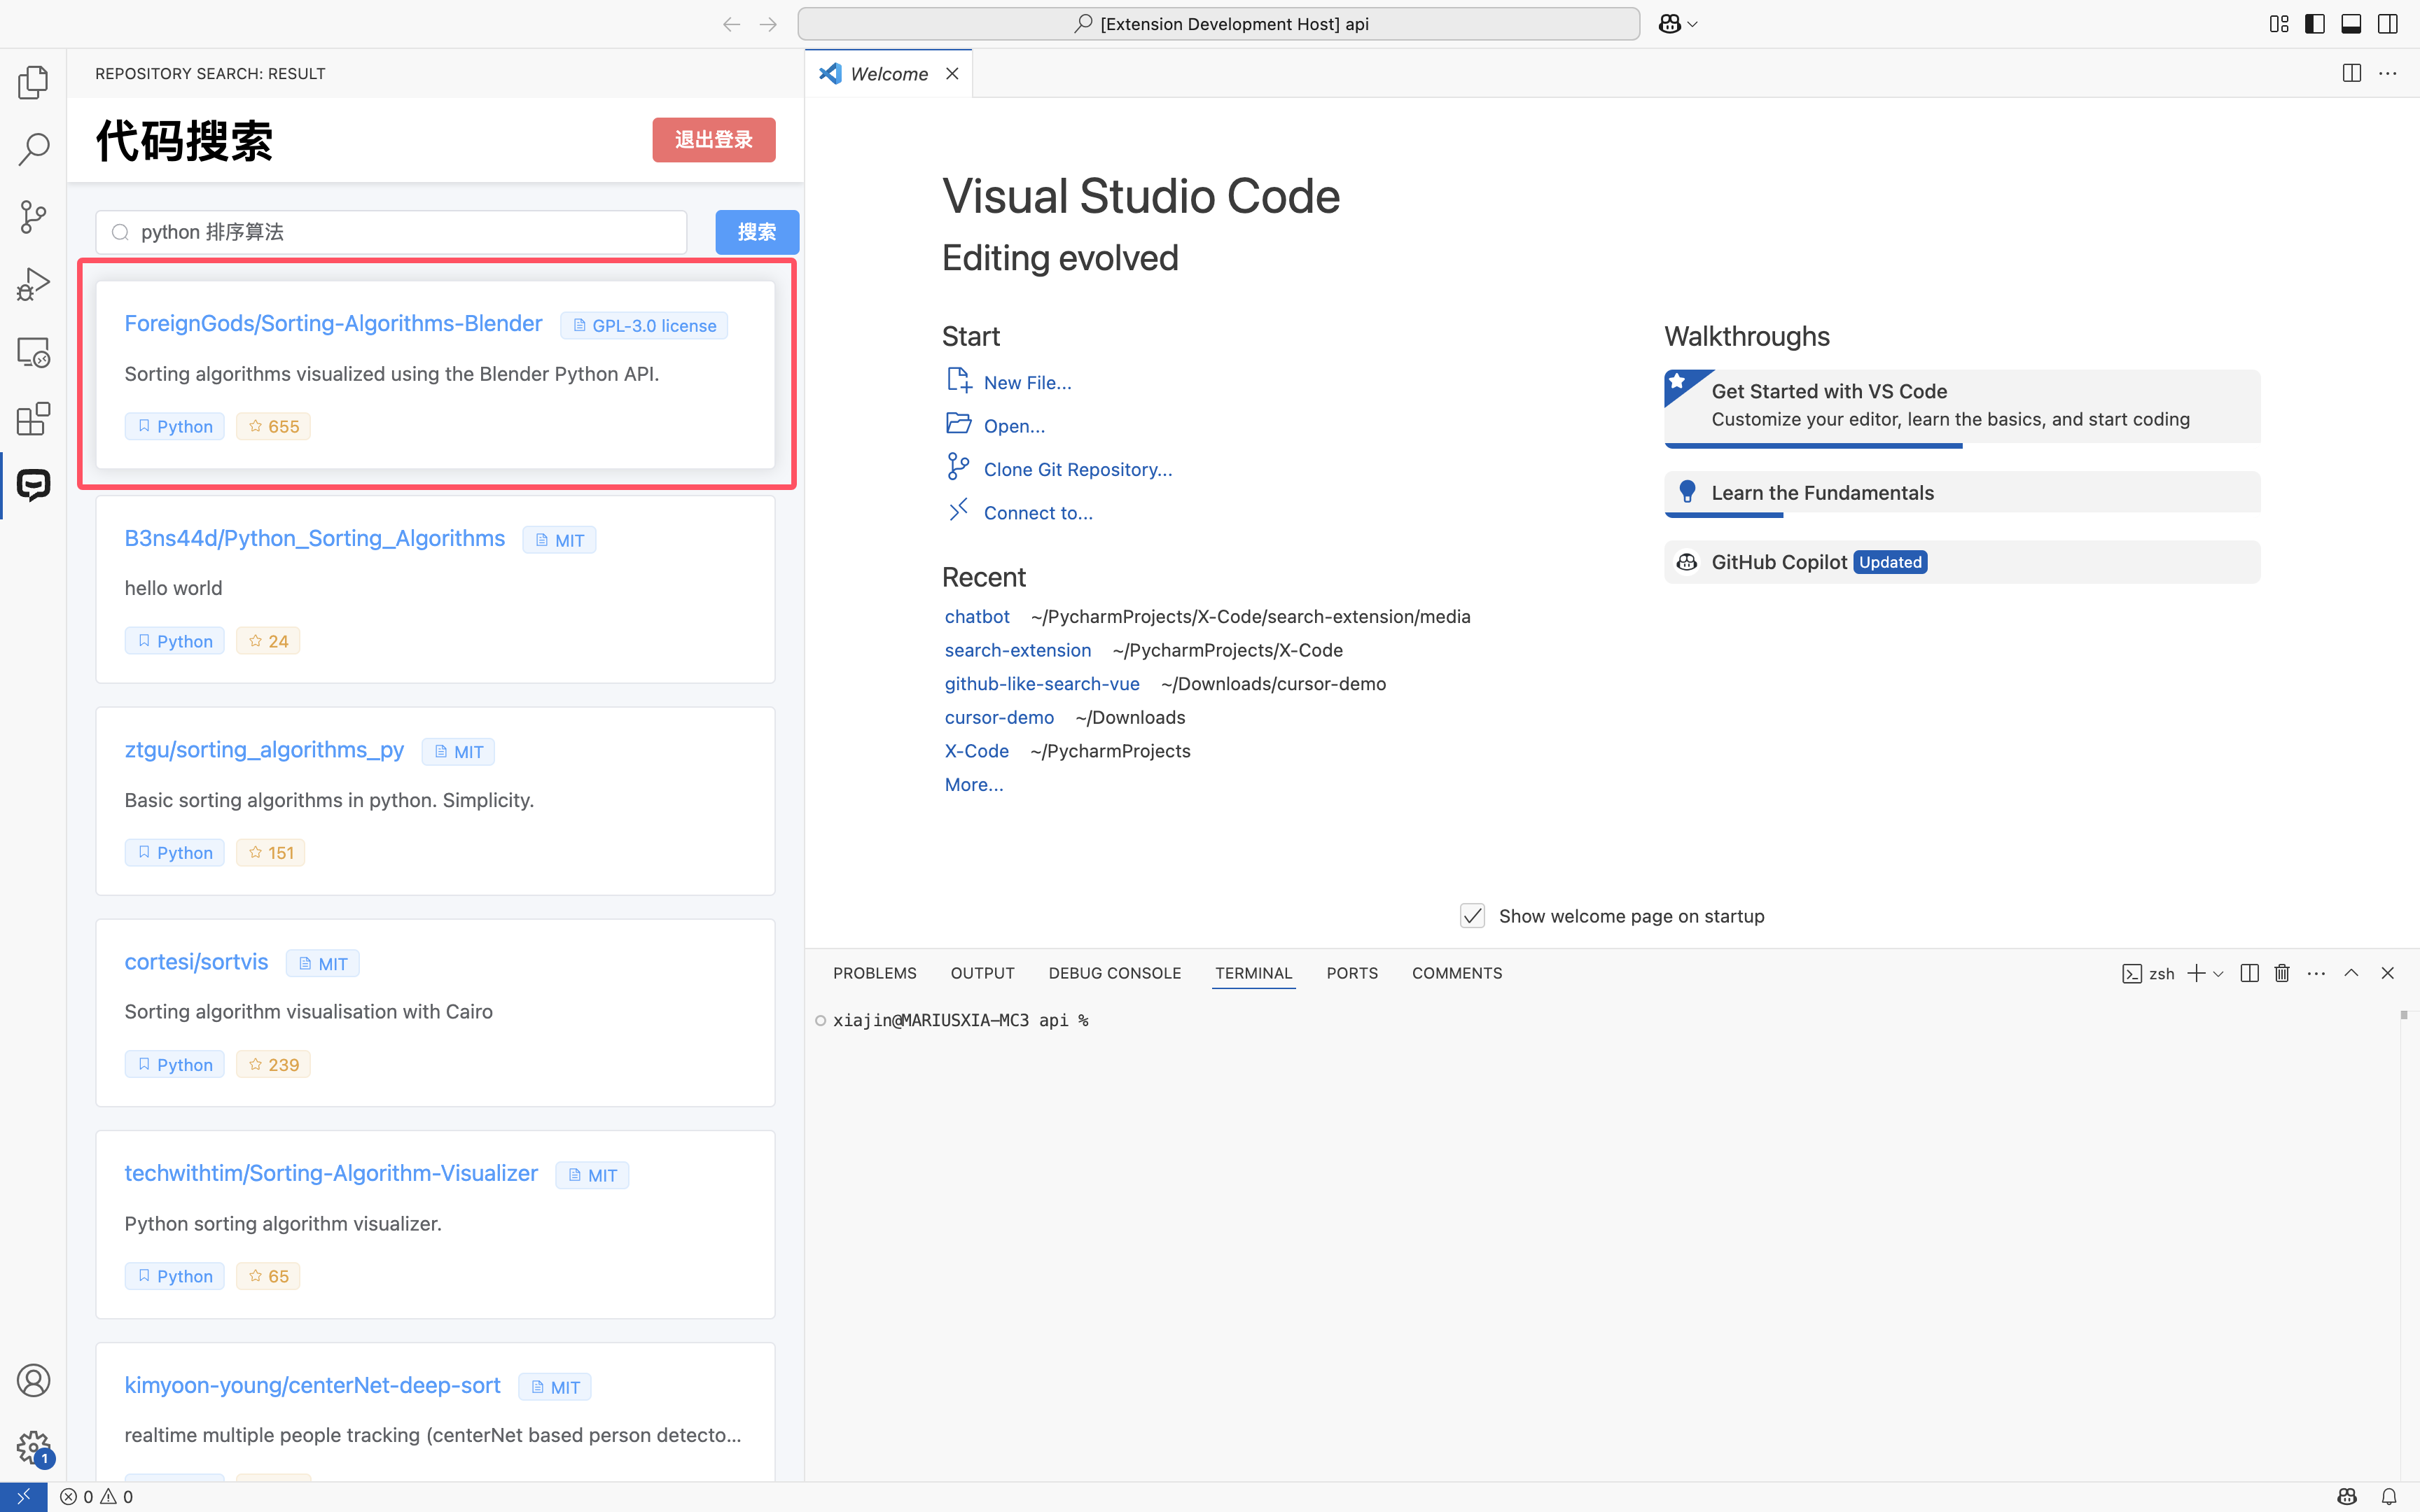
\includegraphics[width=0.95\textwidth]{search_select.png}}
	\caption{选中项目示例}
	\label{select}
\end{figure}
点击某一搜索结果后,用户可进入项目详情页面。该页面详细展示了项目名称、开源协议、项目描述、编程语言、星数、原始链接及文件列表,支持一键跳转至项目原网页,便于进一步浏览和分析。项目详情界面如图\ref{repodetailpage}所示。页面采用模块化布局,信息层次分明,支持文件树结构的动态展开与折叠,提升浏览效率。
\begin{figure}[H]
	\center{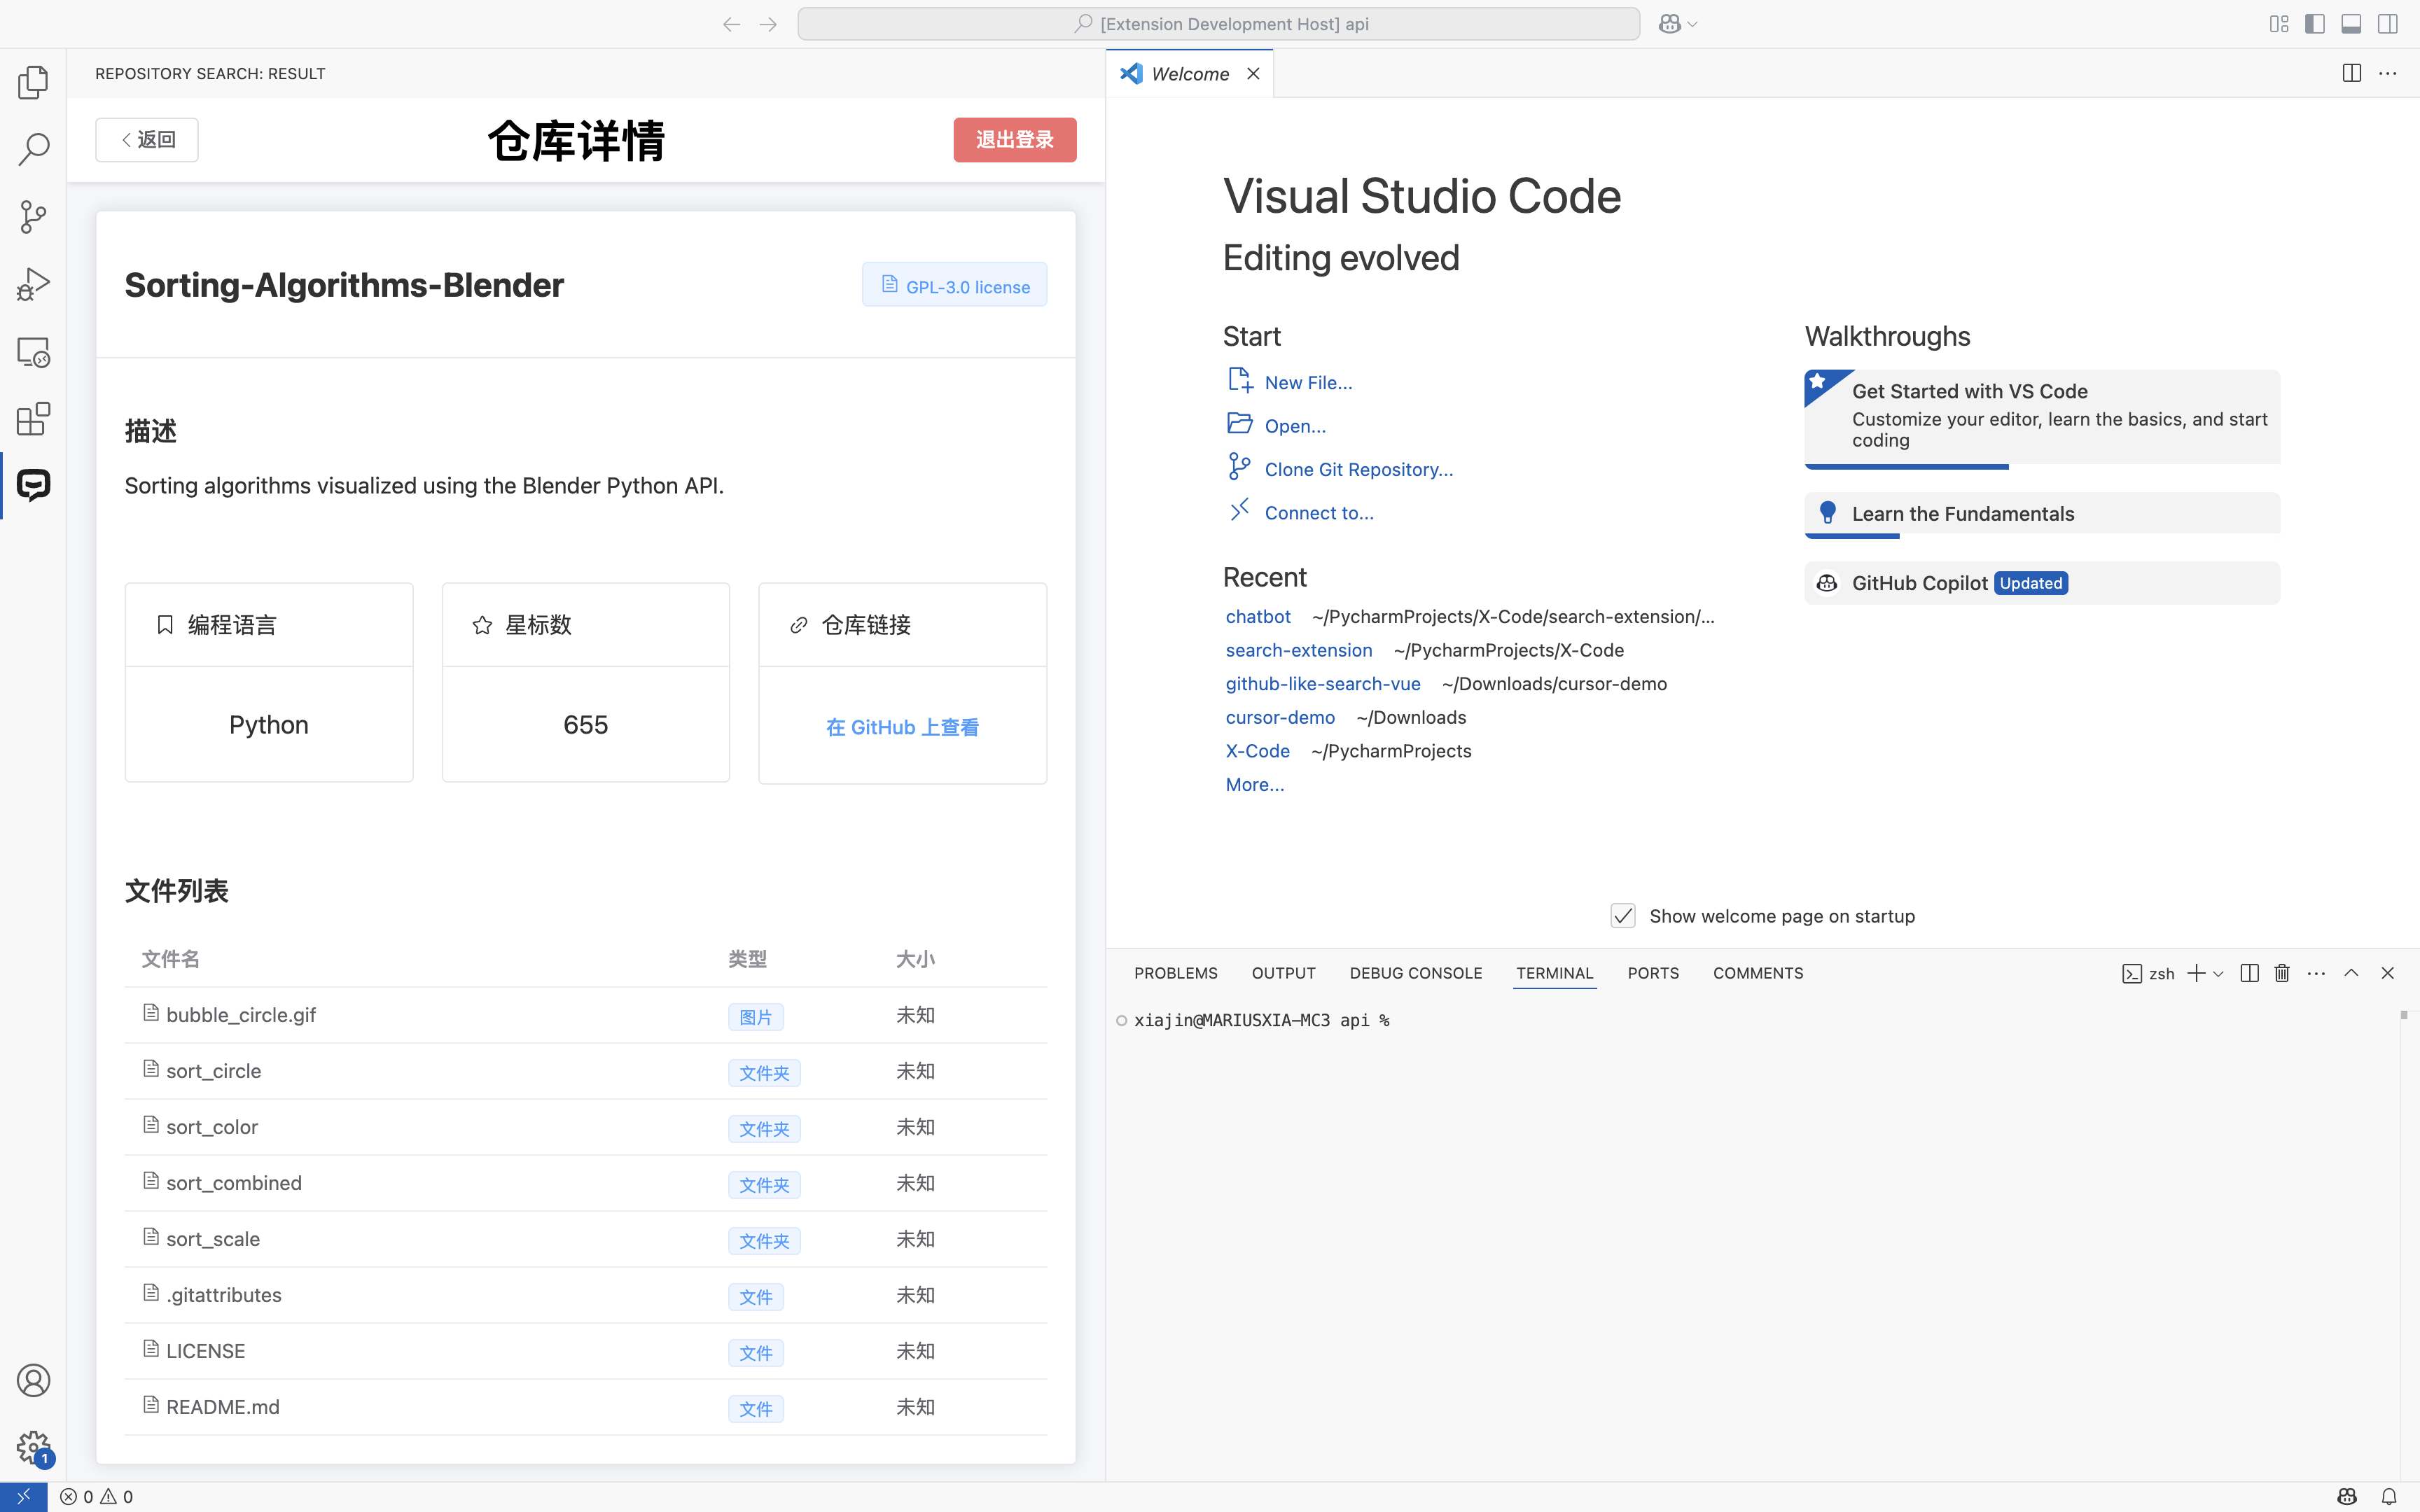
\includegraphics[width=0.95\textwidth]{repo_detail.png}}
	\caption{搜索详情示例}
	\label{repodetailpage}
\end{figure}
此外,前端系统通过Vuex实现全局状态管理,确保用户登录状态、搜索历史、检索结果等数据在各页面间同步更新。系统还集成了错误捕获与提示机制,针对网络异常、接口超时等情况给予友好反馈,保障用户操作的连续性和系统的稳定性。通过上述多端界面与分层架构的有机结合,系统实现了从用户注册、登录、代码检索到结果展示的完整闭环,极大提升了面向多编程语言的代码检索系统的易用性与用户体验。\par
\subsection{本章小结}
本章根据面向多编程语言的代码检索系统的设计方案,实现了从代码预处理、后端分布式架构、安全鉴权、到智能检索和前端界面设计的完整技术链条。基于AST的多语言代码结构化预处理模块,实现了对不同编程语言源代码的统一解析与规范化处理,为后续的语义分析和跨语言检索奠定了坚实基础。后端采用微服务架构,构建了高可用的统一接入网关、鉴权以及高性能可拓展的代码查询服务,保障了系统的安全性、稳定性及高并发处理能力。基于Elasticsearch的高性能分布式查询服务,实现了多维度、多语言的精准代码检索,结合大语言模型的查询意图理解与提示词工程,提升了检索的质量和结果相关性。在前端方面,系统通过Vue框架与VS Code插件的深度集成,提供了统一且友好的多端用户体验,支持注册登录的严格校验、智能搜索词预处理、结果高亮展示及项目详情的模块化浏览,确保用户操作的流畅性和系统的易用性。整体来看,本章实现方案充分体现了系统的模块化设计理念和技术先进性,为构建高效、智能且安全的多编程语言代码检索平台提供了坚实的技术实现。\par
\section{总结与展望}
本文围绕面向多编程语言的代码检索系统,系统性地提出并实现了一套高效、可扩展、智能化的技术方案。针对多语言代码的结构化难题,设计了基于AST的统一预处理流程,实现了不同编程语言代码的语法结构对齐和特征提取。系统采用前后端分离与微服务架构,结合高性能分布式查询引擎Elasticsearch和大语言模型,显著提升了检索的准确性、扩展性与系统的高可用性。在安全性方面,系统通过统一网关与鉴权服务,保障了用户数据和服务访问的安全。前端通过Vue框架与VS Code插件,为用户提供了便捷、直观的多端交互体验。通过提示词工程与上下文增强技术,系统进一步提升了对复杂检索意图的理解和响应能力。整体方案不仅满足了多编程语言环境下的高效代码检索需求,也为后续的智能化代码管理与开发辅助提供了坚实基础。\par
本项目在研发过程中,一种新的大语言模型协议正在重塑当前基于特定工作流的 AI Agent 结构。MCP 协议,基于大模型的 Function Call 能力,将外部工具能力以一种新的方式接入到大模型 Agent 中,正在重塑代码检索系统的交互范式与功能边界。未来,可将 MCP 协议深度融入系统架构,通过动态挂载代码分析工具、调试器、版本管理等外部组件,使检索系统具备 "智能执行" 能力 —— 用户发起检索请求时,系统不仅能返回代码片段,还可基于 MCP 协议调用工具链自动完成代码补全、错误诊断甚至自动化测试。此外,结合 MCP 协议的多轮对话机制,可构建更具逻辑性的检索引导流程,通过智能追问挖掘用户潜在需求,将传统的 "被动式检索" 升级为 "交互式代码创作助手"。\par

\newpage
\fancyhead[LH]{\zihao{-5}{\songti 重庆大学本科学生毕业论文(设计)}}
\fancyhead[RH]{\zihao{-5}{\songti 参考文献}}

\addcontentsline{toc}{section}{参考文献}
\renewcommand\refname{参考文献}

\zihao{5}

\begin{thebibliography}{1}
\setlength{\itemsep}{0pt}
\bibitem{ref1} Lv F, Zhang H, Lou J, et al. Codehow: Effective code search based on api understanding and extended boolean model (e)[C]//2015 30th IEEE/ACM International Conference on Automated Software Engineering (ASE). IEEE, 2015: 260-270.

\bibitem{ref2} Iyer S, Konstas I, Cheung A, et al. Summarizing source code using a neural attention model[C]//54th Annual Meeting of the Association for Computational Linguistics 2016. Association for Computational Linguistics, 2016: 2073-2083.

\bibitem{ref3} Han T, Xie W, Zisserman A. Self-supervised co-training for video representation learning[J]. Advances in neural information processing systems, 2020, 33: 5679-5690.

\bibitem{ref4} Qian S, Xu J, Liu Z, et al. UNIF: United neural implicit functions for clothed human reconstruction and animation[C]//European Conference on Computer Vision. Cham: Springer Nature Switzerland, 2022: 121-137.

\bibitem{ref5} Guo D, Ren S, Lu S, et al. Graphcodebert: Pre-training code representations with data flow[J]. arXiv preprint arXiv:2009.08366, 2020.

\bibitem{ref6} Husain H, Wu H H, Gazit T, et al. Codesearchnet challenge: Evaluating the state of semantic code search[J]. arXiv preprint arXiv:1909.09436, 2019.

\bibitem{ref7} Zhu M, Jain A, Suresh K, et al. Xlcost: A benchmark dataset for cross-lingual code intelligence[J]. arXiv preprint arXiv:2206.08474, 2022.

\bibitem{ref8} Mou L, Jin Z. Tree-based convolutional neural networks: principles and applications[M]. Singapore: Springer, 2018.

\bibitem{ref9} Feng Z, Guo D, Tang D, et al. Codebert: A pre-trained model for programming and natural languages[J]. arXiv preprint arXiv:2002.08155, 2020.

\bibitem{ref10} Ahmad W U, Chakraborty S, Ray B, et al. Unified pre-training for program understanding and generation[J]. arXiv preprint arXiv:2103.06333, 2021.

\bibitem{ref11} Guo D, Lu S, Duan N, et al. Unixcoder: Unified cross-modal pre-training for code representation[J]. arXiv preprint arXiv:2203.03850, 2022.

\bibitem{ref12} Shahi D. Apache Solr: an introduction[M]//Apache Solr: A practical approach to enterprise search. Berkeley, CA: Apress, 2015: 1-9.

\bibitem{ref13} Elasticsearch B V. Elasticsearch[J]. software], version, 2018, 6(1).

\bibitem{ref14} Vaswani A, Shazeer N, Parmar N, et al. Attention is all you need[J]. Advances in neural information processing systems, 2017, 30.

\bibitem{ref15} Jacobs R A, Jordan M I, Nowlan S J, et al. Adaptive mixtures of local experts[J]. Neural computation, 1991, 3(1): 79-87.

\bibitem{ref16}  Schulhoff S, Ilie M, Balepur N, et al. The prompt report: A systematic survey of prompting techniques[J]. arXiv preprint arXiv:2406.06608, 2024, 5.

\bibitem{ref17} Kojima T, Gu S S, Reid M, et al. Large language models are zero-shot reasoners[J]. Advances in neural information processing systems, 2022, 35: 22199-22213.
\bibitem{ref18} Reynolds L, McDonell K. Prompt programming for large language models: Beyond the few-shot paradigm[C]//Extended abstracts of the 2021 CHI conference on human factors in computing systems. 2021: 1-7.

\bibitem{ref19} Indrasiri K, Kuruppu D. gRPC: up and running: building cloud native applications with Go and Java for Docker and Kubernetes[M]. O'Reilly Media, 2020.

\bibitem{ref20} Docker I. Docker[J]. lınea].[Junio de 2017]. Disponible en: https://www. docker. com/what-docker, 2020.

\bibitem{ref21} Kubernetes T. Kubernetes[J]. Kubernetes. Retrieved May, 2019, 24: 2019.


\end{thebibliography}
%(参考文献格式请参考GB/T 7714-2015《信息与文献 参考文献著录规则》)

\newpage
\fancyhead[LH]{\zihao{-5}{\songti 重庆大学本科学生毕业论文(设计)}}
\fancyhead[RH]{\zihao{-5}{\songti 致谢}}

\addcontentsline{toc}{section}{致谢}
\renewcommand\refname{致谢}

\section*{致\quad 谢}
\zihao{-4}
致谢主要感谢导师和对论文工作有直接贡献和帮助的人士和单位。致谢言语应谦虚诚恳,实事求是。

\newpage
\thispagestyle{empty}

\addcontentsline{toc}{section}{原创性声明和使用授权书}
\begin{center}
\heiti \zihao{3}
原创性声明
\end{center}

\songti\zihao{-4}
郑重声明:所呈交的论文(设计)\underline{《  \hspace{6em}》},是本人在导师的指导下,独立进行研究取得的成果。除论文(设计)中已经标注引用的内容外,本论文(设计)不包含其他人或集体已经发表或撰写过的作品成果。对本文的研究做出贡献的个人和集体,均已在文中以明确方式标明。本人完全意识到本声明的法律后果,并承诺因本声明而产生的法律结果由本人承担。

~\\
\begin{flushleft}
\begin{tabular}{l}
\songti\zihao{-4}
论文(设计)作者签名: \underline{\hspace{6em}}\\
\songti\zihao{-4}
日期:\underline{\hspace{6em}}
\end{tabular}
\end{flushleft}

~\\
\begin{center}
\heiti \zihao{3}
使用授权书
\end{center}

\songti\zihao{-4}
本论文(设计)作者完全了解学校有关保留、使用论文(设计)的规定,同意学校保留并向国家有关部门或机构送交论文(设计)复印件和电子版,允许论文(设计)被查阅和借阅。本人授权重庆大学将本论文(设计)的全部或部分内容编入有关数据库进行检索,可以采用影印、缩印或扫描等复制方式保存和汇编本论文(设计)。

~\\
\songti\zihao{-4}
本论文(设计)属于:\par
保\quad 密 $\Box$  \quad 在\underline{\qquad}年解密后适用本授权书\par
不保密 $\Box$

~\\
~\\
\begin{flushleft}
\songti\zihao{-4}
\begin{tabular}{l l}
论文(设计)作者签名:\underline{\hspace{6em}} \hspace{300mm}&指导教师签名:\underline{\hspace{6em}} \\
日期:\underline{\hspace{6em}} &日期:\underline{\hspace{6em}}\\
\end{tabular}
\end{flushleft}

\end{document} 